\documentclass{book}
\usepackage[a4paper,top=2.5cm,bottom=2.5cm,left=2.5cm,right=2.5cm]{geometry}
\usepackage{makeidx}
\usepackage{natbib}
\usepackage{graphicx}
\usepackage{multicol}
\usepackage{float}
\usepackage{listings}
\usepackage{color}
\usepackage{ifthen}
\usepackage[table]{xcolor}
\usepackage{textcomp}
\usepackage{alltt}
\usepackage{ifpdf}
\ifpdf
\usepackage[pdftex,
            pagebackref=true,
            colorlinks=true,
            linkcolor=blue,
            unicode
           ]{hyperref}
\else
\usepackage[ps2pdf,
            pagebackref=true,
            colorlinks=true,
            linkcolor=blue,
            unicode
           ]{hyperref}
\usepackage{pspicture}
\fi
\usepackage[utf8]{inputenc}
\usepackage{mathptmx}
\usepackage[scaled=.90]{helvet}
\usepackage{courier}
\usepackage{sectsty}
\usepackage{amssymb}
\usepackage[titles]{tocloft}
\usepackage{doxygen}
\lstset{language=C++,inputencoding=utf8,basicstyle=\footnotesize,breaklines=true,breakatwhitespace=true,tabsize=4,numbers=left }
\makeindex
\setcounter{tocdepth}{3}
\renewcommand{\footrulewidth}{0.4pt}
\renewcommand{\familydefault}{\sfdefault}
\hfuzz=15pt
\setlength{\emergencystretch}{15pt}
\hbadness=750
\tolerance=750
\begin{document}
\hypersetup{pageanchor=false,citecolor=blue}
\begin{titlepage}
\vspace*{7cm}
\begin{center}
{\Large Reference Manual}\\
\vspace*{1cm}
{\large Generated by Doxygen 1.8.3.1}\\
\vspace*{0.5cm}
{\small Mon Mar 10 2014 08:37:30}\\
\end{center}
\end{titlepage}
\clearemptydoublepage
\pagenumbering{roman}
\tableofcontents
\clearemptydoublepage
\pagenumbering{arabic}
\hypersetup{pageanchor=true,citecolor=blue}
\chapter{Module Index}
\section{Modules}
Here is a list of all modules\-:\begin{DoxyCompactList}
\item \contentsline{section}{R\-T\-O\-S}{\pageref{group___r_t_o_s}}{}
\end{DoxyCompactList}

\chapter{Hierarchical Index}
\section{Class Hierarchy}
This inheritance list is sorted roughly, but not completely, alphabetically\-:\begin{DoxyCompactList}
\item \contentsline{section}{eeprom}{\pageref{structeeprom}}{}
\item Frame\begin{DoxyCompactList}
\item \contentsline{section}{Main\-Window}{\pageref{classarbitros_ahrs_1_1_main_window}}{}
\end{DoxyCompactList}
\item G\-L\-Canvas\begin{DoxyCompactList}
\item \contentsline{section}{My\-Canvas\-Base}{\pageref{classarbitros_ahrs_1_1_my_canvas_base}}{}
\begin{DoxyCompactList}
\item \contentsline{section}{Cube\-Canvas}{\pageref{classarbitros_ahrs_1_1_cube_canvas}}{}
\item \contentsline{section}{Xy\-Plot\-Accel}{\pageref{classarbitros_ahrs_1_1_xy_plot_accel}}{}
\item \contentsline{section}{Xy\-Plot\-Gyro}{\pageref{classarbitros_ahrs_1_1_xy_plot_gyro}}{}
\item \contentsline{section}{Xy\-Plot\-Mag}{\pageref{classarbitros_ahrs_1_1_xy_plot_mag}}{}
\end{DoxyCompactList}
\end{DoxyCompactList}
\item \contentsline{section}{list\-Link}{\pageref{structlist_link}}{}
\item \contentsline{section}{t\-\_\-accel\-Dev}{\pageref{structt__accel_dev}}{}
\item \contentsline{section}{t\-\_\-adc\-Chan\-Conf}{\pageref{structt__adc_chan_conf}}{}
\item \contentsline{section}{t\-\_\-adc\-Mod\-Conf}{\pageref{structt__adc_mod_conf}}{}
\item \contentsline{section}{t\-\_\-arb\-Comm\-Dev}{\pageref{structt__arb_comm_dev}}{}
\item \contentsline{section}{t\-\_\-arb\-Comm\-Setup}{\pageref{structt__arb_comm_setup}}{}
\item \contentsline{section}{t\-\_\-buffer\-Handle}{\pageref{structt__buffer_handle}}{}
\item \contentsline{section}{t\-\_\-card\-Info\-Msg}{\pageref{structt__card_info_msg}}{}
\item \contentsline{section}{t\-\_\-chan\-Handle}{\pageref{structt__chan_handle}}{}
\item \contentsline{section}{t\-\_\-clocks}{\pageref{structt__clocks}}{}
\item \contentsline{section}{t\-\_\-console\-Dev}{\pageref{structt__console_dev}}{}
\item \contentsline{section}{t\-\_\-console\-Object}{\pageref{structt__console_object}}{}
\item \contentsline{section}{t\-\_\-console\-Setup}{\pageref{structt__console_setup}}{}
\item \contentsline{section}{t\-\_\-console\-Tok\-Hndl}{\pageref{structt__console_tok_hndl}}{}
\item \contentsline{section}{t\-\_\-curs\-Pos}{\pageref{structt__curs_pos}}{}
\item \contentsline{section}{t\-\_\-cust\-Char}{\pageref{structt__cust_char}}{}
\item \contentsline{section}{t\-\_\-dev\-Handle}{\pageref{structt__dev_handle}}{}
\item \contentsline{section}{t\-\_\-device}{\pageref{structt__device}}{}
\item \contentsline{section}{t\-\_\-device\-Operations}{\pageref{structt__device_operations}}{}
\item \contentsline{section}{t\-\_\-dma\-Chan}{\pageref{structt__dma_chan}}{}
\item \contentsline{section}{t\-\_\-dma\-Chan\-Config}{\pageref{structt__dma_chan_config}}{}
\item \contentsline{section}{t\-\_\-dma\-Cntrl\-Config}{\pageref{structt__dma_cntrl_config}}{}
\item \contentsline{section}{t\-\_\-dma\-Int\-Hndl}{\pageref{structt__dma_int_hndl}}{}
\item \contentsline{section}{t\-\_\-eeprom\-List}{\pageref{structt__eeprom_list}}{}
\item \contentsline{section}{t\-\_\-ellipsoid\-Cal}{\pageref{structt__ellipsoid_cal}}{}
\item \contentsline{section}{t\-\_\-gpio\-Conf}{\pageref{structt__gpio_conf}}{}
\item \contentsline{section}{t\-\_\-gpio\-Int\-Hndl}{\pageref{structt__gpio_int_hndl}}{}
\item \contentsline{section}{t\-\_\-gyro\-Dev}{\pageref{structt__gyro_dev}}{}
\item \contentsline{section}{t\-\_\-idle\-Object}{\pageref{structt__idle_object}}{}
\item \contentsline{section}{t\-\_\-ins\-Dev}{\pageref{structt__ins_dev}}{}
\item \contentsline{section}{t\-\_\-int\-Chan\-Map}{\pageref{structt__int_chan_map}}{}
\item \contentsline{section}{t\-\_\-int\-Conf}{\pageref{structt__int_conf}}{}
\item \contentsline{section}{t\-\_\-lcd\-Dev}{\pageref{structt__lcd_dev}}{}
\item \contentsline{section}{t\-\_\-lcd\-Setup}{\pageref{structt__lcd_setup}}{}
\item \contentsline{section}{t\-\_\-list\-Container}{\pageref{structt__list_container}}{}
\item \contentsline{section}{t\-\_\-mag\-Dev}{\pageref{structt__mag_dev}}{}
\item \contentsline{section}{t\-\_\-mailbox}{\pageref{structt__mailbox}}{}
\item \contentsline{section}{t\-\_\-mailbox\-Config}{\pageref{structt__mailbox_config}}{}
\item \contentsline{section}{t\-\_\-math\-Objct}{\pageref{structt__math_objct}}{}
\item \contentsline{section}{t\-\_\-nav\-Struct}{\pageref{structt__nav_struct}}{}
\item \contentsline{section}{t\-\_\-pan\-Tilt\-Dev}{\pageref{structt__pan_tilt_dev}}{}
\item \contentsline{section}{t\-\_\-platform\-Test\-Object}{\pageref{structt__platform_test_object}}{}
\item \contentsline{section}{t\-\_\-print\-Object}{\pageref{structt__print_object}}{}
\item \contentsline{section}{t\-\_\-pwr\-Object}{\pageref{structt__pwr_object}}{}
\item \contentsline{section}{t\-\_\-sched\-Object}{\pageref{structt__sched_object}}{}
\item \contentsline{section}{t\-\_\-sd\-Dev}{\pageref{structt__sd_dev}}{}
\item \contentsline{section}{t\-\_\-sd\-Setup}{\pageref{structt__sd_setup}}{}
\item \contentsline{section}{t\-\_\-sem}{\pageref{structt__sem}}{}
\item \contentsline{section}{t\-\_\-signal\-Dev}{\pageref{structt__signal_dev}}{}
\item \contentsline{section}{t\-\_\-signal\-Setup}{\pageref{structt__signal_setup}}{}
\item \contentsline{section}{t\-\_\-sonar\-Dev}{\pageref{structt__sonar_dev}}{}
\item \contentsline{section}{t\-\_\-spi\-Chan\-Hndl}{\pageref{structt__spi_chan_hndl}}{}
\item \contentsline{section}{t\-\_\-spi\-Config}{\pageref{structt__spi_config}}{}
\item \contentsline{section}{t\-\_\-spi\-User\-Hndl}{\pageref{structt__spi_user_hndl}}{}
\item \contentsline{section}{t\-\_\-st\-Mn\-Object}{\pageref{structt__st_mn_object}}{}
\item \contentsline{section}{t\-\_\-sys\-Time}{\pageref{structt__sys_time}}{}
\item \contentsline{section}{t\-\_\-template\-Dev}{\pageref{structt__template_dev}}{}
\item \contentsline{section}{t\-\_\-timer\-Config}{\pageref{structt__timer_config}}{}
\item \contentsline{section}{t\-\_\-twi\-Config}{\pageref{structt__twi_config}}{}
\item \contentsline{section}{t\-\_\-type\-Punn}{\pageref{uniont__type_punn}}{}
\item \contentsline{section}{t\-\_\-uart\-Chan\-Hndl}{\pageref{structt__uart_chan_hndl}}{}
\item \contentsline{section}{t\-\_\-uart\-Config}{\pageref{structt__uart_config}}{}
\item \contentsline{section}{t\-\_\-wd\-Config}{\pageref{structt__wd_config}}{}
\item \contentsline{section}{t\-\_\-wd\-Object}{\pageref{structt__wd_object}}{}
\item \contentsline{section}{t\-\_\-wifly\-Config}{\pageref{structt__wifly_config}}{}
\item \contentsline{section}{t\-\_\-wifly\-Dev}{\pageref{structt__wifly_dev}}{}
\item \contentsline{section}{t\-\_\-wifly\-Setup}{\pageref{structt__wifly_setup}}{}
\item \contentsline{section}{T\-C\-B}{\pageref{struct_t_c_b}}{}
\item \contentsline{section}{timer\-Int}{\pageref{structtimer_int}}{}
\item \contentsline{section}{timer\-Mod}{\pageref{structtimer_mod}}{}
\item \contentsline{section}{twi\-Chan\-Hndl}{\pageref{structtwi_chan_hndl}}{}
\end{DoxyCompactList}

\chapter{Data Structure Index}
\section{Data Structures}
Here are the data structures with brief descriptions\-:\begin{DoxyCompactList}
\item\contentsline{section}{\hyperlink{classarbitros_ahrs_1_1_cube_canvas}{Cube\-Canvas} }{\pageref{classarbitros_ahrs_1_1_cube_canvas}}{}
\item\contentsline{section}{\hyperlink{structeeprom}{eeprom} }{\pageref{structeeprom}}{}
\item\contentsline{section}{\hyperlink{structlist_link}{list\-Link} }{\pageref{structlist_link}}{}
\item\contentsline{section}{\hyperlink{classarbitros_ahrs_1_1_main_window}{Main\-Window} }{\pageref{classarbitros_ahrs_1_1_main_window}}{}
\item\contentsline{section}{\hyperlink{classarbitros_ahrs_1_1_my_canvas_base}{My\-Canvas\-Base} }{\pageref{classarbitros_ahrs_1_1_my_canvas_base}}{}
\item\contentsline{section}{\hyperlink{structt__accel_dev}{t\-\_\-accel\-Dev} }{\pageref{structt__accel_dev}}{}
\item\contentsline{section}{\hyperlink{structt__adc_chan_conf}{t\-\_\-adc\-Chan\-Conf} }{\pageref{structt__adc_chan_conf}}{}
\item\contentsline{section}{\hyperlink{structt__adc_mod_conf}{t\-\_\-adc\-Mod\-Conf} }{\pageref{structt__adc_mod_conf}}{}
\item\contentsline{section}{\hyperlink{structt__arb_comm_dev}{t\-\_\-arb\-Comm\-Dev} }{\pageref{structt__arb_comm_dev}}{}
\item\contentsline{section}{\hyperlink{structt__arb_comm_setup}{t\-\_\-arb\-Comm\-Setup} }{\pageref{structt__arb_comm_setup}}{}
\item\contentsline{section}{\hyperlink{structt__buffer_handle}{t\-\_\-buffer\-Handle} }{\pageref{structt__buffer_handle}}{}
\item\contentsline{section}{\hyperlink{structt__card_info_msg}{t\-\_\-card\-Info\-Msg} }{\pageref{structt__card_info_msg}}{}
\item\contentsline{section}{\hyperlink{structt__chan_handle}{t\-\_\-chan\-Handle} }{\pageref{structt__chan_handle}}{}
\item\contentsline{section}{\hyperlink{structt__clocks}{t\-\_\-clocks} }{\pageref{structt__clocks}}{}
\item\contentsline{section}{\hyperlink{structt__console_dev}{t\-\_\-console\-Dev} }{\pageref{structt__console_dev}}{}
\item\contentsline{section}{\hyperlink{structt__console_object}{t\-\_\-console\-Object} \\*Grouping of objects commonly used across all functions within this file }{\pageref{structt__console_object}}{}
\item\contentsline{section}{\hyperlink{structt__console_setup}{t\-\_\-console\-Setup} }{\pageref{structt__console_setup}}{}
\item\contentsline{section}{\hyperlink{structt__console_tok_hndl}{t\-\_\-console\-Tok\-Hndl} }{\pageref{structt__console_tok_hndl}}{}
\item\contentsline{section}{\hyperlink{structt__curs_pos}{t\-\_\-curs\-Pos} }{\pageref{structt__curs_pos}}{}
\item\contentsline{section}{\hyperlink{structt__cust_char}{t\-\_\-cust\-Char} }{\pageref{structt__cust_char}}{}
\item\contentsline{section}{\hyperlink{structt__dev_handle}{t\-\_\-dev\-Handle} }{\pageref{structt__dev_handle}}{}
\item\contentsline{section}{\hyperlink{structt__device}{t\-\_\-device} }{\pageref{structt__device}}{}
\item\contentsline{section}{\hyperlink{structt__device_operations}{t\-\_\-device\-Operations} }{\pageref{structt__device_operations}}{}
\item\contentsline{section}{\hyperlink{structt__dma_chan}{t\-\_\-dma\-Chan} }{\pageref{structt__dma_chan}}{}
\item\contentsline{section}{\hyperlink{structt__dma_chan_config}{t\-\_\-dma\-Chan\-Config} }{\pageref{structt__dma_chan_config}}{}
\item\contentsline{section}{\hyperlink{structt__dma_cntrl_config}{t\-\_\-dma\-Cntrl\-Config} }{\pageref{structt__dma_cntrl_config}}{}
\item\contentsline{section}{\hyperlink{structt__dma_int_hndl}{t\-\_\-dma\-Int\-Hndl} }{\pageref{structt__dma_int_hndl}}{}
\item\contentsline{section}{\hyperlink{structt__eeprom_list}{t\-\_\-eeprom\-List} }{\pageref{structt__eeprom_list}}{}
\item\contentsline{section}{\hyperlink{structt__ellipsoid_cal}{t\-\_\-ellipsoid\-Cal} }{\pageref{structt__ellipsoid_cal}}{}
\item\contentsline{section}{\hyperlink{structt__gpio_conf}{t\-\_\-gpio\-Conf} }{\pageref{structt__gpio_conf}}{}
\item\contentsline{section}{\hyperlink{structt__gpio_int_hndl}{t\-\_\-gpio\-Int\-Hndl} }{\pageref{structt__gpio_int_hndl}}{}
\item\contentsline{section}{\hyperlink{structt__gyro_dev}{t\-\_\-gyro\-Dev} }{\pageref{structt__gyro_dev}}{}
\item\contentsline{section}{\hyperlink{structt__idle_object}{t\-\_\-idle\-Object} }{\pageref{structt__idle_object}}{}
\item\contentsline{section}{\hyperlink{structt__ins_dev}{t\-\_\-ins\-Dev} }{\pageref{structt__ins_dev}}{}
\item\contentsline{section}{\hyperlink{structt__int_chan_map}{t\-\_\-int\-Chan\-Map} }{\pageref{structt__int_chan_map}}{}
\item\contentsline{section}{\hyperlink{structt__int_conf}{t\-\_\-int\-Conf} }{\pageref{structt__int_conf}}{}
\item\contentsline{section}{\hyperlink{structt__lcd_dev}{t\-\_\-lcd\-Dev} }{\pageref{structt__lcd_dev}}{}
\item\contentsline{section}{\hyperlink{structt__lcd_setup}{t\-\_\-lcd\-Setup} }{\pageref{structt__lcd_setup}}{}
\item\contentsline{section}{\hyperlink{structt__list_container}{t\-\_\-list\-Container} }{\pageref{structt__list_container}}{}
\item\contentsline{section}{\hyperlink{structt__mag_dev}{t\-\_\-mag\-Dev} }{\pageref{structt__mag_dev}}{}
\item\contentsline{section}{\hyperlink{structt__mailbox}{t\-\_\-mailbox} }{\pageref{structt__mailbox}}{}
\item\contentsline{section}{\hyperlink{structt__mailbox_config}{t\-\_\-mailbox\-Config} }{\pageref{structt__mailbox_config}}{}
\item\contentsline{section}{\hyperlink{structt__math_objct}{t\-\_\-math\-Objct} }{\pageref{structt__math_objct}}{}
\item\contentsline{section}{\hyperlink{structt__nav_struct}{t\-\_\-nav\-Struct} }{\pageref{structt__nav_struct}}{}
\item\contentsline{section}{\hyperlink{structt__pan_tilt_dev}{t\-\_\-pan\-Tilt\-Dev} }{\pageref{structt__pan_tilt_dev}}{}
\item\contentsline{section}{\hyperlink{structt__platform_test_object}{t\-\_\-platform\-Test\-Object} }{\pageref{structt__platform_test_object}}{}
\item\contentsline{section}{\hyperlink{structt__print_object}{t\-\_\-print\-Object} }{\pageref{structt__print_object}}{}
\item\contentsline{section}{\hyperlink{structt__pwr_object}{t\-\_\-pwr\-Object} }{\pageref{structt__pwr_object}}{}
\item\contentsline{section}{\hyperlink{structt__sched_object}{t\-\_\-sched\-Object} }{\pageref{structt__sched_object}}{}
\item\contentsline{section}{\hyperlink{structt__sd_dev}{t\-\_\-sd\-Dev} }{\pageref{structt__sd_dev}}{}
\item\contentsline{section}{\hyperlink{structt__sd_setup}{t\-\_\-sd\-Setup} }{\pageref{structt__sd_setup}}{}
\item\contentsline{section}{\hyperlink{structt__sem}{t\-\_\-sem} }{\pageref{structt__sem}}{}
\item\contentsline{section}{\hyperlink{structt__signal_dev}{t\-\_\-signal\-Dev} }{\pageref{structt__signal_dev}}{}
\item\contentsline{section}{\hyperlink{structt__signal_setup}{t\-\_\-signal\-Setup} }{\pageref{structt__signal_setup}}{}
\item\contentsline{section}{\hyperlink{structt__sonar_dev}{t\-\_\-sonar\-Dev} }{\pageref{structt__sonar_dev}}{}
\item\contentsline{section}{\hyperlink{structt__spi_chan_hndl}{t\-\_\-spi\-Chan\-Hndl} }{\pageref{structt__spi_chan_hndl}}{}
\item\contentsline{section}{\hyperlink{structt__spi_config}{t\-\_\-spi\-Config} }{\pageref{structt__spi_config}}{}
\item\contentsline{section}{\hyperlink{structt__spi_user_hndl}{t\-\_\-spi\-User\-Hndl} }{\pageref{structt__spi_user_hndl}}{}
\item\contentsline{section}{\hyperlink{structt__st_mn_object}{t\-\_\-st\-Mn\-Object} }{\pageref{structt__st_mn_object}}{}
\item\contentsline{section}{\hyperlink{structt__sys_time}{t\-\_\-sys\-Time} }{\pageref{structt__sys_time}}{}
\item\contentsline{section}{\hyperlink{structt__template_dev}{t\-\_\-template\-Dev} }{\pageref{structt__template_dev}}{}
\item\contentsline{section}{\hyperlink{structt__timer_config}{t\-\_\-timer\-Config} }{\pageref{structt__timer_config}}{}
\item\contentsline{section}{\hyperlink{structt__twi_config}{t\-\_\-twi\-Config} }{\pageref{structt__twi_config}}{}
\item\contentsline{section}{\hyperlink{uniont__type_punn}{t\-\_\-type\-Punn} }{\pageref{uniont__type_punn}}{}
\item\contentsline{section}{\hyperlink{structt__uart_chan_hndl}{t\-\_\-uart\-Chan\-Hndl} }{\pageref{structt__uart_chan_hndl}}{}
\item\contentsline{section}{\hyperlink{structt__uart_config}{t\-\_\-uart\-Config} }{\pageref{structt__uart_config}}{}
\item\contentsline{section}{\hyperlink{structt__wd_config}{t\-\_\-wd\-Config} }{\pageref{structt__wd_config}}{}
\item\contentsline{section}{\hyperlink{structt__wd_object}{t\-\_\-wd\-Object} }{\pageref{structt__wd_object}}{}
\item\contentsline{section}{\hyperlink{structt__wifly_config}{t\-\_\-wifly\-Config} }{\pageref{structt__wifly_config}}{}
\item\contentsline{section}{\hyperlink{structt__wifly_dev}{t\-\_\-wifly\-Dev} }{\pageref{structt__wifly_dev}}{}
\item\contentsline{section}{\hyperlink{structt__wifly_setup}{t\-\_\-wifly\-Setup} }{\pageref{structt__wifly_setup}}{}
\item\contentsline{section}{\hyperlink{struct_t_c_b}{T\-C\-B} }{\pageref{struct_t_c_b}}{}
\item\contentsline{section}{\hyperlink{structtimer_int}{timer\-Int} }{\pageref{structtimer_int}}{}
\item\contentsline{section}{\hyperlink{structtimer_mod}{timer\-Mod} }{\pageref{structtimer_mod}}{}
\item\contentsline{section}{\hyperlink{structtwi_chan_hndl}{twi\-Chan\-Hndl} }{\pageref{structtwi_chan_hndl}}{}
\item\contentsline{section}{\hyperlink{classarbitros_ahrs_1_1_xy_plot_accel}{Xy\-Plot\-Accel} }{\pageref{classarbitros_ahrs_1_1_xy_plot_accel}}{}
\item\contentsline{section}{\hyperlink{classarbitros_ahrs_1_1_xy_plot_gyro}{Xy\-Plot\-Gyro} }{\pageref{classarbitros_ahrs_1_1_xy_plot_gyro}}{}
\item\contentsline{section}{\hyperlink{classarbitros_ahrs_1_1_xy_plot_mag}{Xy\-Plot\-Mag} }{\pageref{classarbitros_ahrs_1_1_xy_plot_mag}}{}
\end{DoxyCompactList}

\chapter{File Index}
\section{File List}
Here is a list of all documented files with brief descriptions\-:\begin{DoxyCompactList}
\item\contentsline{section}{C\-:/arbitros/trunk/boards/primus/examples/ins/headers/{\bfseries usr\-\_\-app\-Init.\-h} }{\pageref{ins_2headers_2usr__app_init_8h}}{}
\item\contentsline{section}{C\-:/arbitros/trunk/boards/primus/examples/ins/headers/{\bfseries usr\-\_\-console.\-h} }{\pageref{ins_2headers_2usr__console_8h}}{}
\item\contentsline{section}{C\-:/arbitros/trunk/boards/primus/examples/ins/headers/{\bfseries usr\-\_\-navigation.\-h} }{\pageref{usr__navigation_8h}}{}
\item\contentsline{section}{C\-:/arbitros/trunk/boards/primus/examples/math\-Eval/headers/{\bfseries usr\-\_\-console.\-h} }{\pageref{math_eval_2headers_2usr__console_8h}}{}
\item\contentsline{section}{C\-:/arbitros/trunk/boards/primus/examples/math\-Eval/headers/{\bfseries usr\-\_\-math\-Test.\-h} }{\pageref{usr__math_test_8h}}{}
\item\contentsline{section}{C\-:/arbitros/trunk/boards/primus/examples/math\-Eval/project/{\bfseries usr\-\_\-console.\-h} }{\pageref{math_eval_2project_2usr__console_8h}}{}
\item\contentsline{section}{C\-:/arbitros/trunk/boards/primus/examples/platform\-Test/headers/{\bfseries usr\-\_\-app\-Init.\-h} }{\pageref{platform_test_2headers_2usr__app_init_8h}}{}
\item\contentsline{section}{C\-:/arbitros/trunk/boards/primus/examples/platform\-Test/headers/{\bfseries usr\-\_\-console.\-h} }{\pageref{platform_test_2headers_2usr__console_8h}}{}
\item\contentsline{section}{C\-:/arbitros/trunk/boards/primus/examples/platform\-Test/headers/{\bfseries usr\-\_\-platform\-Test.\-h} }{\pageref{platform_test_2headers_2usr__platform_test_8h}}{}
\item\contentsline{section}{C\-:/arbitros/trunk/boards/primus/examples/platform\-Test/headers/{\bfseries usr\-\_\-power.\-h} }{\pageref{usr__power_8h}}{}
\item\contentsline{section}{C\-:/arbitros/trunk/boards/primus/examples/primus\-Eval/headers/{\bfseries usr\-\_\-app\-Init.\-h} }{\pageref{primus_eval_2headers_2usr__app_init_8h}}{}
\item\contentsline{section}{C\-:/arbitros/trunk/boards/primus/examples/primus\-Eval/headers/{\bfseries usr\-\_\-console.\-h} }{\pageref{primus_eval_2headers_2usr__console_8h}}{}
\item\contentsline{section}{C\-:/arbitros/trunk/boards/primus/examples/primus\-Eval/headers/{\bfseries usr\-\_\-platform\-Test.\-h} }{\pageref{primus_eval_2headers_2usr__platform_test_8h}}{}
\item\contentsline{section}{C\-:/arbitros/trunk/drivers/headers/{\bfseries drv\-\_\-arb\-Comm.\-h} }{\pageref{drv__arb_comm_8h}}{}
\item\contentsline{section}{C\-:/arbitros/trunk/drivers/headers/{\bfseries drv\-\_\-console.\-h} }{\pageref{drv__console_8h}}{}
\item\contentsline{section}{C\-:/arbitros/trunk/drivers/headers/{\bfseries drv\-\_\-ins.\-h} }{\pageref{drv__ins_8h}}{}
\item\contentsline{section}{C\-:/arbitros/trunk/drivers/headers/{\bfseries drv\-\_\-lcd.\-h} }{\pageref{drv__lcd_8h}}{}
\item\contentsline{section}{C\-:/arbitros/trunk/drivers/headers/{\bfseries drv\-\_\-pan\-Tilt.\-h} }{\pageref{drv__pan_tilt_8h}}{}
\item\contentsline{section}{C\-:/arbitros/trunk/drivers/headers/{\bfseries drv\-\_\-sd.\-h} }{\pageref{drv__sd_8h}}{}
\item\contentsline{section}{C\-:/arbitros/trunk/drivers/headers/{\bfseries drv\-\_\-signal.\-h} }{\pageref{drv__signal_8h}}{}
\item\contentsline{section}{C\-:/arbitros/trunk/drivers/headers/{\bfseries drv\-\_\-sonar.\-h} }{\pageref{drv__sonar_8h}}{}
\item\contentsline{section}{C\-:/arbitros/trunk/drivers/headers/{\bfseries drv\-\_\-template.\-h} }{\pageref{drv__template_8h}}{}
\item\contentsline{section}{C\-:/arbitros/trunk/drivers/headers/{\bfseries drv\-\_\-wifly.\-h} }{\pageref{drv__wifly_8h}}{}
\item\contentsline{section}{C\-:/arbitros/trunk/rtos/headers/common/{\bfseries arb\-\_\-console.\-h} }{\pageref{arb__console_8h}}{}
\item\contentsline{section}{C\-:/arbitros/trunk/rtos/headers/common/{\bfseries arb\-\_\-device.\-h} }{\pageref{arb__device_8h}}{}
\item\contentsline{section}{C\-:/arbitros/trunk/rtos/headers/common/{\bfseries arb\-\_\-error.\-h} }{\pageref{arb__error_8h}}{}
\item\contentsline{section}{C\-:/arbitros/trunk/rtos/headers/common/{\bfseries arb\-\_\-idle.\-h} }{\pageref{arb__idle_8h}}{}
\item\contentsline{section}{C\-:/arbitros/trunk/rtos/headers/common/{\bfseries arb\-\_\-mailbox.\-h} }{\pageref{arb__mailbox_8h}}{}
\item\contentsline{section}{C\-:/arbitros/trunk/rtos/headers/common/{\bfseries arb\-\_\-memory.\-h} }{\pageref{arb__memory_8h}}{}
\item\contentsline{section}{C\-:/arbitros/trunk/rtos/headers/common/{\bfseries arb\-\_\-printf.\-h} }{\pageref{arb__printf_8h}}{}
\item\contentsline{section}{C\-:/arbitros/trunk/rtos/headers/common/{\bfseries arb\-\_\-semaphore.\-h} }{\pageref{arb__semaphore_8h}}{}
\item\contentsline{section}{C\-:/arbitros/trunk/rtos/headers/common/{\bfseries arb\-\_\-sys\-Timer.\-h} }{\pageref{arb__sys_timer_8h}}{}
\item\contentsline{section}{C\-:/arbitros/trunk/rtos/headers/common/{\bfseries arb\-\_\-thread.\-h} }{\pageref{arb__thread_8h}}{}
\item\contentsline{section}{C\-:/arbitros/trunk/rtos/headers/xmega128a1/{\bfseries arb\-\_\-scheduler.\-h} }{\pageref{arb__scheduler_8h}}{}
\item\contentsline{section}{C\-:/arbitros/trunk/rtos/source/common/\hyperlink{arb__console_8c}{arb\-\_\-console.\-c} \\*Main handler for the system console interface }{\pageref{arb__console_8c}}{}
\item\contentsline{section}{C\-:/arbitros/trunk/rtos/source/common/\hyperlink{arb__main_8c}{arb\-\_\-main.\-c} \\*Main code entry point }{\pageref{arb__main_8c}}{}
\item\contentsline{section}{C\-:/arbitros/trunk/utilities/headers/common/{\bfseries utl\-\_\-buffer.\-h} }{\pageref{utl__buffer_8h}}{}
\item\contentsline{section}{C\-:/arbitros/trunk/utilities/headers/common/{\bfseries utl\-\_\-linkedlist.\-h} }{\pageref{utl__linkedlist_8h}}{}
\item\contentsline{section}{C\-:/arbitros/trunk/utilities/headers/common/{\bfseries utl\-\_\-math.\-h} }{\pageref{utl__math_8h}}{}
\item\contentsline{section}{C\-:/arbitros/trunk/utilities/headers/common/{\bfseries utl\-\_\-state\-Machine.\-h} }{\pageref{utl__state_machine_8h}}{}
\item\contentsline{section}{C\-:/arbitros/trunk/utilities/headers/xmega128\-A1/\hyperlink{avr__compiler_8h}{avr\-\_\-compiler.\-h} \\*This file implements some macros that makes the I\-A\-R C-\/compiler and avr-\/gcc work with the same code base for the A\-V\-R architecture }{\pageref{avr__compiler_8h}}{}
\item\contentsline{section}{C\-:/arbitros/trunk/utilities/headers/xmega128\-A1/{\bfseries utl\-\_\-adc.\-h} }{\pageref{utl__adc_8h}}{}
\item\contentsline{section}{C\-:/arbitros/trunk/utilities/headers/xmega128\-A1/{\bfseries utl\-\_\-clocks.\-h} }{\pageref{utl__clocks_8h}}{}
\item\contentsline{section}{C\-:/arbitros/trunk/utilities/headers/xmega128\-A1/{\bfseries utl\-\_\-dma.\-h} }{\pageref{utl__dma_8h}}{}
\item\contentsline{section}{C\-:/arbitros/trunk/utilities/headers/xmega128\-A1/{\bfseries utl\-\_\-eeprom.\-h} }{\pageref{utl__eeprom_8h}}{}
\item\contentsline{section}{C\-:/arbitros/trunk/utilities/headers/xmega128\-A1/{\bfseries utl\-\_\-gpio.\-h} }{\pageref{utl__gpio_8h}}{}
\item\contentsline{section}{C\-:/arbitros/trunk/utilities/headers/xmega128\-A1/{\bfseries utl\-\_\-pmic.\-h} }{\pageref{utl__pmic_8h}}{}
\item\contentsline{section}{C\-:/arbitros/trunk/utilities/headers/xmega128\-A1/{\bfseries utl\-\_\-spi.\-h} }{\pageref{utl__spi_8h}}{}
\item\contentsline{section}{C\-:/arbitros/trunk/utilities/headers/xmega128\-A1/{\bfseries utl\-\_\-timer.\-h} }{\pageref{utl__timer_8h}}{}
\item\contentsline{section}{C\-:/arbitros/trunk/utilities/headers/xmega128\-A1/{\bfseries utl\-\_\-twi.\-h} }{\pageref{utl__twi_8h}}{}
\item\contentsline{section}{C\-:/arbitros/trunk/utilities/headers/xmega128\-A1/{\bfseries utl\-\_\-uart.\-h} }{\pageref{utl__uart_8h}}{}
\item\contentsline{section}{C\-:/arbitros/trunk/utilities/headers/xmega128\-A1/{\bfseries utl\-\_\-watch\-Dog.\-h} }{\pageref{utl__watch_dog_8h}}{}
\end{DoxyCompactList}

\chapter{Module Documentation}
\hypertarget{group___r_t_o_s}{\section{R\-T\-O\-S}
\label{group___r_t_o_s}\index{R\-T\-O\-S@{R\-T\-O\-S}}
}


Collection of files comprising the Arbitros real-\/time operating system (R\-T\-O\-S).  


\subsection*{Files}
\begin{DoxyCompactItemize}
\item 
file \hyperlink{arb__console_8c}{arb\-\_\-console.\-c}
\begin{DoxyCompactList}\small\item\em Main handler for the system console interface. \end{DoxyCompactList}\item 
file \hyperlink{arb__main_8c}{arb\-\_\-main.\-c}
\begin{DoxyCompactList}\small\item\em Main code entry point. \end{DoxyCompactList}\end{DoxyCompactItemize}


\subsection{Detailed Description}
Collection of files comprising the Arbitros real-\/time operating system (R\-T\-O\-S). This module contains the collection of files--\hyperlink{arb__console_8c}{arb\-\_\-console.\-c}, arb\-\_\-device.\-c, arb\-\_\-error.\-c, arb\-\_\-idle.\-c, arb\-\_\-mailbox.\-c, \hyperlink{arb__main_8c}{arb\-\_\-main.\-c}, arb\-\_\-memory.\-c, arb\-\_\-printf.\-c, arb\-\_\-scheduler.\-c, arb\-\_\-semaphore.\-c, arb\-\_\-sys\-Timer.\-c, and arb\-\_\-thread.\-c--comprising the heart of the the Arbitros R\-T\-O\-S. The first file \hyperlink{arb__console_8c}{arb\-\_\-console.\-c}, provides the functionality for interfacing the kernel and user-\/space application with a terminal window via a user specified console driver. The second file arb\-\_\-device.\-c, defines a standard interface for linking a user-\/space application to an external device through the kernel. For those familiar with Linux, Arbitros incorporates standard function calls such as \#arb\-\_\-open, \#arb\-\_\-close, \#arb\-\_\-read, \#arb\-\_\-write, and \#arb\-\_\-ioctl in order to abstract--from the user--the intricate details that define how the driver communicates with an off-\/chip device. As seen in the figure, this framework allows a user-\/space application to interact with a particular entity--for instance a W\-I\-F\-I module--without having to know the specific details about how the device communicates (such as the particular U\-A\-R\-T and G\-P\-I\-O ports used). Furthermore, this driver \char`\"{}blue print\char`\"{} defines the way in which device driver software should be written in order to promote abstraction and commonality (at the user-\/space application layer) across a wide variety of potential device driver software developers. This construct will make it easier for anyone to develop new hardware and corresponding driver software applications (like the W\-I\-F\-I example in the figure) that immediately inter operate (i.\-e. no software changes required) with existing user-\/space software applications.  The third file arb\-\_\-error.\-c, 
\chapter{Data Structure Documentation}
\hypertarget{classarbitros_ahrs_1_1_cube_canvas}{\section{Cube\-Canvas Class Reference}
\label{classarbitros_ahrs_1_1_cube_canvas}\index{Cube\-Canvas@{Cube\-Canvas}}
}
Inheritance diagram for Cube\-Canvas\-:\begin{figure}[H]
\begin{center}
\leavevmode
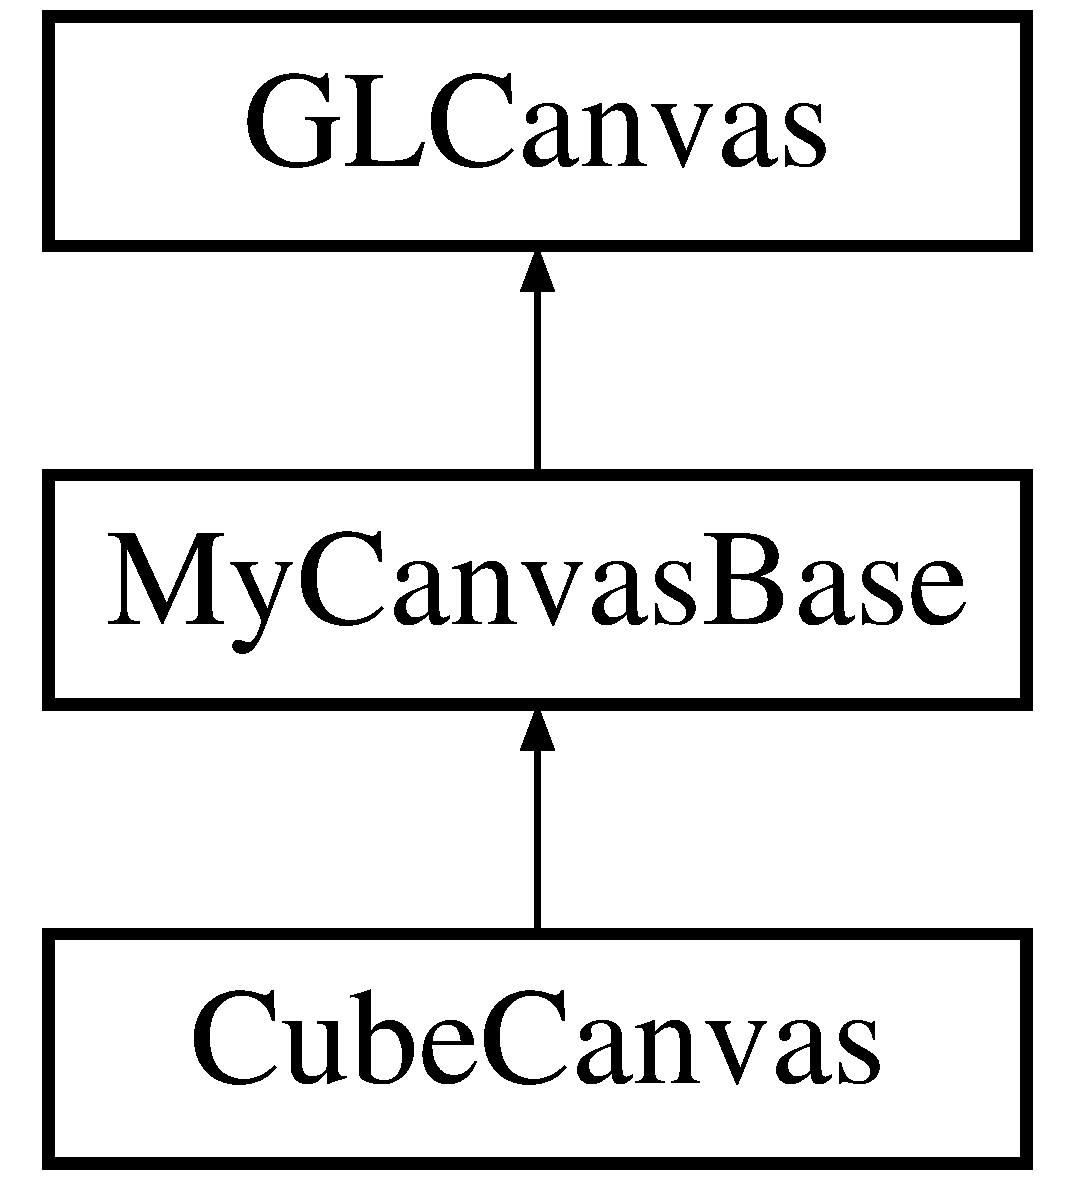
\includegraphics[height=3.000000cm]{classarbitros_ahrs_1_1_cube_canvas}
\end{center}
\end{figure}
\subsection*{Public Member Functions}
\begin{DoxyCompactItemize}
\item 
\hypertarget{classarbitros_ahrs_1_1_cube_canvas_aa5d4da6894799e330c531fcff2320723}{def {\bfseries Init\-G\-L}}\label{classarbitros_ahrs_1_1_cube_canvas_aa5d4da6894799e330c531fcff2320723}

\item 
\hypertarget{classarbitros_ahrs_1_1_cube_canvas_a06264628fa709c57ac53fe3f63080317}{def {\bfseries On\-Draw}}\label{classarbitros_ahrs_1_1_cube_canvas_a06264628fa709c57ac53fe3f63080317}

\end{DoxyCompactItemize}
\subsection*{Data Fields}
\begin{DoxyCompactItemize}
\item 
\hypertarget{classarbitros_ahrs_1_1_cube_canvas_aa3d6656320f1a7278c0c2c7fdf07617c}{{\bfseries size}}\label{classarbitros_ahrs_1_1_cube_canvas_aa3d6656320f1a7278c0c2c7fdf07617c}

\end{DoxyCompactItemize}


The documentation for this class was generated from the following file\-:\begin{DoxyCompactItemize}
\item 
C\-:/arbitros/trunk/boards/primus/examples/ins/python/arbitros\-Ahrs.\-py\end{DoxyCompactItemize}

\hypertarget{structeeprom}{\section{eeprom Struct Reference}
\label{structeeprom}\index{eeprom@{eeprom}}
}
\subsection*{Data Fields}
\begin{DoxyCompactItemize}
\item 
\hypertarget{structeeprom_a2a1d740f7d94119ed71fa71ac11fe71f}{uint8\-\_\-t {\bfseries c\-\_\-user\-Id}}\label{structeeprom_a2a1d740f7d94119ed71fa71ac11fe71f}

\item 
\hypertarget{structeeprom_a165d1da4013945e4e6a1a8b2f3a84349}{uint8\-\_\-t {\bfseries c\-\_\-start\-Page\-Addr}}\label{structeeprom_a165d1da4013945e4e6a1a8b2f3a84349}

\item 
\hypertarget{structeeprom_a979ea932d34fda8eaf1b1216fd4d0d9a}{int16\-\_\-t {\bfseries s\-\_\-size\-Bytes}}\label{structeeprom_a979ea932d34fda8eaf1b1216fd4d0d9a}

\item 
\hypertarget{structeeprom_ae9defadc0b153c6091d7f23bcb95ef22}{struct \hyperlink{structeeprom}{eeprom} $\ast$ {\bfseries pt\-\_\-next}}\label{structeeprom_ae9defadc0b153c6091d7f23bcb95ef22}

\item 
\hypertarget{structeeprom_a3aecd98f8fcd3681ab58dcc5042658ad}{struct \hyperlink{structeeprom}{eeprom} $\ast$ {\bfseries pt\-\_\-prev}}\label{structeeprom_a3aecd98f8fcd3681ab58dcc5042658ad}

\end{DoxyCompactItemize}


The documentation for this struct was generated from the following file\-:\begin{DoxyCompactItemize}
\item 
C\-:/arbitros/trunk/utilities/source/xmega128\-A1/utl\-\_\-eeprom.\-c\end{DoxyCompactItemize}

\hypertarget{structlist_link}{\section{list\-Link Struct Reference}
\label{structlist_link}\index{list\-Link@{list\-Link}}
}
\subsection*{Data Fields}
\begin{DoxyCompactItemize}
\item 
\hypertarget{structlist_link_ab34ba6b213f1b6be9b8fbb9ed5ea50de}{void $\ast$ {\bfseries pv\-\_\-element}}\label{structlist_link_ab34ba6b213f1b6be9b8fbb9ed5ea50de}

\item 
\hypertarget{structlist_link_aad2e96fd3a0b75e3a7d314eabb08bc2b}{uint16\-\_\-t {\bfseries s\-\_\-element\-Size\-Bytes}}\label{structlist_link_aad2e96fd3a0b75e3a7d314eabb08bc2b}

\item 
\hypertarget{structlist_link_ab6a669366106c0a82a7ff6b2aed5c915}{uint16\-\_\-t {\bfseries s\-\_\-cont\-Addr}}\label{structlist_link_ab6a669366106c0a82a7ff6b2aed5c915}

\item 
\hypertarget{structlist_link_a6904a7252c37d795af502f166930283a}{uint16\-\_\-t {\bfseries s\-\_\-link\-Size\-Bytes}}\label{structlist_link_a6904a7252c37d795af502f166930283a}

\item 
\hypertarget{structlist_link_a27153ba7aa91e597195e2459a18d9bbb}{struct \hyperlink{structlist_link}{list\-Link} $\ast$ {\bfseries pt\-\_\-next}}\label{structlist_link_a27153ba7aa91e597195e2459a18d9bbb}

\item 
\hypertarget{structlist_link_acbd20e20dbad288dc19aa04f85501688}{struct \hyperlink{structlist_link}{list\-Link} $\ast$ {\bfseries pt\-\_\-prev}}\label{structlist_link_acbd20e20dbad288dc19aa04f85501688}

\end{DoxyCompactItemize}


The documentation for this struct was generated from the following file\-:\begin{DoxyCompactItemize}
\item 
C\-:/arbitros/trunk/utilities/headers/common/utl\-\_\-linkedlist.\-h\end{DoxyCompactItemize}

\hypertarget{classarbitros_ahrs_1_1_main_window}{\section{Main\-Window Class Reference}
\label{classarbitros_ahrs_1_1_main_window}\index{Main\-Window@{Main\-Window}}
}
Inheritance diagram for Main\-Window\-:\begin{figure}[H]
\begin{center}
\leavevmode
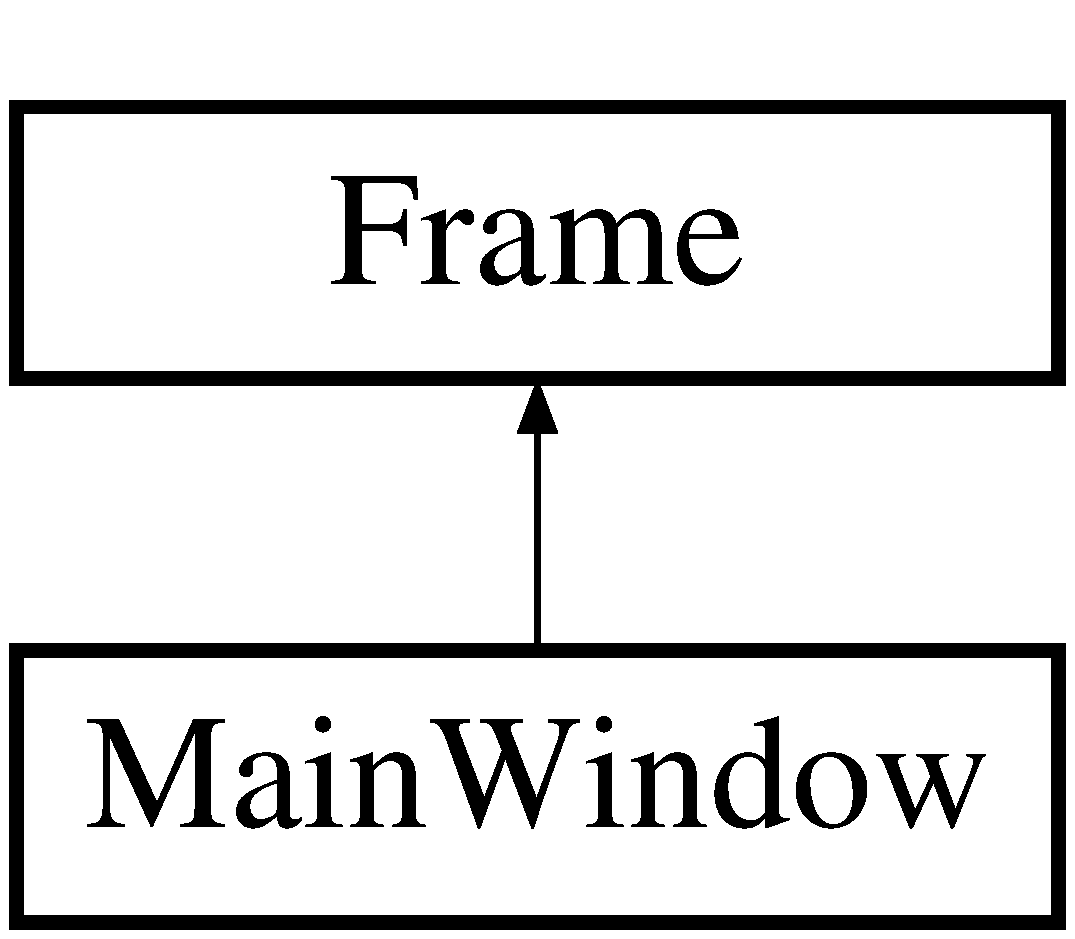
\includegraphics[height=2.000000cm]{classarbitros_ahrs_1_1_main_window}
\end{center}
\end{figure}


The documentation for this class was generated from the following file\-:\begin{DoxyCompactItemize}
\item 
C\-:/arbitros/trunk/boards/primus/examples/ins/python/arbitros\-Ahrs.\-py\end{DoxyCompactItemize}

\hypertarget{classarbitros_ahrs_1_1_my_canvas_base}{\section{My\-Canvas\-Base Class Reference}
\label{classarbitros_ahrs_1_1_my_canvas_base}\index{My\-Canvas\-Base@{My\-Canvas\-Base}}
}
Inheritance diagram for My\-Canvas\-Base\-:\begin{figure}[H]
\begin{center}
\leavevmode
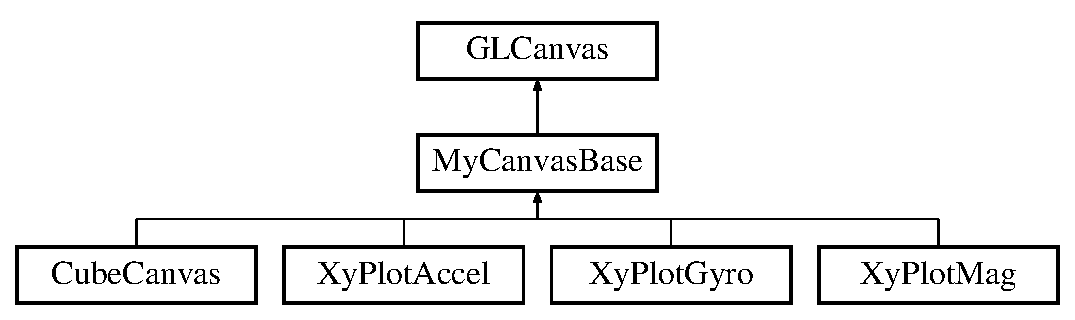
\includegraphics[height=3.000000cm]{classarbitros_ahrs_1_1_my_canvas_base}
\end{center}
\end{figure}


The documentation for this class was generated from the following file\-:\begin{DoxyCompactItemize}
\item 
C\-:/arbitros/trunk/boards/primus/examples/ins/python/arbitros\-Ahrs.\-py\end{DoxyCompactItemize}

\hypertarget{structt__accel_dev}{\section{t\-\_\-accel\-Dev Struct Reference}
\label{structt__accel_dev}\index{t\-\_\-accel\-Dev@{t\-\_\-accel\-Dev}}
}
\subsection*{Data Fields}
\begin{DoxyCompactItemize}
\item 
\hypertarget{structt__accel_dev_ad7daca491dc2ace488c7fd26eee4c5e9}{int16\-\_\-t {\bfseries as\-\_\-\-R} \mbox{[}3\mbox{]}\mbox{[}3\mbox{]}}\label{structt__accel_dev_ad7daca491dc2ace488c7fd26eee4c5e9}

\item 
\hypertarget{structt__accel_dev_a090c73eef857227542434acce66453fd}{int16\-\_\-t {\bfseries as\-\_\-scale} \mbox{[}3\mbox{]}}\label{structt__accel_dev_a090c73eef857227542434acce66453fd}

\item 
\hypertarget{structt__accel_dev_ab09e9163fcbdd1f8df41f93844da2d68}{int16\-\_\-t {\bfseries as\-\_\-bias} \mbox{[}3\mbox{]}}\label{structt__accel_dev_ab09e9163fcbdd1f8df41f93844da2d68}

\item 
\hypertarget{structt__accel_dev_a7a5f0992351377907af87663257e1957}{int16\-\_\-t {\bfseries s\-\_\-cal\-Gravity}}\label{structt__accel_dev_a7a5f0992351377907af87663257e1957}

\item 
\hypertarget{structt__accel_dev_a5b8c77544b001e373f59189f0fbe6878}{t\-\_\-ins\-Cal\-Status {\bfseries t\-\_\-cal}}\label{structt__accel_dev_a5b8c77544b001e373f59189f0fbe6878}

\item 
\hypertarget{structt__accel_dev_a9b8095efdf7231ca020b21028fdd1916}{int16\-\_\-t {\bfseries s\-\_\-avr\-Spec\-Force}}\label{structt__accel_dev_a9b8095efdf7231ca020b21028fdd1916}

\end{DoxyCompactItemize}


The documentation for this struct was generated from the following file\-:\begin{DoxyCompactItemize}
\item 
C\-:/arbitros/trunk/drivers/source/drv\-\_\-ins.\-c\end{DoxyCompactItemize}

\hypertarget{structt__adc_chan_conf}{\section{t\-\_\-adc\-Chan\-Conf Struct Reference}
\label{structt__adc_chan_conf}\index{t\-\_\-adc\-Chan\-Conf@{t\-\_\-adc\-Chan\-Conf}}
}
\subsection*{Data Fields}
\begin{DoxyCompactItemize}
\item 
\hypertarget{structt__adc_chan_conf_a7cc030ac8f699366c00c39ecf374c329}{uint8\-\_\-t {\bfseries c\-\_\-pos\-Pin}}\label{structt__adc_chan_conf_a7cc030ac8f699366c00c39ecf374c329}

\item 
\hypertarget{structt__adc_chan_conf_a91b82012399e28a2cbd397398946a86f}{uint8\-\_\-t {\bfseries c\-\_\-neg\-Pin}}\label{structt__adc_chan_conf_a91b82012399e28a2cbd397398946a86f}

\item 
\hypertarget{structt__adc_chan_conf_abdb8311beea49b3bd822f1b98dfc08c3}{t\-\_\-input\-Mode {\bfseries t\-\_\-in\-Mode}}\label{structt__adc_chan_conf_abdb8311beea49b3bd822f1b98dfc08c3}

\item 
\hypertarget{structt__adc_chan_conf_a142ba07e114d05a086296ac009a4bcf5}{t\-\_\-diff\-Gain {\bfseries t\-\_\-gain}}\label{structt__adc_chan_conf_a142ba07e114d05a086296ac009a4bcf5}

\item 
\hypertarget{structt__adc_chan_conf_aeb813e3541a49409efebed0794946b60}{bool {\bfseries b\-\_\-enable\-Int}}\label{structt__adc_chan_conf_aeb813e3541a49409efebed0794946b60}

\item 
\hypertarget{structt__adc_chan_conf_abf60fe278e4ec7ed455a81f8d270357a}{void($\ast$ {\bfseries pf\-\_\-fun\-Ptr} )(int16\-\_\-t s\-\_\-sample)}\label{structt__adc_chan_conf_abf60fe278e4ec7ed455a81f8d270357a}

\end{DoxyCompactItemize}


The documentation for this struct was generated from the following file\-:\begin{DoxyCompactItemize}
\item 
C\-:/arbitros/trunk/utilities/headers/xmega128\-A1/utl\-\_\-adc.\-h\end{DoxyCompactItemize}

\hypertarget{structt__adc_mod_conf}{\section{t\-\_\-adc\-Mod\-Conf Struct Reference}
\label{structt__adc_mod_conf}\index{t\-\_\-adc\-Mod\-Conf@{t\-\_\-adc\-Mod\-Conf}}
}
\subsection*{Data Fields}
\begin{DoxyCompactItemize}
\item 
\hypertarget{structt__adc_mod_conf_aa15f0849345837f8f5a2b3acea398315}{t\-\_\-conv\-Mode {\bfseries t\-\_\-mode}}\label{structt__adc_mod_conf_aa15f0849345837f8f5a2b3acea398315}

\item 
\hypertarget{structt__adc_mod_conf_a24a483c3b37199a23881efb390da0a1f}{t\-\_\-mes\-Resolution {\bfseries t\-\_\-res}}\label{structt__adc_mod_conf_a24a483c3b37199a23881efb390da0a1f}

\item 
\hypertarget{structt__adc_mod_conf_ab1afe935ff844b12f7a1bff1a0d562b6}{t\-\_\-ref\-Voltage {\bfseries t\-\_\-ref}}\label{structt__adc_mod_conf_ab1afe935ff844b12f7a1bff1a0d562b6}

\item 
\hypertarget{structt__adc_mod_conf_ade8770475a77e637a3db85be06757c6c}{t\-\_\-ref\-Clock {\bfseries t\-\_\-clock}}\label{structt__adc_mod_conf_ade8770475a77e637a3db85be06757c6c}

\end{DoxyCompactItemize}


The documentation for this struct was generated from the following file\-:\begin{DoxyCompactItemize}
\item 
C\-:/arbitros/trunk/utilities/headers/xmega128\-A1/utl\-\_\-adc.\-h\end{DoxyCompactItemize}

\hypertarget{structt__arb_comm_dev}{\section{t\-\_\-arb\-Comm\-Dev Struct Reference}
\label{structt__arb_comm_dev}\index{t\-\_\-arb\-Comm\-Dev@{t\-\_\-arb\-Comm\-Dev}}
}
\subsection*{Data Fields}
\begin{DoxyCompactItemize}
\item 
\hypertarget{structt__arb_comm_dev_a6c668c5c6ef7ecd4aa0eeca1dc3352cf}{t\-\_\-\-S\-E\-M\-H\-A\-N\-D\-L\-E {\bfseries t\-\_\-rx\-Mutex}}\label{structt__arb_comm_dev_a6c668c5c6ef7ecd4aa0eeca1dc3352cf}

\item 
\hypertarget{structt__arb_comm_dev_a17abeacecc1a41425fc9fd04a89e026e}{t\-\_\-\-S\-E\-M\-H\-A\-N\-D\-L\-E {\bfseries t\-\_\-tx\-Mutex}}\label{structt__arb_comm_dev_a17abeacecc1a41425fc9fd04a89e026e}

\item 
\hypertarget{structt__arb_comm_dev_abfbc70e94616edab7b4177058a7f188d}{t\-\_\-\-B\-U\-F\-F\-H\-A\-N\-D\-L\-E {\bfseries t\-\_\-rx\-Buffer}}\label{structt__arb_comm_dev_abfbc70e94616edab7b4177058a7f188d}

\item 
\hypertarget{structt__arb_comm_dev_a65907c8d88006e5cdc5e6b18eb4606ba}{uint8\-\_\-t {\bfseries c\-\_\-num\-Users}}\label{structt__arb_comm_dev_a65907c8d88006e5cdc5e6b18eb4606ba}

\item 
\hypertarget{structt__arb_comm_dev_adff9fcc9b301fd4d7521fb37d7490034}{t\-\_\-\-U\-A\-R\-T\-H\-N\-D\-L {\bfseries t\-\_\-u\-Handle}}\label{structt__arb_comm_dev_adff9fcc9b301fd4d7521fb37d7490034}

\end{DoxyCompactItemize}


The documentation for this struct was generated from the following file\-:\begin{DoxyCompactItemize}
\item 
C\-:/arbitros/trunk/drivers/source/drv\-\_\-arb\-Comm.\-c\end{DoxyCompactItemize}

\hypertarget{structt__arb_comm_setup}{\section{t\-\_\-arb\-Comm\-Setup Struct Reference}
\label{structt__arb_comm_setup}\index{t\-\_\-arb\-Comm\-Setup@{t\-\_\-arb\-Comm\-Setup}}
}
\subsection*{Data Fields}
\begin{DoxyCompactItemize}
\item 
\hypertarget{structt__arb_comm_setup_ad3c09231d7c012199f3501b37686d955}{uint16\-\_\-t {\bfseries s\-\_\-rx\-Buff\-Size}}\label{structt__arb_comm_setup_ad3c09231d7c012199f3501b37686d955}

\item 
\hypertarget{structt__arb_comm_setup_ac316d01a82a05edc681fdfe0bac24060}{uint32\-\_\-t {\bfseries i\-\_\-baud\-Rate}}\label{structt__arb_comm_setup_ac316d01a82a05edc681fdfe0bac24060}

\item 
\hypertarget{structt__arb_comm_setup_a40f57779b05162e1cea2635c18c6dad9}{uint8\-\_\-t {\bfseries c\-\_\-uart\-Id}}\label{structt__arb_comm_setup_a40f57779b05162e1cea2635c18c6dad9}

\item 
\hypertarget{structt__arb_comm_setup_afba9106eb2fa769623759a1b529f884e}{uint8\-\_\-t {\bfseries c\-\_\-major\-Num}}\label{structt__arb_comm_setup_afba9106eb2fa769623759a1b529f884e}

\end{DoxyCompactItemize}


The documentation for this struct was generated from the following file\-:\begin{DoxyCompactItemize}
\item 
C\-:/arbitros/trunk/drivers/headers/drv\-\_\-arb\-Comm.\-h\end{DoxyCompactItemize}

\hypertarget{structt__buffer_handle}{\section{t\-\_\-buffer\-Handle Struct Reference}
\label{structt__buffer_handle}\index{t\-\_\-buffer\-Handle@{t\-\_\-buffer\-Handle}}
}
\subsection*{Data Fields}
\begin{DoxyCompactItemize}
\item 
\hypertarget{structt__buffer_handle_a6741870caf9385528b6cc1783d09c355}{int16\-\_\-t {\bfseries s\-\_\-wr\-Index}}\label{structt__buffer_handle_a6741870caf9385528b6cc1783d09c355}

\item 
\hypertarget{structt__buffer_handle_a9cd61a0c9822803598f10965ba2437f7}{int16\-\_\-t {\bfseries s\-\_\-rd\-Index}}\label{structt__buffer_handle_a9cd61a0c9822803598f10965ba2437f7}

\item 
\hypertarget{structt__buffer_handle_aee0d3a41a9ff196c45450679f40f71a0}{int16\-\_\-t {\bfseries s\-\_\-fill\-Count}}\label{structt__buffer_handle_aee0d3a41a9ff196c45450679f40f71a0}

\item 
\hypertarget{structt__buffer_handle_a0550159437736c023c9301562223043c}{uint16\-\_\-t {\bfseries s\-\_\-size\-Bytes}}\label{structt__buffer_handle_a0550159437736c023c9301562223043c}

\item 
\hypertarget{structt__buffer_handle_a3fa52699622cd2b4c13e1d546970b25f}{int8\-\_\-t $\ast$ {\bfseries pc\-\_\-buffer}}\label{structt__buffer_handle_a3fa52699622cd2b4c13e1d546970b25f}

\end{DoxyCompactItemize}


The documentation for this struct was generated from the following file\-:\begin{DoxyCompactItemize}
\item 
C\-:/arbitros/trunk/utilities/source/common/utl\-\_\-buffer.\-c\end{DoxyCompactItemize}

\hypertarget{structt__card_info_msg}{\section{t\-\_\-card\-Info\-Msg Struct Reference}
\label{structt__card_info_msg}\index{t\-\_\-card\-Info\-Msg@{t\-\_\-card\-Info\-Msg}}
}
\subsection*{Data Fields}
\begin{DoxyCompactItemize}
\item 
\hypertarget{structt__card_info_msg_ad3bb35301ef17fc663c93a81c374cf78}{uint8\-\_\-t {\bfseries c\-\_\-card\-Type}}\label{structt__card_info_msg_ad3bb35301ef17fc663c93a81c374cf78}

\end{DoxyCompactItemize}


The documentation for this struct was generated from the following file\-:\begin{DoxyCompactItemize}
\item 
C\-:/arbitros/trunk/drivers/headers/drv\-\_\-sd.\-h\end{DoxyCompactItemize}

\hypertarget{structt__chan_handle}{\section{t\-\_\-chan\-Handle Struct Reference}
\label{structt__chan_handle}\index{t\-\_\-chan\-Handle@{t\-\_\-chan\-Handle}}
}
\subsection*{Data Fields}
\begin{DoxyCompactItemize}
\item 
\hypertarget{structt__chan_handle_a6ac807ac205ab76b1bf99317ca765bdf}{t\-\_\-adc\-Module\-Id {\bfseries t\-\_\-module}}\label{structt__chan_handle_a6ac807ac205ab76b1bf99317ca765bdf}

\item 
\hypertarget{structt__chan_handle_a763f43b20d35ad0faecf3756080b4d80}{t\-\_\-chan\-Id {\bfseries t\-\_\-id}}\label{structt__chan_handle_a763f43b20d35ad0faecf3756080b4d80}

\item 
\hypertarget{structt__chan_handle_a4e1d5aa0bdda779cf36aa45919f7a12a}{A\-D\-C\-\_\-\-C\-H\-\_\-t $\ast$ {\bfseries pt\-\_\-chan}}\label{structt__chan_handle_a4e1d5aa0bdda779cf36aa45919f7a12a}

\item 
\hypertarget{structt__chan_handle_a4362e3180de16ca1aa9d856270c66c98}{int16\-\_\-t {\bfseries s\-\_\-adc\-Sample}}\label{structt__chan_handle_a4362e3180de16ca1aa9d856270c66c98}

\item 
\hypertarget{structt__chan_handle_abf60fe278e4ec7ed455a81f8d270357a}{void($\ast$ {\bfseries pf\-\_\-fun\-Ptr} )(int16\-\_\-t s\-\_\-sample)}\label{structt__chan_handle_abf60fe278e4ec7ed455a81f8d270357a}

\end{DoxyCompactItemize}


The documentation for this struct was generated from the following file\-:\begin{DoxyCompactItemize}
\item 
C\-:/arbitros/trunk/utilities/source/xmega128\-A1/utl\-\_\-adc.\-c\end{DoxyCompactItemize}

\hypertarget{structt__clocks}{\section{t\-\_\-clocks Struct Reference}
\label{structt__clocks}\index{t\-\_\-clocks@{t\-\_\-clocks}}
}
\subsection*{Data Fields}
\begin{DoxyCompactItemize}
\item 
\hypertarget{structt__clocks_a50c91a72dfb71a07efe14f43fbed63c6}{uint32\-\_\-t {\bfseries i\-\_\-cpu\-Clock}}\label{structt__clocks_a50c91a72dfb71a07efe14f43fbed63c6}

\end{DoxyCompactItemize}


The documentation for this struct was generated from the following file\-:\begin{DoxyCompactItemize}
\item 
C\-:/arbitros/trunk/utilities/source/xmega128\-A1/utl\-\_\-clocks.\-c\end{DoxyCompactItemize}

\hypertarget{structt__console_dev}{\section{t\-\_\-console\-Dev Struct Reference}
\label{structt__console_dev}\index{t\-\_\-console\-Dev@{t\-\_\-console\-Dev}}
}
\subsection*{Data Fields}
\begin{DoxyCompactItemize}
\item 
\hypertarget{structt__console_dev_a6c668c5c6ef7ecd4aa0eeca1dc3352cf}{t\-\_\-\-S\-E\-M\-H\-A\-N\-D\-L\-E {\bfseries t\-\_\-rx\-Mutex}}\label{structt__console_dev_a6c668c5c6ef7ecd4aa0eeca1dc3352cf}

\item 
\hypertarget{structt__console_dev_a17abeacecc1a41425fc9fd04a89e026e}{t\-\_\-\-S\-E\-M\-H\-A\-N\-D\-L\-E {\bfseries t\-\_\-tx\-Mutex}}\label{structt__console_dev_a17abeacecc1a41425fc9fd04a89e026e}

\item 
\hypertarget{structt__console_dev_aedc039854e5cfc913eb025a5b4d8e744}{t\-\_\-\-S\-E\-M\-H\-A\-N\-D\-L\-E {\bfseries t\-\_\-rx\-Blocking\-Sem}}\label{structt__console_dev_aedc039854e5cfc913eb025a5b4d8e744}

\item 
\hypertarget{structt__console_dev_abfbc70e94616edab7b4177058a7f188d}{t\-\_\-\-B\-U\-F\-F\-H\-A\-N\-D\-L\-E {\bfseries t\-\_\-rx\-Buffer}}\label{structt__console_dev_abfbc70e94616edab7b4177058a7f188d}

\item 
\hypertarget{structt__console_dev_a65907c8d88006e5cdc5e6b18eb4606ba}{uint8\-\_\-t {\bfseries c\-\_\-num\-Users}}\label{structt__console_dev_a65907c8d88006e5cdc5e6b18eb4606ba}

\item 
\hypertarget{structt__console_dev_adff9fcc9b301fd4d7521fb37d7490034}{t\-\_\-\-U\-A\-R\-T\-H\-N\-D\-L {\bfseries t\-\_\-u\-Handle}}\label{structt__console_dev_adff9fcc9b301fd4d7521fb37d7490034}

\item 
\hypertarget{structt__console_dev_a3462e997b9d47e7d2ec8f1144035fbf0}{bool {\bfseries b\-\_\-rx\-Active}}\label{structt__console_dev_a3462e997b9d47e7d2ec8f1144035fbf0}

\item 
\hypertarget{structt__console_dev_a438be64e1e5f557076bc94c2c50e28d1}{int8\-\_\-t {\bfseries c\-\_\-cmd\-Prompt\-Color}}\label{structt__console_dev_a438be64e1e5f557076bc94c2c50e28d1}

\item 
\hypertarget{structt__console_dev_a062d373a04ec81e7297f2b0fc1f91d07}{int8\-\_\-t {\bfseries c\-\_\-fg\-Color}}\label{structt__console_dev_a062d373a04ec81e7297f2b0fc1f91d07}

\item 
\hypertarget{structt__console_dev_aec8faf14e3ad2366f022691be3587617}{char {\bfseries ac\-\_\-dir\-Name} \mbox{[}C\-O\-N\-S\-O\-L\-E\-\_\-\-M\-A\-X\-\_\-\-T\-O\-K\-E\-N\-\_\-\-S\-I\-Z\-E\mbox{]}}\label{structt__console_dev_aec8faf14e3ad2366f022691be3587617}

\end{DoxyCompactItemize}


The documentation for this struct was generated from the following file\-:\begin{DoxyCompactItemize}
\item 
C\-:/arbitros/trunk/drivers/source/drv\-\_\-console.\-c\end{DoxyCompactItemize}

\hypertarget{structt__console_object}{\section{t\-\_\-console\-Object Struct Reference}
\label{structt__console_object}\index{t\-\_\-console\-Object@{t\-\_\-console\-Object}}
}


Grouping of objects commonly used across all functions within this file.  


\subsection*{Data Fields}
\begin{DoxyCompactItemize}
\item 
t\-\_\-\-T\-H\-R\-D\-H\-A\-N\-D\-L\-E \hyperlink{structt__console_object_ae0eceac7658ed204c517d618961e5cd9}{t\-\_\-console\-Thread}
\item 
t\-\_\-\-D\-E\-V\-H\-A\-N\-D\-L\-E \hyperlink{structt__console_object_a6f9d3d1fa28b532e16089830ab73c3b6}{t\-\_\-console\-Hndl}
\item 
t\-\_\-\-D\-E\-V\-H\-A\-N\-D\-L\-E \hyperlink{structt__console_object_aaabb9b990f986cd929e22cd0da9586f1}{t\-\_\-sd\-Hndl}
\item 
bool($\ast$ \hyperlink{structt__console_object_a43c5369489e99b24653bd0b0ff0e77e0}{pf\-\_\-fun\-Ptr} )(t\-\_\-\-D\-E\-V\-H\-A\-N\-D\-L\-E \hyperlink{structt__console_object_a6f9d3d1fa28b532e16089830ab73c3b6}{t\-\_\-console\-Hndl}, int8\-\_\-t $\ast$pc\-\_\-buff, \hyperlink{structt__console_tok_hndl}{t\-\_\-console\-Tok\-Hndl} $\ast$pt\-\_\-tok\-Hndl)
\end{DoxyCompactItemize}


\subsection{Detailed Description}
Grouping of objects commonly used across all functions within this file. 

\subsection{Field Documentation}
\hypertarget{structt__console_object_a43c5369489e99b24653bd0b0ff0e77e0}{\index{t\-\_\-console\-Object@{t\-\_\-console\-Object}!pf\-\_\-fun\-Ptr@{pf\-\_\-fun\-Ptr}}
\index{pf\-\_\-fun\-Ptr@{pf\-\_\-fun\-Ptr}!t_consoleObject@{t\-\_\-console\-Object}}
\subsubsection[{pf\-\_\-fun\-Ptr}]{\setlength{\rightskip}{0pt plus 5cm}bool($\ast$ pf\-\_\-fun\-Ptr)(t\-\_\-\-D\-E\-V\-H\-A\-N\-D\-L\-E {\bf t\-\_\-console\-Hndl}, int8\-\_\-t $\ast$pc\-\_\-buff, {\bf t\-\_\-console\-Tok\-Hndl} $\ast$pt\-\_\-tok\-Hndl)}}\label{structt__console_object_a43c5369489e99b24653bd0b0ff0e77e0}
Pointer to the user-\/space console handler configured during module initialization (\#arb\-\_\-console\-Init). The console thread (\hyperlink{arb__console_8c_a53daff761c655e05e651b375d95d6309}{arb\-\_\-console}) passes control to this function after determining that a command (entered over the terminal) is not part of the Arbitros basic kernel command set. \hypertarget{structt__console_object_a6f9d3d1fa28b532e16089830ab73c3b6}{\index{t\-\_\-console\-Object@{t\-\_\-console\-Object}!t\-\_\-console\-Hndl@{t\-\_\-console\-Hndl}}
\index{t\-\_\-console\-Hndl@{t\-\_\-console\-Hndl}!t_consoleObject@{t\-\_\-console\-Object}}
\subsubsection[{t\-\_\-console\-Hndl}]{\setlength{\rightskip}{0pt plus 5cm}t\-\_\-\-D\-E\-V\-H\-A\-N\-D\-L\-E t\-\_\-console\-Hndl}}\label{structt__console_object_a6f9d3d1fa28b532e16089830ab73c3b6}
Handle to the console thread created during module initialization (\#arb\-\_\-console\-Init). Handles are the primary mechanism for linking a thread (i.\-e. \hyperlink{arb__console_8c_a53daff761c655e05e651b375d95d6309}{arb\-\_\-console})--through the kernel--to the particular device driver its trying to access. \hypertarget{structt__console_object_ae0eceac7658ed204c517d618961e5cd9}{\index{t\-\_\-console\-Object@{t\-\_\-console\-Object}!t\-\_\-console\-Thread@{t\-\_\-console\-Thread}}
\index{t\-\_\-console\-Thread@{t\-\_\-console\-Thread}!t_consoleObject@{t\-\_\-console\-Object}}
\subsubsection[{t\-\_\-console\-Thread}]{\setlength{\rightskip}{0pt plus 5cm}t\-\_\-\-T\-H\-R\-D\-H\-A\-N\-D\-L\-E t\-\_\-console\-Thread}}\label{structt__console_object_ae0eceac7658ed204c517d618961e5cd9}
Handle to the console thread created during module initialization (\#arb\-\_\-console\-Init). \hypertarget{structt__console_object_aaabb9b990f986cd929e22cd0da9586f1}{\index{t\-\_\-console\-Object@{t\-\_\-console\-Object}!t\-\_\-sd\-Hndl@{t\-\_\-sd\-Hndl}}
\index{t\-\_\-sd\-Hndl@{t\-\_\-sd\-Hndl}!t_consoleObject@{t\-\_\-console\-Object}}
\subsubsection[{t\-\_\-sd\-Hndl}]{\setlength{\rightskip}{0pt plus 5cm}t\-\_\-\-D\-E\-V\-H\-A\-N\-D\-L\-E t\-\_\-sd\-Hndl}}\label{structt__console_object_aaabb9b990f986cd929e22cd0da9586f1}
Handle to the fat32 S\-D card driver created during module initialization (\#arb\-\_\-console\-Init). This handle provides a way of exposing file system functionality--such as directory searching, file deletion, and reading the contents of a file--to an external user via the terminal command window by way of the \hyperlink{arb__console_8c_a53daff761c655e05e651b375d95d6309}{arb\-\_\-console} thread. 

The documentation for this struct was generated from the following files\-:\begin{DoxyCompactItemize}
\item 
C\-:/arbitros/trunk/rtos/source/common/\hyperlink{arb__console_8c}{arb\-\_\-console.\-c}\item 
C\-:/arbitros/trunk/boards/primus/examples/ins/source/usr\-\_\-console.\-c\end{DoxyCompactItemize}

\hypertarget{structt__console_setup}{\section{t\-\_\-console\-Setup Struct Reference}
\label{structt__console_setup}\index{t\-\_\-console\-Setup@{t\-\_\-console\-Setup}}
}
\subsection*{Data Fields}
\begin{DoxyCompactItemize}
\item 
\hypertarget{structt__console_setup_ac316d01a82a05edc681fdfe0bac24060}{uint32\-\_\-t {\bfseries i\-\_\-baud\-Rate}}\label{structt__console_setup_ac316d01a82a05edc681fdfe0bac24060}

\item 
\hypertarget{structt__console_setup_a40f57779b05162e1cea2635c18c6dad9}{uint8\-\_\-t {\bfseries c\-\_\-uart\-Id}}\label{structt__console_setup_a40f57779b05162e1cea2635c18c6dad9}

\item 
\hypertarget{structt__console_setup_afba9106eb2fa769623759a1b529f884e}{uint8\-\_\-t {\bfseries c\-\_\-major\-Num}}\label{structt__console_setup_afba9106eb2fa769623759a1b529f884e}

\end{DoxyCompactItemize}


The documentation for this struct was generated from the following file\-:\begin{DoxyCompactItemize}
\item 
C\-:/arbitros/trunk/drivers/headers/drv\-\_\-console.\-h\end{DoxyCompactItemize}

\hypertarget{structt__console_tok_hndl}{\section{t\-\_\-console\-Tok\-Hndl Struct Reference}
\label{structt__console_tok_hndl}\index{t\-\_\-console\-Tok\-Hndl@{t\-\_\-console\-Tok\-Hndl}}
}
\subsection*{Data Fields}
\begin{DoxyCompactItemize}
\item 
\hypertarget{structt__console_tok_hndl_a5da4ae36c0c86f4e292040dcfa814fad}{int8\-\_\-t {\bfseries ac\-\_\-tok} \mbox{[}C\-O\-N\-S\-O\-L\-E\-\_\-\-M\-A\-X\-\_\-\-T\-O\-K\-E\-N\-S\mbox{]}\mbox{[}C\-O\-N\-S\-O\-L\-E\-\_\-\-M\-A\-X\-\_\-\-T\-O\-K\-E\-N\-\_\-\-S\-I\-Z\-E\mbox{]}}\label{structt__console_tok_hndl_a5da4ae36c0c86f4e292040dcfa814fad}

\item 
\hypertarget{structt__console_tok_hndl_a143bcd8f046c8817cfe6577cf473883e}{uint8\-\_\-t {\bfseries c\-\_\-num\-Tokens}}\label{structt__console_tok_hndl_a143bcd8f046c8817cfe6577cf473883e}

\end{DoxyCompactItemize}


The documentation for this struct was generated from the following file\-:\begin{DoxyCompactItemize}
\item 
C\-:/arbitros/trunk/drivers/headers/drv\-\_\-console.\-h\end{DoxyCompactItemize}

\hypertarget{structt__curs_pos}{\section{t\-\_\-curs\-Pos Struct Reference}
\label{structt__curs_pos}\index{t\-\_\-curs\-Pos@{t\-\_\-curs\-Pos}}
}
\subsection*{Data Fields}
\begin{DoxyCompactItemize}
\item 
\hypertarget{structt__curs_pos_a6f99a6b7388142dd31b55ef00a2d9386}{uint8\-\_\-t {\bfseries c\-\_\-row}}\label{structt__curs_pos_a6f99a6b7388142dd31b55ef00a2d9386}

\item 
\hypertarget{structt__curs_pos_aeb304f930f2ea1a47266e1f85883568f}{uint8\-\_\-t {\bfseries c\-\_\-col}}\label{structt__curs_pos_aeb304f930f2ea1a47266e1f85883568f}

\end{DoxyCompactItemize}


The documentation for this struct was generated from the following file\-:\begin{DoxyCompactItemize}
\item 
C\-:/arbitros/trunk/drivers/headers/drv\-\_\-lcd.\-h\end{DoxyCompactItemize}

\hypertarget{structt__cust_char}{\section{t\-\_\-cust\-Char Struct Reference}
\label{structt__cust_char}\index{t\-\_\-cust\-Char@{t\-\_\-cust\-Char}}
}
\subsection*{Data Fields}
\begin{DoxyCompactItemize}
\item 
\hypertarget{structt__cust_char_a8c6c00ab3761d45720e9bcdf9f08e624}{uint8\-\_\-t {\bfseries c\-\_\-address}}\label{structt__cust_char_a8c6c00ab3761d45720e9bcdf9f08e624}

\item 
\hypertarget{structt__cust_char_a38157a301f42fce16b88e81decdf74c3}{uint8\-\_\-t {\bfseries ac\-\_\-bit\-Map} \mbox{[}8\mbox{]}}\label{structt__cust_char_a38157a301f42fce16b88e81decdf74c3}

\end{DoxyCompactItemize}


The documentation for this struct was generated from the following file\-:\begin{DoxyCompactItemize}
\item 
C\-:/arbitros/trunk/drivers/headers/drv\-\_\-lcd.\-h\end{DoxyCompactItemize}

\hypertarget{structt__dev_handle}{\section{t\-\_\-dev\-Handle Struct Reference}
\label{structt__dev_handle}\index{t\-\_\-dev\-Handle@{t\-\_\-dev\-Handle}}
}
\subsection*{Data Fields}
\begin{DoxyCompactItemize}
\item 
\hypertarget{structt__dev_handle_a9165a740126b0b9b05baca4031068799}{\hyperlink{structt__device}{t\-\_\-device} $\ast$ {\bfseries pt\-\_\-dev}}\label{structt__dev_handle_a9165a740126b0b9b05baca4031068799}

\item 
\hypertarget{structt__dev_handle_ac887556b30da2524683efe030d31a3e6}{void $\ast$ {\bfseries pv\-\_\-private\-Data}}\label{structt__dev_handle_ac887556b30da2524683efe030d31a3e6}

\item 
\hypertarget{structt__dev_handle_ac1bb37023c6646f713c7b97e109df684}{uint8\-\_\-t {\bfseries c\-\_\-flags}}\label{structt__dev_handle_ac1bb37023c6646f713c7b97e109df684}

\item 
\hypertarget{structt__dev_handle_a28fdd5ba1cfe7d7de9f98926ef3761d5}{uint32\-\_\-t {\bfseries i\-\_\-pos}}\label{structt__dev_handle_a28fdd5ba1cfe7d7de9f98926ef3761d5}

\end{DoxyCompactItemize}


The documentation for this struct was generated from the following file\-:\begin{DoxyCompactItemize}
\item 
C\-:/arbitros/trunk/rtos/headers/common/arb\-\_\-device.\-h\end{DoxyCompactItemize}

\hypertarget{structt__device}{\section{t\-\_\-device Struct Reference}
\label{structt__device}\index{t\-\_\-device@{t\-\_\-device}}
}
\subsection*{Data Fields}
\begin{DoxyCompactItemize}
\item 
\hypertarget{structt__device_a74f70bbd98091261a7b30808f07ccdd5}{t\-\_\-device\-Id {\bfseries t\-\_\-dev\-Id}}\label{structt__device_a74f70bbd98091261a7b30808f07ccdd5}

\item 
\hypertarget{structt__device_ad5f589905b569ab101984559869a4479}{int8\-\_\-t {\bfseries ac\-\_\-device\-Name} \mbox{[}M\-A\-X\-\_\-\-D\-E\-V\-I\-C\-E\-\_\-\-N\-A\-M\-E\-\_\-\-B\-Y\-T\-E\-S\mbox{]}}\label{structt__device_ad5f589905b569ab101984559869a4479}

\item 
\hypertarget{structt__device_acdad38f26daa29ea811e6107702f1222}{int8\-\_\-t {\bfseries c\-\_\-num\-Dev\-Handles}}\label{structt__device_acdad38f26daa29ea811e6107702f1222}

\item 
\hypertarget{structt__device_a6ecc95fd00e2577591ac693e90d3bb0a}{\hyperlink{structt__device_operations}{t\-\_\-device\-Operations} $\ast$ {\bfseries pt\-\_\-dev\-Ops}}\label{structt__device_a6ecc95fd00e2577591ac693e90d3bb0a}

\end{DoxyCompactItemize}


The documentation for this struct was generated from the following file\-:\begin{DoxyCompactItemize}
\item 
C\-:/arbitros/trunk/rtos/headers/common/arb\-\_\-device.\-h\end{DoxyCompactItemize}

\hypertarget{structt__device_operations}{\section{t\-\_\-device\-Operations Struct Reference}
\label{structt__device_operations}\index{t\-\_\-device\-Operations@{t\-\_\-device\-Operations}}
}
\subsection*{Data Fields}
\begin{DoxyCompactItemize}
\item 
\hypertarget{structt__device_operations_a608aaa9edd7f339d70df7bf7e8290041}{t\-\_\-error($\ast$ {\bfseries pf\-\_\-open} )(t\-\_\-\-D\-E\-V\-H\-A\-N\-D\-L\-E \hyperlink{structt__dev_handle}{t\-\_\-dev\-Handle})}\label{structt__device_operations_a608aaa9edd7f339d70df7bf7e8290041}

\item 
\hypertarget{structt__device_operations_a6ac8ee34b9e26013d6cff8239fb8d9cf}{int16\-\_\-t($\ast$ {\bfseries pf\-\_\-read} )(t\-\_\-\-D\-E\-V\-H\-A\-N\-D\-L\-E \hyperlink{structt__dev_handle}{t\-\_\-dev\-Handle}, int8\-\_\-t $\ast$pc\-\_\-buff, uint16\-\_\-t s\-\_\-size)}\label{structt__device_operations_a6ac8ee34b9e26013d6cff8239fb8d9cf}

\item 
\hypertarget{structt__device_operations_a4b6fd244d6ba3ca505decc7abd6ca694}{int16\-\_\-t($\ast$ {\bfseries pf\-\_\-write} )(t\-\_\-\-D\-E\-V\-H\-A\-N\-D\-L\-E \hyperlink{structt__dev_handle}{t\-\_\-dev\-Handle}, int8\-\_\-t $\ast$pc\-\_\-buff, uint16\-\_\-t s\-\_\-size)}\label{structt__device_operations_a4b6fd244d6ba3ca505decc7abd6ca694}

\item 
\hypertarget{structt__device_operations_a6fb0091a25b55629520172fe3d09c36b}{int32\-\_\-t($\ast$ {\bfseries pf\-\_\-ioctl} )(t\-\_\-\-D\-E\-V\-H\-A\-N\-D\-L\-E \hyperlink{structt__dev_handle}{t\-\_\-dev\-Handle}, uint16\-\_\-t s\-\_\-command, int32\-\_\-t i\-\_\-arguments)}\label{structt__device_operations_a6fb0091a25b55629520172fe3d09c36b}

\item 
\hypertarget{structt__device_operations_af7309283442f6002dc583cdbd6ff8c58}{t\-\_\-error($\ast$ {\bfseries pf\-\_\-close} )(t\-\_\-\-D\-E\-V\-H\-A\-N\-D\-L\-E \hyperlink{structt__dev_handle}{t\-\_\-dev\-Handle})}\label{structt__device_operations_af7309283442f6002dc583cdbd6ff8c58}

\end{DoxyCompactItemize}


The documentation for this struct was generated from the following file\-:\begin{DoxyCompactItemize}
\item 
C\-:/arbitros/trunk/rtos/headers/common/arb\-\_\-device.\-h\end{DoxyCompactItemize}

\hypertarget{structt__dma_chan}{\section{t\-\_\-dma\-Chan Struct Reference}
\label{structt__dma_chan}\index{t\-\_\-dma\-Chan@{t\-\_\-dma\-Chan}}
}
\subsection*{Data Fields}
\begin{DoxyCompactItemize}
\item 
\hypertarget{structt__dma_chan_a3d29e95e8f372d4d159a7ef03006e28d}{t\-\_\-dma\-Chan\-Id {\bfseries t\-\_\-id}}\label{structt__dma_chan_a3d29e95e8f372d4d159a7ef03006e28d}

\item 
\hypertarget{structt__dma_chan_a73c33a12d6cfbcd5768be5bddef10c27}{bool {\bfseries b\-\_\-valid\-Config}}\label{structt__dma_chan_a73c33a12d6cfbcd5768be5bddef10c27}

\item 
\hypertarget{structt__dma_chan_ad8de5a86599bef13c436790dfa6eacd5}{uint8\-\_\-t {\bfseries c\-\_\-int\-Count}}\label{structt__dma_chan_ad8de5a86599bef13c436790dfa6eacd5}

\item 
\hypertarget{structt__dma_chan_a504d2cb44fb982c1a280b63af3819a55}{D\-M\-A\-\_\-\-C\-H\-\_\-t $\ast$ {\bfseries pt\-\_\-dma}}\label{structt__dma_chan_a504d2cb44fb982c1a280b63af3819a55}

\end{DoxyCompactItemize}


The documentation for this struct was generated from the following file\-:\begin{DoxyCompactItemize}
\item 
C\-:/arbitros/trunk/utilities/source/xmega128\-A1/utl\-\_\-dma.\-c\end{DoxyCompactItemize}

\hypertarget{structt__dma_chan_config}{\section{t\-\_\-dma\-Chan\-Config Struct Reference}
\label{structt__dma_chan_config}\index{t\-\_\-dma\-Chan\-Config@{t\-\_\-dma\-Chan\-Config}}
}
\subsection*{Data Fields}
\begin{DoxyCompactItemize}
\item 
\hypertarget{structt__dma_chan_config_a9b0be49050c4f04aa3b5da11b8edc156}{uint32\-\_\-t $\ast$ {\bfseries pi\-\_\-src\-Address}}\label{structt__dma_chan_config_a9b0be49050c4f04aa3b5da11b8edc156}

\item 
\hypertarget{structt__dma_chan_config_abf558583c64871a15b42be688a100385}{uint32\-\_\-t $\ast$ {\bfseries pi\-\_\-dest\-Address}}\label{structt__dma_chan_config_abf558583c64871a15b42be688a100385}

\item 
\hypertarget{structt__dma_chan_config_aa87ce8a3aac536424d4b834360323d95}{t\-\_\-dma\-Address\-Direction {\bfseries t\-\_\-src\-Add\-Dir}}\label{structt__dma_chan_config_aa87ce8a3aac536424d4b834360323d95}

\item 
\hypertarget{structt__dma_chan_config_a95ac85842d9e05b693db9376f5daf6e3}{t\-\_\-dma\-Address\-Direction {\bfseries t\-\_\-dest\-Add\-Dir}}\label{structt__dma_chan_config_a95ac85842d9e05b693db9376f5daf6e3}

\item 
\hypertarget{structt__dma_chan_config_a1395f09edeb1c8ce6bf723300deafa0e}{t\-\_\-dma\-Address\-Reload {\bfseries t\-\_\-src\-Add\-Reload}}\label{structt__dma_chan_config_a1395f09edeb1c8ce6bf723300deafa0e}

\item 
\hypertarget{structt__dma_chan_config_a05afca3af0a4ccf4b202641126286d8e}{t\-\_\-dma\-Address\-Reload {\bfseries t\-\_\-dest\-Add\-Reload}}\label{structt__dma_chan_config_a05afca3af0a4ccf4b202641126286d8e}

\item 
\hypertarget{structt__dma_chan_config_a528845635bc947ad147113703a5f18db}{uint16\-\_\-t {\bfseries s\-\_\-block\-Size}}\label{structt__dma_chan_config_a528845635bc947ad147113703a5f18db}

\item 
\hypertarget{structt__dma_chan_config_a940ca43bafb4ddb696adfcf88fcf5f98}{t\-\_\-dma\-Burst\-Mode {\bfseries t\-\_\-burst\-Mode}}\label{structt__dma_chan_config_a940ca43bafb4ddb696adfcf88fcf5f98}

\item 
\hypertarget{structt__dma_chan_config_a515dce384709133623c34403a24be1b6}{t\-\_\-dma\-Transfer\-Type {\bfseries t\-\_\-transfer\-Type}}\label{structt__dma_chan_config_a515dce384709133623c34403a24be1b6}

\item 
\hypertarget{structt__dma_chan_config_a15e200678935e2debb01f9d7ba29b51d}{t\-\_\-dma\-Trigger\-Source {\bfseries t\-\_\-trigger\-Src}}\label{structt__dma_chan_config_a15e200678935e2debb01f9d7ba29b51d}

\item 
\hypertarget{structt__dma_chan_config_a9509d29aa7f8bc699852e940a3e90c25}{int8\-\_\-t {\bfseries c\-\_\-repeat\-Count}}\label{structt__dma_chan_config_a9509d29aa7f8bc699852e940a3e90c25}

\end{DoxyCompactItemize}


The documentation for this struct was generated from the following file\-:\begin{DoxyCompactItemize}
\item 
C\-:/arbitros/trunk/utilities/headers/xmega128\-A1/utl\-\_\-dma.\-h\end{DoxyCompactItemize}

\hypertarget{structt__dma_cntrl_config}{\section{t\-\_\-dma\-Cntrl\-Config Struct Reference}
\label{structt__dma_cntrl_config}\index{t\-\_\-dma\-Cntrl\-Config@{t\-\_\-dma\-Cntrl\-Config}}
}
\subsection*{Data Fields}
\begin{DoxyCompactItemize}
\item 
\hypertarget{structt__dma_cntrl_config_a6d28c0c8029ba20c03d1d18e342f232a}{t\-\_\-buffering\-Mode {\bfseries t\-\_\-buff\-Mode}}\label{structt__dma_cntrl_config_a6d28c0c8029ba20c03d1d18e342f232a}

\item 
\hypertarget{structt__dma_cntrl_config_a03ac38f580e000c45c24bf781c8b88dc}{t\-\_\-channel\-Priority {\bfseries t\-\_\-chan\-Priority}}\label{structt__dma_cntrl_config_a03ac38f580e000c45c24bf781c8b88dc}

\end{DoxyCompactItemize}


The documentation for this struct was generated from the following file\-:\begin{DoxyCompactItemize}
\item 
C\-:/arbitros/trunk/utilities/headers/xmega128\-A1/utl\-\_\-dma.\-h\end{DoxyCompactItemize}

\hypertarget{structt__dma_int_hndl}{\section{t\-\_\-dma\-Int\-Hndl Struct Reference}
\label{structt__dma_int_hndl}\index{t\-\_\-dma\-Int\-Hndl@{t\-\_\-dma\-Int\-Hndl}}
}
\subsection*{Data Fields}
\begin{DoxyCompactItemize}
\item 
\hypertarget{structt__dma_int_hndl_aba2415da30bb74bec16092696335fd7d}{t\-\_\-dma\-Int\-Id {\bfseries t\-\_\-id}}\label{structt__dma_int_hndl_aba2415da30bb74bec16092696335fd7d}

\item 
\hypertarget{structt__dma_int_hndl_aeccc606c34776ed0934b58b6af7ebec7}{void($\ast$ {\bfseries pf\-\_\-fun\-Ptr} )(void)}\label{structt__dma_int_hndl_aeccc606c34776ed0934b58b6af7ebec7}

\end{DoxyCompactItemize}


The documentation for this struct was generated from the following file\-:\begin{DoxyCompactItemize}
\item 
C\-:/arbitros/trunk/utilities/source/xmega128\-A1/utl\-\_\-dma.\-c\end{DoxyCompactItemize}

\hypertarget{structt__eeprom_list}{\section{t\-\_\-eeprom\-List Struct Reference}
\label{structt__eeprom_list}\index{t\-\_\-eeprom\-List@{t\-\_\-eeprom\-List}}
}
\subsection*{Data Fields}
\begin{DoxyCompactItemize}
\item 
\hypertarget{structt__eeprom_list_a65907c8d88006e5cdc5e6b18eb4606ba}{uint8\-\_\-t {\bfseries c\-\_\-num\-Users}}\label{structt__eeprom_list_a65907c8d88006e5cdc5e6b18eb4606ba}

\item 
\hypertarget{structt__eeprom_list_a28741bbc497d5a353d88ac3b33cbc972}{uint16\-\_\-t {\bfseries s\-\_\-list\-Size\-Bytes}}\label{structt__eeprom_list_a28741bbc497d5a353d88ac3b33cbc972}

\item 
\hypertarget{structt__eeprom_list_aa34d61f8268b4fafa8dd03db10353ba3}{bool {\bfseries ab\-\_\-free\-Pages} \mbox{[}E\-E\-P\-R\-O\-M\-\_\-\-N\-U\-M\-\_\-\-P\-A\-G\-E\-S\mbox{]}}\label{structt__eeprom_list_aa34d61f8268b4fafa8dd03db10353ba3}

\item 
\hypertarget{structt__eeprom_list_a8f7e1b1312a47b6056ead1d3317b347d}{\hyperlink{structeeprom}{t\-\_\-eeprom\-Handle} $\ast$ {\bfseries pt\-\_\-head}}\label{structt__eeprom_list_a8f7e1b1312a47b6056ead1d3317b347d}

\item 
\hypertarget{structt__eeprom_list_a5e4740612f46ad9fb17f6b6a856b325e}{\hyperlink{structeeprom}{t\-\_\-eeprom\-Handle} $\ast$ {\bfseries pt\-\_\-tail}}\label{structt__eeprom_list_a5e4740612f46ad9fb17f6b6a856b325e}

\end{DoxyCompactItemize}


The documentation for this struct was generated from the following file\-:\begin{DoxyCompactItemize}
\item 
C\-:/arbitros/trunk/utilities/source/xmega128\-A1/utl\-\_\-eeprom.\-c\end{DoxyCompactItemize}

\hypertarget{structt__ellipsoid_cal}{\section{t\-\_\-ellipsoid\-Cal Struct Reference}
\label{structt__ellipsoid_cal}\index{t\-\_\-ellipsoid\-Cal@{t\-\_\-ellipsoid\-Cal}}
}
\subsection*{Data Fields}
\begin{DoxyCompactItemize}
\item 
\hypertarget{structt__ellipsoid_cal_a3b9d69b4735fba79bb58419dd4fcfc22}{t\-\_\-ins\-Cal\-Status {\bfseries t\-\_\-status}}\label{structt__ellipsoid_cal_a3b9d69b4735fba79bb58419dd4fcfc22}

\item 
\hypertarget{structt__ellipsoid_cal_a52045a61785308fb2e1b8fcc8a9889f3}{int16\-\_\-t $\ast$ {\bfseries ps\-\_\-\-R}}\label{structt__ellipsoid_cal_a52045a61785308fb2e1b8fcc8a9889f3}

\item 
\hypertarget{structt__ellipsoid_cal_ac7c8cdf99666d6d96504824bb8f67ff7}{int16\-\_\-t $\ast$ {\bfseries ps\-\_\-bias}}\label{structt__ellipsoid_cal_ac7c8cdf99666d6d96504824bb8f67ff7}

\item 
\hypertarget{structt__ellipsoid_cal_abee581645aebb42040081e6fa317bf61}{int16\-\_\-t $\ast$ {\bfseries ps\-\_\-scale}}\label{structt__ellipsoid_cal_abee581645aebb42040081e6fa317bf61}

\item 
\hypertarget{structt__ellipsoid_cal_ad079e0c88d1921b6a114370f312673cf}{int8\-\_\-t {\bfseries c\-\_\-n}}\label{structt__ellipsoid_cal_ad079e0c88d1921b6a114370f312673cf}

\item 
\hypertarget{structt__ellipsoid_cal_abefbf7091a6a9cd951cd53e242a6aa33}{int16\-\_\-t {\bfseries s\-\_\-env}}\label{structt__ellipsoid_cal_abefbf7091a6a9cd951cd53e242a6aa33}

\end{DoxyCompactItemize}


The documentation for this struct was generated from the following file\-:\begin{DoxyCompactItemize}
\item 
C\-:/arbitros/trunk/drivers/headers/drv\-\_\-ins.\-h\end{DoxyCompactItemize}

\hypertarget{structt__gpio_conf}{\section{t\-\_\-gpio\-Conf Struct Reference}
\label{structt__gpio_conf}\index{t\-\_\-gpio\-Conf@{t\-\_\-gpio\-Conf}}
}
\subsection*{Data Fields}
\begin{DoxyCompactItemize}
\item 
\hypertarget{structt__gpio_conf_a0ca7e3f3f53699e027a9371ac9621d81}{uint8\-\_\-t {\bfseries c\-\_\-input\-Mask}}\label{structt__gpio_conf_a0ca7e3f3f53699e027a9371ac9621d81}

\item 
\hypertarget{structt__gpio_conf_aff7e71c37e9719718b036f0bda98f6ad}{uint8\-\_\-t {\bfseries c\-\_\-output\-Mask}}\label{structt__gpio_conf_aff7e71c37e9719718b036f0bda98f6ad}

\item 
\hypertarget{structt__gpio_conf_aa3468c508c055b9f68bfd44b377bc6be}{bool {\bfseries b\-\_\-set\-Output\-Low}}\label{structt__gpio_conf_aa3468c508c055b9f68bfd44b377bc6be}

\item 
\hypertarget{structt__gpio_conf_a4d9cfb0237474680ba8b0e47905af802}{t\-\_\-pull\-Conf {\bfseries t\-\_\-in\-Conf}}\label{structt__gpio_conf_a4d9cfb0237474680ba8b0e47905af802}

\item 
\hypertarget{structt__gpio_conf_add47b2df0bddd1212989f1774e235a39}{t\-\_\-pull\-Conf {\bfseries t\-\_\-out\-Conf}}\label{structt__gpio_conf_add47b2df0bddd1212989f1774e235a39}

\end{DoxyCompactItemize}


The documentation for this struct was generated from the following file\-:\begin{DoxyCompactItemize}
\item 
C\-:/arbitros/trunk/utilities/headers/xmega128\-A1/utl\-\_\-gpio.\-h\end{DoxyCompactItemize}

\hypertarget{structt__gpio_int_hndl}{\section{t\-\_\-gpio\-Int\-Hndl Struct Reference}
\label{structt__gpio_int_hndl}\index{t\-\_\-gpio\-Int\-Hndl@{t\-\_\-gpio\-Int\-Hndl}}
}
\subsection*{Data Fields}
\begin{DoxyCompactItemize}
\item 
\hypertarget{structt__gpio_int_hndl_ab1274b974fcd21339f3986c27cb64201}{t\-\_\-port\-Int\-Id {\bfseries t\-\_\-id}}\label{structt__gpio_int_hndl_ab1274b974fcd21339f3986c27cb64201}

\item 
\hypertarget{structt__gpio_int_hndl_a3cda2c30757cf10ea894dd09e081085d}{uint8\-\_\-t {\bfseries c\-\_\-pin}}\label{structt__gpio_int_hndl_a3cda2c30757cf10ea894dd09e081085d}

\item 
\hypertarget{structt__gpio_int_hndl_a09f8df47b88306f5df99f6c0c7044ff2}{void($\ast$ {\bfseries pf\-\_\-fun\-Ptr} )(t\-\_\-gpio\-Port t\-\_\-port, uint8\-\_\-t c\-\_\-pin)}\label{structt__gpio_int_hndl_a09f8df47b88306f5df99f6c0c7044ff2}

\end{DoxyCompactItemize}


The documentation for this struct was generated from the following file\-:\begin{DoxyCompactItemize}
\item 
C\-:/arbitros/trunk/utilities/source/xmega128\-A1/utl\-\_\-gpio.\-c\end{DoxyCompactItemize}

\hypertarget{structt__gyro_dev}{\section{t\-\_\-gyro\-Dev Struct Reference}
\label{structt__gyro_dev}\index{t\-\_\-gyro\-Dev@{t\-\_\-gyro\-Dev}}
}
\subsection*{Data Fields}
\begin{DoxyCompactItemize}
\item 
\hypertarget{structt__gyro_dev_ab09e9163fcbdd1f8df41f93844da2d68}{int16\-\_\-t {\bfseries as\-\_\-bias} \mbox{[}3\mbox{]}}\label{structt__gyro_dev_ab09e9163fcbdd1f8df41f93844da2d68}

\item 
\hypertarget{structt__gyro_dev_a090c73eef857227542434acce66453fd}{int16\-\_\-t {\bfseries as\-\_\-scale} \mbox{[}3\mbox{]}}\label{structt__gyro_dev_a090c73eef857227542434acce66453fd}

\item 
\hypertarget{structt__gyro_dev_aca62995f95b202152e551dd42962f7c0}{int16\-\_\-t {\bfseries s\-\_\-avr\-D\-Phase}}\label{structt__gyro_dev_aca62995f95b202152e551dd42962f7c0}

\end{DoxyCompactItemize}


The documentation for this struct was generated from the following file\-:\begin{DoxyCompactItemize}
\item 
C\-:/arbitros/trunk/drivers/source/drv\-\_\-ins.\-c\end{DoxyCompactItemize}

\hypertarget{structt__idle_object}{\section{t\-\_\-idle\-Object Struct Reference}
\label{structt__idle_object}\index{t\-\_\-idle\-Object@{t\-\_\-idle\-Object}}
}
\subsection*{Data Fields}
\begin{DoxyCompactItemize}
\item 
\hypertarget{structt__idle_object_a59ffa68661389e81dd082d0193f59a3f}{t\-\_\-\-T\-H\-R\-D\-H\-A\-N\-D\-L\-E {\bfseries t\-\_\-idle\-Thrd\-Hndl}}\label{structt__idle_object_a59ffa68661389e81dd082d0193f59a3f}

\item 
\hypertarget{structt__idle_object_a7ca55a91c84241ecfe4a0dc5ea1c1621}{t\-\_\-\-W\-D\-H\-N\-D\-L {\bfseries t\-\_\-wd\-Hndle}}\label{structt__idle_object_a7ca55a91c84241ecfe4a0dc5ea1c1621}

\end{DoxyCompactItemize}


The documentation for this struct was generated from the following file\-:\begin{DoxyCompactItemize}
\item 
C\-:/arbitros/trunk/rtos/source/common/arb\-\_\-idle.\-c\end{DoxyCompactItemize}

\hypertarget{structt__ins_dev}{\section{t\-\_\-ins\-Dev Struct Reference}
\label{structt__ins_dev}\index{t\-\_\-ins\-Dev@{t\-\_\-ins\-Dev}}
}
\subsection*{Data Fields}
\begin{DoxyCompactItemize}
\item 
\hypertarget{structt__ins_dev_ab0543e5662ae0b4ef5014d2c76ab248d}{t\-\_\-\-S\-E\-M\-H\-A\-N\-D\-L\-E {\bfseries t\-\_\-mutex}}\label{structt__ins_dev_ab0543e5662ae0b4ef5014d2c76ab248d}

\item 
\hypertarget{structt__ins_dev_aedc039854e5cfc913eb025a5b4d8e744}{t\-\_\-\-S\-E\-M\-H\-A\-N\-D\-L\-E {\bfseries t\-\_\-rx\-Blocking\-Sem}}\label{structt__ins_dev_aedc039854e5cfc913eb025a5b4d8e744}

\item 
\hypertarget{structt__ins_dev_a65907c8d88006e5cdc5e6b18eb4606ba}{uint8\-\_\-t {\bfseries c\-\_\-num\-Users}}\label{structt__ins_dev_a65907c8d88006e5cdc5e6b18eb4606ba}

\item 
\hypertarget{structt__ins_dev_adff9fcc9b301fd4d7521fb37d7490034}{t\-\_\-\-U\-A\-R\-T\-H\-N\-D\-L {\bfseries t\-\_\-u\-Handle}}\label{structt__ins_dev_adff9fcc9b301fd4d7521fb37d7490034}

\item 
\hypertarget{structt__ins_dev_a33eb013cd6697c0479ee83eb11f56759}{t\-\_\-\-T\-W\-I\-H\-N\-D\-L {\bfseries t\-\_\-t\-Handle}}\label{structt__ins_dev_a33eb013cd6697c0479ee83eb11f56759}

\item 
\hypertarget{structt__ins_dev_ad592a17f11c5551978cd730f777e2fda}{int16\-\_\-t {\bfseries as\-\_\-dcm} \mbox{[}3\mbox{]}\mbox{[}3\mbox{]}}\label{structt__ins_dev_ad592a17f11c5551978cd730f777e2fda}

\item 
\hypertarget{structt__ins_dev_a233dcaece43725fbf088c57ef011132c}{\hyperlink{structt__mag_dev}{t\-\_\-mag\-Dev} {\bfseries t\-\_\-mag}}\label{structt__ins_dev_a233dcaece43725fbf088c57ef011132c}

\item 
\hypertarget{structt__ins_dev_a68f65e935d224cc7190cdc859faa4192}{\hyperlink{structt__gyro_dev}{t\-\_\-gyro\-Dev} {\bfseries t\-\_\-gyro}}\label{structt__ins_dev_a68f65e935d224cc7190cdc859faa4192}

\item 
\hypertarget{structt__ins_dev_af690e4b78140f9bef2dd0b2a0461eb31}{\hyperlink{structt__accel_dev}{t\-\_\-accel\-Dev} {\bfseries t\-\_\-accel}}\label{structt__ins_dev_af690e4b78140f9bef2dd0b2a0461eb31}

\item 
\hypertarget{structt__ins_dev_a07ba22ab5c7d749b6e6ff5b29576c984}{int16\-\_\-t {\bfseries as\-\_\-dcm\-Attitude} \mbox{[}3\mbox{]}}\label{structt__ins_dev_a07ba22ab5c7d749b6e6ff5b29576c984}

\item 
\hypertarget{structt__ins_dev_a6eaf33370dad961b48a6fa95c2e630b9}{uint32\-\_\-t {\bfseries i\-\_\-last\-Time}}\label{structt__ins_dev_a6eaf33370dad961b48a6fa95c2e630b9}

\item 
\hypertarget{structt__ins_dev_a94dda6ce6948c2c59492a8e96c1f0549}{float {\bfseries gaf\-\_\-scratch\-Buf} \mbox{[}(I\-N\-S\-\_\-\-M\-A\-X\-\_\-\-C\-A\-L\-\_\-\-S\-A\-M\-P\-L\-E\-S $\ast$I\-N\-S\-\_\-\-E\-F\-\_\-\-N\-U\-M\-\_\-\-C\-O\-E\-F $\ast$2)+(I\-N\-S\-\_\-\-E\-F\-\_\-\-N\-U\-M\-\_\-\-C\-O\-E\-F $\ast$I\-N\-S\-\_\-\-E\-F\-\_\-\-N\-U\-M\-\_\-\-C\-O\-E\-F)\mbox{]}}\label{structt__ins_dev_a94dda6ce6948c2c59492a8e96c1f0549}

\item 
\hypertarget{structt__ins_dev_a220fcc636d21e05e7b5656b22e262229}{int8\-\_\-t {\bfseries c\-\_\-\-H\-Wrt\-Ptr}}\label{structt__ins_dev_a220fcc636d21e05e7b5656b22e262229}

\item 
\hypertarget{structt__ins_dev_a520c0cda90cbdf45c52df9fedb82a547}{int16\-\_\-t {\bfseries as\-\_\-\-P} \mbox{[}9\mbox{]}\mbox{[}9\mbox{]}}\label{structt__ins_dev_a520c0cda90cbdf45c52df9fedb82a547}

\item 
\hypertarget{structt__ins_dev_a32bca0f6e329904807bd72001d9f2bf9}{int32\-\_\-t {\bfseries ai\-\_\-res\-Var} \mbox{[}3\mbox{]}}\label{structt__ins_dev_a32bca0f6e329904807bd72001d9f2bf9}

\item 
\hypertarget{structt__ins_dev_ae2091164da27fd79020d0d27e7ad1d34}{int8\-\_\-t {\bfseries c\-\_\-inhibit\-Kalman\-Corr}}\label{structt__ins_dev_ae2091164da27fd79020d0d27e7ad1d34}

\end{DoxyCompactItemize}


The documentation for this struct was generated from the following file\-:\begin{DoxyCompactItemize}
\item 
C\-:/arbitros/trunk/drivers/source/drv\-\_\-ins.\-c\end{DoxyCompactItemize}

\hypertarget{structt__int_chan_map}{\section{t\-\_\-int\-Chan\-Map Struct Reference}
\label{structt__int_chan_map}\index{t\-\_\-int\-Chan\-Map@{t\-\_\-int\-Chan\-Map}}
}
\subsection*{Data Fields}
\begin{DoxyCompactItemize}
\item 
\hypertarget{structt__int_chan_map_a421cdf39b917081379716dd6f5e4ede9}{\hyperlink{structt__uart_chan_hndl}{t\-\_\-uart\-Chan\-Hndl} $\ast$ {\bfseries pt\-\_\-uart1\-Chan}}\label{structt__int_chan_map_a421cdf39b917081379716dd6f5e4ede9}

\item 
\hypertarget{structt__int_chan_map_a40f355b5bc964674fee9fc036980b3ce}{\hyperlink{structt__uart_chan_hndl}{t\-\_\-uart\-Chan\-Hndl} $\ast$ {\bfseries pt\-\_\-uart2\-Chan}}\label{structt__int_chan_map_a40f355b5bc964674fee9fc036980b3ce}

\item 
\hypertarget{structt__int_chan_map_acb69f24445779589ac6e0e1863e5cabb}{\hyperlink{structt__uart_chan_hndl}{t\-\_\-uart\-Chan\-Hndl} $\ast$ {\bfseries pt\-\_\-uart3\-Chan}}\label{structt__int_chan_map_acb69f24445779589ac6e0e1863e5cabb}

\item 
\hypertarget{structt__int_chan_map_a73a44bcb8e12fde62025fc71a25fac1e}{\hyperlink{structt__uart_chan_hndl}{t\-\_\-uart\-Chan\-Hndl} $\ast$ {\bfseries pt\-\_\-uart4\-Chan}}\label{structt__int_chan_map_a73a44bcb8e12fde62025fc71a25fac1e}

\item 
\hypertarget{structt__int_chan_map_ab540d54f548bfb55d013c0006e18245e}{\hyperlink{structt__uart_chan_hndl}{t\-\_\-uart\-Chan\-Hndl} $\ast$ {\bfseries pt\-\_\-uart5\-Chan}}\label{structt__int_chan_map_ab540d54f548bfb55d013c0006e18245e}

\item 
\hypertarget{structt__int_chan_map_ac4d5321cccf26f61163de4eaac587000}{\hyperlink{structt__uart_chan_hndl}{t\-\_\-uart\-Chan\-Hndl} $\ast$ {\bfseries pt\-\_\-uart6\-Chan}}\label{structt__int_chan_map_ac4d5321cccf26f61163de4eaac587000}

\item 
\hypertarget{structt__int_chan_map_ab9fad8e4c401cf604bf04332da4bf68d}{\hyperlink{structt__uart_chan_hndl}{t\-\_\-uart\-Chan\-Hndl} $\ast$ {\bfseries pt\-\_\-uart7\-Chan}}\label{structt__int_chan_map_ab9fad8e4c401cf604bf04332da4bf68d}

\item 
\hypertarget{structt__int_chan_map_a9dd90b619a41c36e9b2dc5cc3a85ffe5}{\hyperlink{structt__uart_chan_hndl}{t\-\_\-uart\-Chan\-Hndl} $\ast$ {\bfseries pt\-\_\-uart8\-Chan}}\label{structt__int_chan_map_a9dd90b619a41c36e9b2dc5cc3a85ffe5}

\end{DoxyCompactItemize}


The documentation for this struct was generated from the following file\-:\begin{DoxyCompactItemize}
\item 
C\-:/arbitros/trunk/utilities/source/xmega128\-A1/utl\-\_\-uart.\-c\end{DoxyCompactItemize}

\hypertarget{structt__int_conf}{\section{t\-\_\-int\-Conf Struct Reference}
\label{structt__int_conf}\index{t\-\_\-int\-Conf@{t\-\_\-int\-Conf}}
}
\subsection*{Data Fields}
\begin{DoxyCompactItemize}
\item 
\hypertarget{structt__int_conf_a3cda2c30757cf10ea894dd09e081085d}{uint8\-\_\-t {\bfseries c\-\_\-pin}}\label{structt__int_conf_a3cda2c30757cf10ea894dd09e081085d}

\item 
\hypertarget{structt__int_conf_a4b0e7887270a872461cf80b6520f9391}{t\-\_\-input\-Sense {\bfseries t\-\_\-in\-Sense}}\label{structt__int_conf_a4b0e7887270a872461cf80b6520f9391}

\item 
\hypertarget{structt__int_conf_a09f8df47b88306f5df99f6c0c7044ff2}{void($\ast$ {\bfseries pf\-\_\-fun\-Ptr} )(t\-\_\-gpio\-Port t\-\_\-port, uint8\-\_\-t c\-\_\-pin)}\label{structt__int_conf_a09f8df47b88306f5df99f6c0c7044ff2}

\end{DoxyCompactItemize}


The documentation for this struct was generated from the following file\-:\begin{DoxyCompactItemize}
\item 
C\-:/arbitros/trunk/utilities/headers/xmega128\-A1/utl\-\_\-gpio.\-h\end{DoxyCompactItemize}

\hypertarget{structt__lcd_dev}{\section{t\-\_\-lcd\-Dev Struct Reference}
\label{structt__lcd_dev}\index{t\-\_\-lcd\-Dev@{t\-\_\-lcd\-Dev}}
}
\subsection*{Data Fields}
\begin{DoxyCompactItemize}
\item 
\hypertarget{structt__lcd_dev_ab0543e5662ae0b4ef5014d2c76ab248d}{t\-\_\-\-S\-E\-M\-H\-A\-N\-D\-L\-E {\bfseries t\-\_\-mutex}}\label{structt__lcd_dev_ab0543e5662ae0b4ef5014d2c76ab248d}

\item 
\hypertarget{structt__lcd_dev_adff9fcc9b301fd4d7521fb37d7490034}{t\-\_\-\-U\-A\-R\-T\-H\-N\-D\-L {\bfseries t\-\_\-u\-Handle}}\label{structt__lcd_dev_adff9fcc9b301fd4d7521fb37d7490034}

\item 
\hypertarget{structt__lcd_dev_ad47972fffe115973ae1942366a57aaa5}{uint8\-\_\-t {\bfseries c\-\_\-num\-Rows}}\label{structt__lcd_dev_ad47972fffe115973ae1942366a57aaa5}

\item 
\hypertarget{structt__lcd_dev_a86377dd2d5221b1948156b102aaf117c}{uint8\-\_\-t {\bfseries c\-\_\-num\-Columns}}\label{structt__lcd_dev_a86377dd2d5221b1948156b102aaf117c}

\item 
\hypertarget{structt__lcd_dev_a7ec70c91aa09ccca517c1c74ddfe4b76}{\hyperlink{structt__curs_pos}{t\-\_\-curs\-Pos} {\bfseries t\-\_\-c\-Pos}}\label{structt__lcd_dev_a7ec70c91aa09ccca517c1c74ddfe4b76}

\item 
\hypertarget{structt__lcd_dev_a65907c8d88006e5cdc5e6b18eb4606ba}{uint8\-\_\-t {\bfseries c\-\_\-num\-Users}}\label{structt__lcd_dev_a65907c8d88006e5cdc5e6b18eb4606ba}

\end{DoxyCompactItemize}


The documentation for this struct was generated from the following file\-:\begin{DoxyCompactItemize}
\item 
C\-:/arbitros/trunk/drivers/source/drv\-\_\-lcd.\-c\end{DoxyCompactItemize}

\hypertarget{structt__lcd_setup}{\section{t\-\_\-lcd\-Setup Struct Reference}
\label{structt__lcd_setup}\index{t\-\_\-lcd\-Setup@{t\-\_\-lcd\-Setup}}
}
\subsection*{Data Fields}
\begin{DoxyCompactItemize}
\item 
\hypertarget{structt__lcd_setup_a40f57779b05162e1cea2635c18c6dad9}{uint8\-\_\-t {\bfseries c\-\_\-uart\-Id}}\label{structt__lcd_setup_a40f57779b05162e1cea2635c18c6dad9}

\item 
\hypertarget{structt__lcd_setup_ac316d01a82a05edc681fdfe0bac24060}{uint32\-\_\-t {\bfseries i\-\_\-baud\-Rate}}\label{structt__lcd_setup_ac316d01a82a05edc681fdfe0bac24060}

\item 
\hypertarget{structt__lcd_setup_ad47972fffe115973ae1942366a57aaa5}{uint8\-\_\-t {\bfseries c\-\_\-num\-Rows}}\label{structt__lcd_setup_ad47972fffe115973ae1942366a57aaa5}

\item 
\hypertarget{structt__lcd_setup_a86377dd2d5221b1948156b102aaf117c}{uint8\-\_\-t {\bfseries c\-\_\-num\-Columns}}\label{structt__lcd_setup_a86377dd2d5221b1948156b102aaf117c}

\item 
\hypertarget{structt__lcd_setup_afba9106eb2fa769623759a1b529f884e}{uint8\-\_\-t {\bfseries c\-\_\-major\-Num}}\label{structt__lcd_setup_afba9106eb2fa769623759a1b529f884e}

\end{DoxyCompactItemize}


The documentation for this struct was generated from the following file\-:\begin{DoxyCompactItemize}
\item 
C\-:/arbitros/trunk/drivers/headers/drv\-\_\-lcd.\-h\end{DoxyCompactItemize}

\hypertarget{structt__list_container}{\section{t\-\_\-list\-Container Struct Reference}
\label{structt__list_container}\index{t\-\_\-list\-Container@{t\-\_\-list\-Container}}
}
\subsection*{Data Fields}
\begin{DoxyCompactItemize}
\item 
\hypertarget{structt__list_container_ae35fb53f9e157f039ab75b17bf9ee9d5}{uint16\-\_\-t {\bfseries s\-\_\-check\-Sum}}\label{structt__list_container_ae35fb53f9e157f039ab75b17bf9ee9d5}

\item 
\hypertarget{structt__list_container_a985e3798e1a607173138847e90913d26}{uint16\-\_\-t {\bfseries s\-\_\-num\-Links}}\label{structt__list_container_a985e3798e1a607173138847e90913d26}

\item 
\hypertarget{structt__list_container_a4f3c2118acea71db33c395cab095a5a6}{uint16\-\_\-t {\bfseries s\-\_\-cont\-Size\-Bytes}}\label{structt__list_container_a4f3c2118acea71db33c395cab095a5a6}

\item 
\hypertarget{structt__list_container_a67fa6f908b35e42bf8c0228b2ca09930}{\hyperlink{structlist_link}{t\-\_\-list\-Link} $\ast$ {\bfseries pt\-\_\-curr}}\label{structt__list_container_a67fa6f908b35e42bf8c0228b2ca09930}

\item 
\hypertarget{structt__list_container_a752b039f96c82a26383b58bd2e27b20b}{\hyperlink{structlist_link}{t\-\_\-list\-Link} $\ast$ {\bfseries pt\-\_\-head}}\label{structt__list_container_a752b039f96c82a26383b58bd2e27b20b}

\item 
\hypertarget{structt__list_container_a109555d95754b4e1132d928c6fcf1626}{\hyperlink{structlist_link}{t\-\_\-list\-Link} $\ast$ {\bfseries pt\-\_\-tail}}\label{structt__list_container_a109555d95754b4e1132d928c6fcf1626}

\end{DoxyCompactItemize}


The documentation for this struct was generated from the following file\-:\begin{DoxyCompactItemize}
\item 
C\-:/arbitros/trunk/utilities/headers/common/utl\-\_\-linkedlist.\-h\end{DoxyCompactItemize}

\hypertarget{structt__mag_dev}{\section{t\-\_\-mag\-Dev Struct Reference}
\label{structt__mag_dev}\index{t\-\_\-mag\-Dev@{t\-\_\-mag\-Dev}}
}
\subsection*{Data Fields}
\begin{DoxyCompactItemize}
\item 
\hypertarget{structt__mag_dev_ad7daca491dc2ace488c7fd26eee4c5e9}{int16\-\_\-t {\bfseries as\-\_\-\-R} \mbox{[}3\mbox{]}\mbox{[}3\mbox{]}}\label{structt__mag_dev_ad7daca491dc2ace488c7fd26eee4c5e9}

\item 
\hypertarget{structt__mag_dev_a090c73eef857227542434acce66453fd}{int16\-\_\-t {\bfseries as\-\_\-scale} \mbox{[}3\mbox{]}}\label{structt__mag_dev_a090c73eef857227542434acce66453fd}

\item 
\hypertarget{structt__mag_dev_ab09e9163fcbdd1f8df41f93844da2d68}{int16\-\_\-t {\bfseries as\-\_\-bias} \mbox{[}3\mbox{]}}\label{structt__mag_dev_ab09e9163fcbdd1f8df41f93844da2d68}

\item 
\hypertarget{structt__mag_dev_a941494cae86b6eac83016789e64284bc}{int16\-\_\-t {\bfseries s\-\_\-cal\-Mag\-Field\-Str}}\label{structt__mag_dev_a941494cae86b6eac83016789e64284bc}

\item 
\hypertarget{structt__mag_dev_a5b8c77544b001e373f59189f0fbe6878}{t\-\_\-ins\-Cal\-Status {\bfseries t\-\_\-cal}}\label{structt__mag_dev_a5b8c77544b001e373f59189f0fbe6878}

\end{DoxyCompactItemize}


The documentation for this struct was generated from the following file\-:\begin{DoxyCompactItemize}
\item 
C\-:/arbitros/trunk/drivers/source/drv\-\_\-ins.\-c\end{DoxyCompactItemize}

\hypertarget{structt__mailbox}{\section{t\-\_\-mailbox Struct Reference}
\label{structt__mailbox}\index{t\-\_\-mailbox@{t\-\_\-mailbox}}
}
\subsection*{Data Fields}
\begin{DoxyCompactItemize}
\item 
\hypertarget{structt__mailbox_ab0543e5662ae0b4ef5014d2c76ab248d}{t\-\_\-\-S\-E\-M\-H\-A\-N\-D\-L\-E {\bfseries t\-\_\-mutex}}\label{structt__mailbox_ab0543e5662ae0b4ef5014d2c76ab248d}

\item 
\hypertarget{structt__mailbox_a50918f278d84dd2c220732bb6187b490}{t\-\_\-\-S\-E\-M\-H\-A\-N\-D\-L\-E {\bfseries t\-\_\-sem\-Fill\-Count}}\label{structt__mailbox_a50918f278d84dd2c220732bb6187b490}

\item 
\hypertarget{structt__mailbox_a881a275e21ae03f39bf8f8191de1d63f}{t\-\_\-\-S\-E\-M\-H\-A\-N\-D\-L\-E {\bfseries t\-\_\-sem\-Empty\-Count}}\label{structt__mailbox_a881a275e21ae03f39bf8f8191de1d63f}

\item 
\hypertarget{structt__mailbox_a5f69c635dea1a6b7fdcc4f4930fb3fe3}{uint16\-\_\-t {\bfseries s\-\_\-queue\-Size}}\label{structt__mailbox_a5f69c635dea1a6b7fdcc4f4930fb3fe3}

\item 
\hypertarget{structt__mailbox_a07e90e2e1a8032b361dcdc6e281a06f3}{uint16\-\_\-t {\bfseries s\-\_\-queue\-Depth}}\label{structt__mailbox_a07e90e2e1a8032b361dcdc6e281a06f3}

\item 
\hypertarget{structt__mailbox_a352e66257dab91687461f5a0566031fd}{uint16\-\_\-t {\bfseries s\-\_\-wr\-Ptr}}\label{structt__mailbox_a352e66257dab91687461f5a0566031fd}

\item 
\hypertarget{structt__mailbox_a8e62490ee4bd998e2bfc18c83cc8c2aa}{uint16\-\_\-t {\bfseries s\-\_\-rd\-Ptr}}\label{structt__mailbox_a8e62490ee4bd998e2bfc18c83cc8c2aa}

\item 
\hypertarget{structt__mailbox_a7887753e7d5e140ec0675436f19e6e19}{int16\-\_\-t {\bfseries s\-\_\-num\-Messages}}\label{structt__mailbox_a7887753e7d5e140ec0675436f19e6e19}

\item 
\hypertarget{structt__mailbox_a6a280a171688e3dd25d9a5d86cbbf3c5}{t\-\_\-sem\-Mode {\bfseries t\-\_\-write\-Mode}}\label{structt__mailbox_a6a280a171688e3dd25d9a5d86cbbf3c5}

\item 
\hypertarget{structt__mailbox_a0605d9ce204d758b101f7420a464525a}{t\-\_\-sem\-Mode {\bfseries t\-\_\-read\-Mode}}\label{structt__mailbox_a0605d9ce204d758b101f7420a464525a}

\item 
\hypertarget{structt__mailbox_a9569db233967649615e97d1c48b4f647}{bool {\bfseries b\-\_\-wrt\-From\-Int}}\label{structt__mailbox_a9569db233967649615e97d1c48b4f647}

\item 
\hypertarget{structt__mailbox_a8ff60f9cd04293676351efc2b4f6cf5c}{bool {\bfseries b\-\_\-mult\-Rd\-Wr}}\label{structt__mailbox_a8ff60f9cd04293676351efc2b4f6cf5c}

\item 
\hypertarget{structt__mailbox_ad8773348cb433902cb742a9147ec947c}{int8\-\_\-t $\ast$ {\bfseries pc\-\_\-queue}}\label{structt__mailbox_ad8773348cb433902cb742a9147ec947c}

\end{DoxyCompactItemize}


The documentation for this struct was generated from the following file\-:\begin{DoxyCompactItemize}
\item 
C\-:/arbitros/trunk/rtos/source/common/arb\-\_\-mailbox.\-c\end{DoxyCompactItemize}

\hypertarget{structt__mailbox_config}{\section{t\-\_\-mailbox\-Config Struct Reference}
\label{structt__mailbox_config}\index{t\-\_\-mailbox\-Config@{t\-\_\-mailbox\-Config}}
}
\subsection*{Data Fields}
\begin{DoxyCompactItemize}
\item 
\hypertarget{structt__mailbox_config_a5f69c635dea1a6b7fdcc4f4930fb3fe3}{uint16\-\_\-t {\bfseries s\-\_\-queue\-Size}}\label{structt__mailbox_config_a5f69c635dea1a6b7fdcc4f4930fb3fe3}

\item 
\hypertarget{structt__mailbox_config_a07e90e2e1a8032b361dcdc6e281a06f3}{uint16\-\_\-t {\bfseries s\-\_\-queue\-Depth}}\label{structt__mailbox_config_a07e90e2e1a8032b361dcdc6e281a06f3}

\item 
\hypertarget{structt__mailbox_config_a6a280a171688e3dd25d9a5d86cbbf3c5}{t\-\_\-sem\-Mode {\bfseries t\-\_\-write\-Mode}}\label{structt__mailbox_config_a6a280a171688e3dd25d9a5d86cbbf3c5}

\item 
\hypertarget{structt__mailbox_config_a0605d9ce204d758b101f7420a464525a}{t\-\_\-sem\-Mode {\bfseries t\-\_\-read\-Mode}}\label{structt__mailbox_config_a0605d9ce204d758b101f7420a464525a}

\item 
\hypertarget{structt__mailbox_config_a9569db233967649615e97d1c48b4f647}{bool {\bfseries b\-\_\-wrt\-From\-Int}}\label{structt__mailbox_config_a9569db233967649615e97d1c48b4f647}

\item 
\hypertarget{structt__mailbox_config_a8ff60f9cd04293676351efc2b4f6cf5c}{bool {\bfseries b\-\_\-mult\-Rd\-Wr}}\label{structt__mailbox_config_a8ff60f9cd04293676351efc2b4f6cf5c}

\end{DoxyCompactItemize}


The documentation for this struct was generated from the following file\-:\begin{DoxyCompactItemize}
\item 
C\-:/arbitros/trunk/rtos/headers/common/arb\-\_\-mailbox.\-h\end{DoxyCompactItemize}

\hypertarget{structt__math_objct}{\section{t\-\_\-math\-Objct Struct Reference}
\label{structt__math_objct}\index{t\-\_\-math\-Objct@{t\-\_\-math\-Objct}}
}
\subsection*{Data Fields}
\begin{DoxyCompactItemize}
\item 
\hypertarget{structt__math_objct_a3b0d3fa41ea2ddad92e90fd239d48e88}{t\-\_\-\-T\-H\-R\-D\-H\-A\-N\-D\-L\-E {\bfseries t\-\_\-math\-Thread}}\label{structt__math_objct_a3b0d3fa41ea2ddad92e90fd239d48e88}

\item 
\hypertarget{structt__math_objct_ab14ef713ed09485609e3ddc0a485824b}{t\-\_\-\-D\-E\-V\-H\-A\-N\-D\-L\-E {\bfseries t\-\_\-signal\-Hndl}}\label{structt__math_objct_ab14ef713ed09485609e3ddc0a485824b}

\end{DoxyCompactItemize}


The documentation for this struct was generated from the following file\-:\begin{DoxyCompactItemize}
\item 
C\-:/arbitros/trunk/boards/primus/examples/math\-Eval/source/usr\-\_\-math\-Test.\-c\end{DoxyCompactItemize}

\hypertarget{structt__nav_struct}{\section{t\-\_\-nav\-Struct Struct Reference}
\label{structt__nav_struct}\index{t\-\_\-nav\-Struct@{t\-\_\-nav\-Struct}}
}
\subsection*{Data Fields}
\begin{DoxyCompactItemize}
\item 
\hypertarget{structt__nav_struct_a435f41a4ad07a241bdd14edca3b5935a}{t\-\_\-nav\-State {\bfseries t\-\_\-nxt\-State}}\label{structt__nav_struct_a435f41a4ad07a241bdd14edca3b5935a}

\item 
\hypertarget{structt__nav_struct_afe05b3734a86a599b2e83a7e16191b06}{t\-\_\-nav\-State {\bfseries t\-\_\-cur\-State}}\label{structt__nav_struct_afe05b3734a86a599b2e83a7e16191b06}

\item 
\hypertarget{structt__nav_struct_a7cfc76d8c03f3a0cbe991f2e472cc45b}{t\-\_\-\-D\-E\-V\-H\-A\-N\-D\-L\-E {\bfseries t\-\_\-ins\-Hndl}}\label{structt__nav_struct_a7cfc76d8c03f3a0cbe991f2e472cc45b}

\item 
\hypertarget{structt__nav_struct_ab14ef713ed09485609e3ddc0a485824b}{t\-\_\-\-D\-E\-V\-H\-A\-N\-D\-L\-E {\bfseries t\-\_\-signal\-Hndl}}\label{structt__nav_struct_ab14ef713ed09485609e3ddc0a485824b}

\item 
\hypertarget{structt__nav_struct_a5fa1a8a57bb2f2594f267599aef9a453}{t\-\_\-\-T\-H\-R\-D\-H\-A\-N\-D\-L\-E {\bfseries t\-\_\-nav\-Thread}}\label{structt__nav_struct_a5fa1a8a57bb2f2594f267599aef9a453}

\item 
\hypertarget{structt__nav_struct_ab0543e5662ae0b4ef5014d2c76ab248d}{t\-\_\-\-S\-E\-M\-H\-A\-N\-D\-L\-E {\bfseries t\-\_\-mutex}}\label{structt__nav_struct_ab0543e5662ae0b4ef5014d2c76ab248d}

\item 
\hypertarget{structt__nav_struct_a629aae3d4a8a6e3fd3e70984692aa19c}{int16\-\_\-t {\bfseries as\-\_\-cal} \mbox{[}3\mbox{]}}\label{structt__nav_struct_a629aae3d4a8a6e3fd3e70984692aa19c}

\end{DoxyCompactItemize}


The documentation for this struct was generated from the following file\-:\begin{DoxyCompactItemize}
\item 
C\-:/arbitros/trunk/boards/primus/examples/ins/source/usr\-\_\-navigation.\-c\end{DoxyCompactItemize}

\hypertarget{structt__pan_tilt_dev}{\section{t\-\_\-pan\-Tilt\-Dev Struct Reference}
\label{structt__pan_tilt_dev}\index{t\-\_\-pan\-Tilt\-Dev@{t\-\_\-pan\-Tilt\-Dev}}
}
\subsection*{Data Fields}
\begin{DoxyCompactItemize}
\item 
\hypertarget{structt__pan_tilt_dev_a0f119a919d5e98b1d316a3b11cba4a12}{t\-\_\-sem\-Handle {\bfseries t\-\_\-mutex}}\label{structt__pan_tilt_dev_a0f119a919d5e98b1d316a3b11cba4a12}

\item 
\hypertarget{structt__pan_tilt_dev_a694b9dce840e100197a8ebdcda9b3d15}{t\-\_\-\-T\-I\-M\-E\-R\-H\-N\-D\-L {\bfseries t\-\_\-timer}}\label{structt__pan_tilt_dev_a694b9dce840e100197a8ebdcda9b3d15}

\item 
\hypertarget{structt__pan_tilt_dev_a65907c8d88006e5cdc5e6b18eb4606ba}{uint8\-\_\-t {\bfseries c\-\_\-num\-Users}}\label{structt__pan_tilt_dev_a65907c8d88006e5cdc5e6b18eb4606ba}

\item 
\hypertarget{structt__pan_tilt_dev_aca7ad6338f85ea494de0bc9c12d783e5}{int8\-\_\-t {\bfseries c\-\_\-pos\-Pan}}\label{structt__pan_tilt_dev_aca7ad6338f85ea494de0bc9c12d783e5}

\item 
\hypertarget{structt__pan_tilt_dev_a27c5fad1564328c860c00fac79e11165}{int8\-\_\-t {\bfseries c\-\_\-pos\-Tilt}}\label{structt__pan_tilt_dev_a27c5fad1564328c860c00fac79e11165}

\end{DoxyCompactItemize}


The documentation for this struct was generated from the following file\-:\begin{DoxyCompactItemize}
\item 
C\-:/arbitros/trunk/drivers/source/drv\-\_\-pan\-Tilt.\-c\end{DoxyCompactItemize}

\hypertarget{structt__platform_test_object}{\section{t\-\_\-platform\-Test\-Object Struct Reference}
\label{structt__platform_test_object}\index{t\-\_\-platform\-Test\-Object@{t\-\_\-platform\-Test\-Object}}
}
\subsection*{Data Fields}
\begin{DoxyCompactItemize}
\item 
\hypertarget{structt__platform_test_object_a321ea5d962001d63ccd1eb162fe13741}{t\-\_\-\-T\-H\-R\-D\-H\-A\-N\-D\-L\-E {\bfseries t\-\_\-platform\-Test}}\label{structt__platform_test_object_a321ea5d962001d63ccd1eb162fe13741}

\item 
\hypertarget{structt__platform_test_object_adff9fcc9b301fd4d7521fb37d7490034}{t\-\_\-\-U\-A\-R\-T\-H\-N\-D\-L {\bfseries t\-\_\-u\-Handle}}\label{structt__platform_test_object_adff9fcc9b301fd4d7521fb37d7490034}

\item 
\hypertarget{structt__platform_test_object_a1a1d89e344582d4591af0a7a4195e965}{t\-\_\-\-M\-A\-I\-L\-B\-O\-X\-H\-N\-D\-L {\bfseries t\-\_\-in\-Mbx\-Hndl}}\label{structt__platform_test_object_a1a1d89e344582d4591af0a7a4195e965}

\item 
\hypertarget{structt__platform_test_object_ab282dafde7e0c9de186d94231979f673}{t\-\_\-\-M\-A\-I\-L\-B\-O\-X\-H\-N\-D\-L {\bfseries t\-\_\-out\-Mbx\-Hndl}}\label{structt__platform_test_object_ab282dafde7e0c9de186d94231979f673}

\item 
\hypertarget{structt__platform_test_object_a80ed2075c92da3702598f3305e71bfd2}{t\-\_\-\-D\-M\-A\-H\-N\-D\-L {\bfseries t\-\_\-tx\-Dma\-Handle}}\label{structt__platform_test_object_a80ed2075c92da3702598f3305e71bfd2}

\item 
\hypertarget{structt__platform_test_object_aed6f4ad92a31aff81800f7f372e5779a}{t\-\_\-\-D\-M\-A\-H\-N\-D\-L {\bfseries t\-\_\-rx\-Dma\-Handle}}\label{structt__platform_test_object_aed6f4ad92a31aff81800f7f372e5779a}

\item 
\hypertarget{structt__platform_test_object_a73e8e28873505ba56d9b72584e9c600e}{t\-\_\-\-T\-W\-I\-H\-N\-D\-L {\bfseries t\-\_\-twi\-Slave}}\label{structt__platform_test_object_a73e8e28873505ba56d9b72584e9c600e}

\item 
\hypertarget{structt__platform_test_object_afd3667ecabb89e26ef002ece02449c39}{t\-\_\-\-T\-W\-I\-H\-N\-D\-L {\bfseries t\-\_\-twi\-Master}}\label{structt__platform_test_object_afd3667ecabb89e26ef002ece02449c39}

\item 
\hypertarget{structt__platform_test_object_ac3f880c8de36add4d8c7bdbd1850b294}{t\-\_\-\-T\-I\-M\-E\-R\-H\-N\-D\-L {\bfseries t\-\_\-t\-Handle}}\label{structt__platform_test_object_ac3f880c8de36add4d8c7bdbd1850b294}

\item 
\hypertarget{structt__platform_test_object_a238c9f6ab090b5adc9aa29fbe18b2b9a}{t\-\_\-\-G\-P\-I\-O\-H\-N\-D\-L {\bfseries t\-\_\-g\-Handle}}\label{structt__platform_test_object_a238c9f6ab090b5adc9aa29fbe18b2b9a}

\item 
\hypertarget{structt__platform_test_object_a9713400edd816a4dbd95e4363bb1c79d}{t\-\_\-\-S\-P\-I\-H\-N\-D\-L {\bfseries t\-\_\-spi\-Master}}\label{structt__platform_test_object_a9713400edd816a4dbd95e4363bb1c79d}

\item 
\hypertarget{structt__platform_test_object_a39af9d71b1364047baa558cfb885a5d3}{uint8\-\_\-t {\bfseries c\-\_\-num\-Bytes\-Trans}}\label{structt__platform_test_object_a39af9d71b1364047baa558cfb885a5d3}

\item 
\hypertarget{structt__platform_test_object_aa94b7a7ff365b332a02f88c792ad2f24}{int8\-\_\-t {\bfseries ac\-\_\-tx\-Data} \mbox{[}M\-A\-X\-\_\-\-B\-U\-F\-F\-E\-R\-\_\-\-S\-I\-Z\-E\mbox{]}}\label{structt__platform_test_object_aa94b7a7ff365b332a02f88c792ad2f24}

\item 
\hypertarget{structt__platform_test_object_ab51b8615ef0c60e36baf8b3cfece7e7f}{int8\-\_\-t {\bfseries ac\-\_\-rx\-Data} \mbox{[}M\-A\-X\-\_\-\-B\-U\-F\-F\-E\-R\-\_\-\-S\-I\-Z\-E\mbox{]}}\label{structt__platform_test_object_ab51b8615ef0c60e36baf8b3cfece7e7f}

\item 
\hypertarget{structt__platform_test_object_a964ace9cbcf3d2eb59ab048b068c660b}{t\-\_\-\-T\-H\-R\-D\-H\-A\-N\-D\-L\-E {\bfseries t\-\_\-platform\-Test2}}\label{structt__platform_test_object_a964ace9cbcf3d2eb59ab048b068c660b}

\end{DoxyCompactItemize}


The documentation for this struct was generated from the following files\-:\begin{DoxyCompactItemize}
\item 
C\-:/arbitros/trunk/boards/primus/examples/platform\-Test/source/usr\-\_\-platform\-Test.\-c\item 
C\-:/arbitros/trunk/boards/primus/examples/primus\-Eval/source/usr\-\_\-platform\-Test.\-c\end{DoxyCompactItemize}

\hypertarget{structt__print_object}{\section{t\-\_\-print\-Object Struct Reference}
\label{structt__print_object}\index{t\-\_\-print\-Object@{t\-\_\-print\-Object}}
}
\subsection*{Data Fields}
\begin{DoxyCompactItemize}
\item 
\hypertarget{structt__print_object_ad2b7fe570973424832f1f79b7f8b6f00}{t\-\_\-\-D\-E\-V\-H\-A\-N\-D\-L\-E {\bfseries t\-\_\-printf\-Hndl}}\label{structt__print_object_ad2b7fe570973424832f1f79b7f8b6f00}

\item 
\hypertarget{structt__print_object_a17071c8871f0aaaf4c4275aa0c2a457f}{t\-\_\-\-D\-E\-V\-H\-A\-N\-D\-L\-E {\bfseries t\-\_\-log\-File\-Hndl}}\label{structt__print_object_a17071c8871f0aaaf4c4275aa0c2a457f}

\item 
\hypertarget{structt__print_object_a5177f0e345da2e023631f7d05ebb8191}{t\-\_\-\-B\-U\-F\-F\-H\-A\-N\-D\-L\-E {\bfseries t\-\_\-log\-Buffer}}\label{structt__print_object_a5177f0e345da2e023631f7d05ebb8191}

\item 
\hypertarget{structt__print_object_a071851466b2e0d470fca49ab4a21336e}{uint8\-\_\-t {\bfseries c\-\_\-term\-Dbg\-Level}}\label{structt__print_object_a071851466b2e0d470fca49ab4a21336e}

\item 
\hypertarget{structt__print_object_aa6c7b1d4c0ff22e021db6f996cb8fc2c}{bool {\bfseries b\-\_\-wrt\-Log\-File}}\label{structt__print_object_aa6c7b1d4c0ff22e021db6f996cb8fc2c}

\end{DoxyCompactItemize}


The documentation for this struct was generated from the following file\-:\begin{DoxyCompactItemize}
\item 
C\-:/arbitros/trunk/rtos/source/common/arb\-\_\-printf.\-c\end{DoxyCompactItemize}

\hypertarget{structt__pwr_object}{\section{t\-\_\-pwr\-Object Struct Reference}
\label{structt__pwr_object}\index{t\-\_\-pwr\-Object@{t\-\_\-pwr\-Object}}
}
\subsection*{Data Fields}
\begin{DoxyCompactItemize}
\item 
\hypertarget{structt__pwr_object_a3323ac9bcb8e3ab42b5c728a5cfd0cdf}{t\-\_\-\-T\-H\-R\-D\-H\-A\-N\-D\-L\-E {\bfseries t\-\_\-pwr\-Thrd\-Hndl}}\label{structt__pwr_object_a3323ac9bcb8e3ab42b5c728a5cfd0cdf}

\item 
\hypertarget{structt__pwr_object_a4207c8819b007c1645ac75524e2d92d2}{t\-\_\-\-A\-D\-C\-C\-H\-A\-N\-H\-N\-D\-L {\bfseries t\-\_\-adc\-Handle}}\label{structt__pwr_object_a4207c8819b007c1645ac75524e2d92d2}

\item 
\hypertarget{structt__pwr_object_ad32be61d595b9542ede8559be660ea19}{int16\-\_\-t {\bfseries s\-\_\-curr\-Vlts}}\label{structt__pwr_object_ad32be61d595b9542ede8559be660ea19}

\item 
\hypertarget{structt__pwr_object_ad22627706cc049c4ce41840ca1093da7}{bool {\bfseries b\-\_\-first\-Measurement}}\label{structt__pwr_object_ad22627706cc049c4ce41840ca1093da7}

\end{DoxyCompactItemize}


The documentation for this struct was generated from the following file\-:\begin{DoxyCompactItemize}
\item 
C\-:/arbitros/trunk/boards/primus/examples/platform\-Test/source/usr\-\_\-power.\-c\end{DoxyCompactItemize}

\hypertarget{structt__sched_object}{\section{t\-\_\-sched\-Object Struct Reference}
\label{structt__sched_object}\index{t\-\_\-sched\-Object@{t\-\_\-sched\-Object}}
}
\subsection*{Data Fields}
\begin{DoxyCompactItemize}
\item 
\hypertarget{structt__sched_object_a32bf4fb8b36d82cdfffeed16c437cd85}{bool {\bfseries b\-\_\-enable\-Scheduler}}\label{structt__sched_object_a32bf4fb8b36d82cdfffeed16c437cd85}

\item 
\hypertarget{structt__sched_object_a896b362bbf31467bb82f2dd16bcfa265}{uint16\-\_\-t {\bfseries s\-\_\-load\-Update\-Count}}\label{structt__sched_object_a896b362bbf31467bb82f2dd16bcfa265}

\item 
\hypertarget{structt__sched_object_a25d4e01511b7b68465c37e9834fb0f83}{uint32\-\_\-t {\bfseries ai\-\_\-loading} \mbox{[}2\mbox{]}}\label{structt__sched_object_a25d4e01511b7b68465c37e9834fb0f83}

\item 
\hypertarget{structt__sched_object_a2988272d29acbe305dde7c3fd8b36ef3}{uint32\-\_\-t {\bfseries i\-\_\-active\-Count}}\label{structt__sched_object_a2988272d29acbe305dde7c3fd8b36ef3}

\end{DoxyCompactItemize}


The documentation for this struct was generated from the following file\-:\begin{DoxyCompactItemize}
\item 
C\-:/arbitros/trunk/rtos/source/common/arb\-\_\-scheduler.\-c\end{DoxyCompactItemize}

\hypertarget{structt__sd_dev}{\section{t\-\_\-sd\-Dev Struct Reference}
\label{structt__sd_dev}\index{t\-\_\-sd\-Dev@{t\-\_\-sd\-Dev}}
}
\subsection*{Data Fields}
\begin{DoxyCompactItemize}
\item 
\hypertarget{structt__sd_dev_ab0543e5662ae0b4ef5014d2c76ab248d}{t\-\_\-\-S\-E\-M\-H\-A\-N\-D\-L\-E {\bfseries t\-\_\-mutex}}\label{structt__sd_dev_ab0543e5662ae0b4ef5014d2c76ab248d}

\item 
\hypertarget{structt__sd_dev_a39cdf43ce67d2d3ea09fb071b3ced92a}{t\-\_\-\-S\-P\-I\-H\-N\-D\-L {\bfseries t\-\_\-spi\-Hndl}}\label{structt__sd_dev_a39cdf43ce67d2d3ea09fb071b3ced92a}

\item 
\hypertarget{structt__sd_dev_a65907c8d88006e5cdc5e6b18eb4606ba}{uint8\-\_\-t {\bfseries c\-\_\-num\-Users}}\label{structt__sd_dev_a65907c8d88006e5cdc5e6b18eb4606ba}

\end{DoxyCompactItemize}


The documentation for this struct was generated from the following file\-:\begin{DoxyCompactItemize}
\item 
C\-:/arbitros/trunk/drivers/source/drv\-\_\-sd.\-c\end{DoxyCompactItemize}

\hypertarget{structt__sd_setup}{\section{t\-\_\-sd\-Setup Struct Reference}
\label{structt__sd_setup}\index{t\-\_\-sd\-Setup@{t\-\_\-sd\-Setup}}
}
\subsection*{Data Fields}
\begin{DoxyCompactItemize}
\item 
\hypertarget{structt__sd_setup_a4d47f9a377243da04dabde77ed2bc169}{t\-\_\-spi\-Chan\-Id {\bfseries t\-\_\-spi\-Chan}}\label{structt__sd_setup_a4d47f9a377243da04dabde77ed2bc169}

\item 
\hypertarget{structt__sd_setup_a3d87083c0b55835fba9ce5adede49eb5}{t\-\_\-gpio\-Port {\bfseries t\-\_\-cs\-Port}}\label{structt__sd_setup_a3d87083c0b55835fba9ce5adede49eb5}

\item 
\hypertarget{structt__sd_setup_aef36163ab80e3e8b6361a7aad224fd6b}{uint8\-\_\-t {\bfseries t\-\_\-cs\-Pin}}\label{structt__sd_setup_aef36163ab80e3e8b6361a7aad224fd6b}

\item 
\hypertarget{structt__sd_setup_afba9106eb2fa769623759a1b529f884e}{uint8\-\_\-t {\bfseries c\-\_\-major\-Num}}\label{structt__sd_setup_afba9106eb2fa769623759a1b529f884e}

\end{DoxyCompactItemize}


The documentation for this struct was generated from the following file\-:\begin{DoxyCompactItemize}
\item 
C\-:/arbitros/trunk/drivers/headers/drv\-\_\-sd.\-h\end{DoxyCompactItemize}

\hypertarget{structt__sem}{\section{t\-\_\-sem Struct Reference}
\label{structt__sem}\index{t\-\_\-sem@{t\-\_\-sem}}
}
\subsection*{Data Fields}
\begin{DoxyCompactItemize}
\item 
\hypertarget{structt__sem_afdb9f7503831da2e51005c49f0b8c910}{t\-\_\-sem\-Type {\bfseries t\-\_\-type}}\label{structt__sem_afdb9f7503831da2e51005c49f0b8c910}

\item 
\hypertarget{structt__sem_a2d1963001c812b33c64e676d5243a950}{int16\-\_\-t {\bfseries s\-\_\-count}}\label{structt__sem_a2d1963001c812b33c64e676d5243a950}

\item 
\hypertarget{structt__sem_a30804ee5540fe0ce5dd59f9d22c2144b}{t\-\_\-\-C\-O\-N\-T\-H\-N\-D\-L {\bfseries t\-\_\-blocked\-List}}\label{structt__sem_a30804ee5540fe0ce5dd59f9d22c2144b}

\end{DoxyCompactItemize}


The documentation for this struct was generated from the following file\-:\begin{DoxyCompactItemize}
\item 
C\-:/arbitros/trunk/rtos/source/common/arb\-\_\-semaphore.\-c\end{DoxyCompactItemize}

\hypertarget{structt__signal_dev}{\section{t\-\_\-signal\-Dev Struct Reference}
\label{structt__signal_dev}\index{t\-\_\-signal\-Dev@{t\-\_\-signal\-Dev}}
}
\subsection*{Data Fields}
\begin{DoxyCompactItemize}
\item 
\hypertarget{structt__signal_dev_ab0543e5662ae0b4ef5014d2c76ab248d}{t\-\_\-\-S\-E\-M\-H\-A\-N\-D\-L\-E {\bfseries t\-\_\-mutex}}\label{structt__signal_dev_ab0543e5662ae0b4ef5014d2c76ab248d}

\item 
\hypertarget{structt__signal_dev_af86ceff59c114aae4c7c767e0dde8632}{uint8\-\_\-t {\bfseries c\-\_\-signal\-Port}}\label{structt__signal_dev_af86ceff59c114aae4c7c767e0dde8632}

\item 
\hypertarget{structt__signal_dev_a1384b15b1062ab123f76726b7bf78cfc}{uint8\-\_\-t {\bfseries ac\-\_\-led\-Pins} \mbox{[}S\-I\-G\-N\-A\-L\-\_\-\-M\-A\-X\-\_\-\-L\-E\-D\-S\mbox{]}}\label{structt__signal_dev_a1384b15b1062ab123f76726b7bf78cfc}

\item 
\hypertarget{structt__signal_dev_abffdf702c0b4b767697b9af5680c4c67}{uint8\-\_\-t {\bfseries c\-\_\-all\-Led\-Mask}}\label{structt__signal_dev_abffdf702c0b4b767697b9af5680c4c67}

\item 
\hypertarget{structt__signal_dev_a65907c8d88006e5cdc5e6b18eb4606ba}{uint8\-\_\-t {\bfseries c\-\_\-num\-Users}}\label{structt__signal_dev_a65907c8d88006e5cdc5e6b18eb4606ba}

\end{DoxyCompactItemize}


The documentation for this struct was generated from the following file\-:\begin{DoxyCompactItemize}
\item 
C\-:/arbitros/trunk/drivers/source/drv\-\_\-signal.\-c\end{DoxyCompactItemize}

\hypertarget{structt__signal_setup}{\section{t\-\_\-signal\-Setup Struct Reference}
\label{structt__signal_setup}\index{t\-\_\-signal\-Setup@{t\-\_\-signal\-Setup}}
}
\subsection*{Data Fields}
\begin{DoxyCompactItemize}
\item 
\hypertarget{structt__signal_setup_af86ceff59c114aae4c7c767e0dde8632}{uint8\-\_\-t {\bfseries c\-\_\-signal\-Port}}\label{structt__signal_setup_af86ceff59c114aae4c7c767e0dde8632}

\item 
\hypertarget{structt__signal_setup_a1384b15b1062ab123f76726b7bf78cfc}{uint8\-\_\-t {\bfseries ac\-\_\-led\-Pins} \mbox{[}S\-I\-G\-N\-A\-L\-\_\-\-M\-A\-X\-\_\-\-L\-E\-D\-S\mbox{]}}\label{structt__signal_setup_a1384b15b1062ab123f76726b7bf78cfc}

\item 
\hypertarget{structt__signal_setup_afba9106eb2fa769623759a1b529f884e}{uint8\-\_\-t {\bfseries c\-\_\-major\-Num}}\label{structt__signal_setup_afba9106eb2fa769623759a1b529f884e}

\end{DoxyCompactItemize}


The documentation for this struct was generated from the following file\-:\begin{DoxyCompactItemize}
\item 
C\-:/arbitros/trunk/drivers/headers/drv\-\_\-signal.\-h\end{DoxyCompactItemize}

\hypertarget{structt__sonar_dev}{\section{t\-\_\-sonar\-Dev Struct Reference}
\label{structt__sonar_dev}\index{t\-\_\-sonar\-Dev@{t\-\_\-sonar\-Dev}}
}
\subsection*{Data Fields}
\begin{DoxyCompactItemize}
\item 
\hypertarget{structt__sonar_dev_a0f119a919d5e98b1d316a3b11cba4a12}{t\-\_\-sem\-Handle {\bfseries t\-\_\-mutex}}\label{structt__sonar_dev_a0f119a919d5e98b1d316a3b11cba4a12}

\item 
\hypertarget{structt__sonar_dev_abb524707f322769b70146bd8806b50f9}{t\-\_\-sem\-Handle {\bfseries t\-\_\-blocking\-Sem}}\label{structt__sonar_dev_abb524707f322769b70146bd8806b50f9}

\item 
\hypertarget{structt__sonar_dev_a92f86ccbfc7a973936174fc1b331ac7e}{t\-\_\-\-G\-P\-I\-O\-H\-N\-D\-L {\bfseries t\-\_\-gpio\-Handle}}\label{structt__sonar_dev_a92f86ccbfc7a973936174fc1b331ac7e}

\item 
\hypertarget{structt__sonar_dev_a4207c8819b007c1645ac75524e2d92d2}{t\-\_\-\-A\-D\-C\-C\-H\-A\-N\-H\-N\-D\-L {\bfseries t\-\_\-adc\-Handle}}\label{structt__sonar_dev_a4207c8819b007c1645ac75524e2d92d2}

\item 
\hypertarget{structt__sonar_dev_a65907c8d88006e5cdc5e6b18eb4606ba}{uint8\-\_\-t {\bfseries c\-\_\-num\-Users}}\label{structt__sonar_dev_a65907c8d88006e5cdc5e6b18eb4606ba}

\item 
\hypertarget{structt__sonar_dev_a96daa2e9a96ddcc1ae089badd9b2ac7d}{uint16\-\_\-t {\bfseries s\-\_\-curr\-Meas}}\label{structt__sonar_dev_a96daa2e9a96ddcc1ae089badd9b2ac7d}

\item 
\hypertarget{structt__sonar_dev_ac64bfe443505db7d2169b341238bfe5f}{uint32\-\_\-t {\bfseries i\-\_\-meas\-Sum}}\label{structt__sonar_dev_ac64bfe443505db7d2169b341238bfe5f}

\item 
\hypertarget{structt__sonar_dev_aba7b33761259cfe9c01150347b985ad9}{uint8\-\_\-t {\bfseries c\-\_\-num\-Avr}}\label{structt__sonar_dev_aba7b33761259cfe9c01150347b985ad9}

\item 
\hypertarget{structt__sonar_dev_ad7e3e7732d7e19fad5a0855f016b32a4}{bool {\bfseries b\-\_\-meas\-Enabled}}\label{structt__sonar_dev_ad7e3e7732d7e19fad5a0855f016b32a4}

\item 
\hypertarget{structt__sonar_dev_a41f295437a98113f5a383ed3ac876d10}{uint8\-\_\-t {\bfseries c\-\_\-avr\-Count}}\label{structt__sonar_dev_a41f295437a98113f5a383ed3ac876d10}

\end{DoxyCompactItemize}


The documentation for this struct was generated from the following file\-:\begin{DoxyCompactItemize}
\item 
C\-:/arbitros/trunk/drivers/source/drv\-\_\-sonar.\-c\end{DoxyCompactItemize}

\hypertarget{structt__spi_chan_hndl}{\section{t\-\_\-spi\-Chan\-Hndl Struct Reference}
\label{structt__spi_chan_hndl}\index{t\-\_\-spi\-Chan\-Hndl@{t\-\_\-spi\-Chan\-Hndl}}
}
\subsection*{Data Fields}
\begin{DoxyCompactItemize}
\item 
\hypertarget{structt__spi_chan_hndl_aec5d7521c4a29f82a571d82021edd528}{t\-\_\-spi\-Chan\-Id {\bfseries t\-\_\-id}}\label{structt__spi_chan_hndl_aec5d7521c4a29f82a571d82021edd528}

\item 
\hypertarget{structt__spi_chan_hndl_a6616035bfad2a509244b7fc44e8604b5}{int32\-\_\-t {\bfseries i\-\_\-baud\-Rate}}\label{structt__spi_chan_hndl_a6616035bfad2a509244b7fc44e8604b5}

\item 
\hypertarget{structt__spi_chan_hndl_a65907c8d88006e5cdc5e6b18eb4606ba}{uint8\-\_\-t {\bfseries c\-\_\-num\-Users}}\label{structt__spi_chan_hndl_a65907c8d88006e5cdc5e6b18eb4606ba}

\item 
\hypertarget{structt__spi_chan_hndl_a9fdac7dfe9cccf3055f8cc674adef81f}{t\-\_\-spi\-Operation {\bfseries t\-\_\-spi\-Op}}\label{structt__spi_chan_hndl_a9fdac7dfe9cccf3055f8cc674adef81f}

\item 
\hypertarget{structt__spi_chan_hndl_a3ad09c248f0349fc1f4067bfa0d5de15}{S\-P\-I\-\_\-t $\ast$ {\bfseries pt\-\_\-spi}}\label{structt__spi_chan_hndl_a3ad09c248f0349fc1f4067bfa0d5de15}

\item 
\hypertarget{structt__spi_chan_hndl_afba21fd5d0867de3ab2c432c30a539c5}{bool {\bfseries b\-\_\-bus\-Locked}}\label{structt__spi_chan_hndl_afba21fd5d0867de3ab2c432c30a539c5}

\item 
\hypertarget{structt__spi_chan_hndl_aa8089f66c385d331f59903ac82c62459}{void $\ast$ {\bfseries pt\-\_\-active\-User}}\label{structt__spi_chan_hndl_aa8089f66c385d331f59903ac82c62459}

\item 
\hypertarget{structt__spi_chan_hndl_ac579254cd5dce41d6f399dc86abda589}{t\-\_\-\-L\-I\-N\-K\-H\-N\-D\-L {\bfseries t\-\_\-link\-Hndl}}\label{structt__spi_chan_hndl_ac579254cd5dce41d6f399dc86abda589}

\item 
\hypertarget{structt__spi_chan_hndl_a9841596d010decd729f14ee9aad7b2c8}{t\-\_\-\-D\-M\-A\-H\-N\-D\-L {\bfseries t\-\_\-tx\-Dma\-Hndl}}\label{structt__spi_chan_hndl_a9841596d010decd729f14ee9aad7b2c8}

\item 
\hypertarget{structt__spi_chan_hndl_a8ebbb56a16a0125906b1c87368aef8ee}{t\-\_\-\-D\-M\-A\-H\-N\-D\-L {\bfseries t\-\_\-rx\-Dma\-Hndl}}\label{structt__spi_chan_hndl_a8ebbb56a16a0125906b1c87368aef8ee}

\end{DoxyCompactItemize}


The documentation for this struct was generated from the following file\-:\begin{DoxyCompactItemize}
\item 
C\-:/arbitros/trunk/utilities/source/xmega128\-A1/utl\-\_\-spi.\-c\end{DoxyCompactItemize}

\hypertarget{structt__spi_config}{\section{t\-\_\-spi\-Config Struct Reference}
\label{structt__spi_config}\index{t\-\_\-spi\-Config@{t\-\_\-spi\-Config}}
}
\subsection*{Data Fields}
\begin{DoxyCompactItemize}
\item 
\hypertarget{structt__spi_config_a3eb99d208acd23dfd3b5ef29b886d986}{t\-\_\-spi\-Mode {\bfseries t\-\_\-spi\-Md}}\label{structt__spi_config_a3eb99d208acd23dfd3b5ef29b886d986}

\item 
\hypertarget{structt__spi_config_a9fdac7dfe9cccf3055f8cc674adef81f}{t\-\_\-spi\-Operation {\bfseries t\-\_\-spi\-Op}}\label{structt__spi_config_a9fdac7dfe9cccf3055f8cc674adef81f}

\item 
\hypertarget{structt__spi_config_a9d6c8c1f35fa405610792ebdfe2f2775}{t\-\_\-spi\-Data\-Order {\bfseries t\-\_\-spi\-Order}}\label{structt__spi_config_a9d6c8c1f35fa405610792ebdfe2f2775}

\item 
\hypertarget{structt__spi_config_ac316d01a82a05edc681fdfe0bac24060}{uint32\-\_\-t {\bfseries i\-\_\-baud\-Rate}}\label{structt__spi_config_ac316d01a82a05edc681fdfe0bac24060}

\item 
\hypertarget{structt__spi_config_a0b2c2b061a5702adb4b17f49e1c3aa79}{bool {\bfseries b\-\_\-en\-Dma}}\label{structt__spi_config_a0b2c2b061a5702adb4b17f49e1c3aa79}

\end{DoxyCompactItemize}


The documentation for this struct was generated from the following file\-:\begin{DoxyCompactItemize}
\item 
C\-:/arbitros/trunk/utilities/headers/xmega128\-A1/utl\-\_\-spi.\-h\end{DoxyCompactItemize}

\hypertarget{structt__spi_user_hndl}{\section{t\-\_\-spi\-User\-Hndl Struct Reference}
\label{structt__spi_user_hndl}\index{t\-\_\-spi\-User\-Hndl@{t\-\_\-spi\-User\-Hndl}}
}
\subsection*{Data Fields}
\begin{DoxyCompactItemize}
\item 
\hypertarget{structt__spi_user_hndl_a46281310a9d74c9f99b38a780ff03ee4}{void($\ast$ {\bfseries pf\-\_\-fun\-Ptr} )(int8\-\_\-t $\ast$pc\-\_\-data, uint16\-\_\-t s\-\_\-length)}\label{structt__spi_user_hndl_a46281310a9d74c9f99b38a780ff03ee4}

\item 
\hypertarget{structt__spi_user_hndl_a0053cb84281e32d32f7979eccbf0d9e3}{int8\-\_\-t $\ast$ {\bfseries pc\-\_\-tx\-Data}}\label{structt__spi_user_hndl_a0053cb84281e32d32f7979eccbf0d9e3}

\item 
\hypertarget{structt__spi_user_hndl_afe2570c4be33989ddef366f82133df35}{int8\-\_\-t $\ast$ {\bfseries pc\-\_\-rx\-Data}}\label{structt__spi_user_hndl_afe2570c4be33989ddef366f82133df35}

\item 
\hypertarget{structt__spi_user_hndl_af98da11c71536646662e9cc69d020c30}{uint16\-\_\-t {\bfseries s\-\_\-buf\-Length}}\label{structt__spi_user_hndl_af98da11c71536646662e9cc69d020c30}

\item 
\hypertarget{structt__spi_user_hndl_a047ca5f6b87f39d833c25140f604e650}{uint16\-\_\-t {\bfseries s\-\_\-buf\-Index}}\label{structt__spi_user_hndl_a047ca5f6b87f39d833c25140f604e650}

\item 
\hypertarget{structt__spi_user_hndl_a3d87083c0b55835fba9ce5adede49eb5}{t\-\_\-gpio\-Port {\bfseries t\-\_\-cs\-Port}}\label{structt__spi_user_hndl_a3d87083c0b55835fba9ce5adede49eb5}

\item 
\hypertarget{structt__spi_user_hndl_a1e2115cc9d9a05b892c8eb3426441036}{uint8\-\_\-t {\bfseries c\-\_\-cs\-Pin}}\label{structt__spi_user_hndl_a1e2115cc9d9a05b892c8eb3426441036}

\item 
\hypertarget{structt__spi_user_hndl_a29972ab1092889b0908d3b6b57bcc1d2}{\hyperlink{structt__spi_chan_hndl}{t\-\_\-spi\-Chan\-Hndl} $\ast$ {\bfseries pt\-\_\-spi\-Chan\-Hndl}}\label{structt__spi_user_hndl_a29972ab1092889b0908d3b6b57bcc1d2}

\item 
\hypertarget{structt__spi_user_hndl_a7f656ec494a161fda160b296d30762f8}{t\-\_\-\-G\-P\-I\-O\-H\-N\-D\-L {\bfseries t\-\_\-cs\-Int\-Hndl}}\label{structt__spi_user_hndl_a7f656ec494a161fda160b296d30762f8}

\item 
\hypertarget{structt__spi_user_hndl_a52baa3da41fd7bf162ea3925c44e8973}{bool {\bfseries b\-\_\-en\-Cs}}\label{structt__spi_user_hndl_a52baa3da41fd7bf162ea3925c44e8973}

\end{DoxyCompactItemize}


The documentation for this struct was generated from the following file\-:\begin{DoxyCompactItemize}
\item 
C\-:/arbitros/trunk/utilities/source/xmega128\-A1/utl\-\_\-spi.\-c\end{DoxyCompactItemize}

\hypertarget{structt__st_mn_object}{\section{t\-\_\-st\-Mn\-Object Struct Reference}
\label{structt__st_mn_object}\index{t\-\_\-st\-Mn\-Object@{t\-\_\-st\-Mn\-Object}}
}
\subsection*{Data Fields}
\begin{DoxyCompactItemize}
\item 
\hypertarget{structt__st_mn_object_a3e14c6515e211d92dc83ed436bd0abe5}{uint8\-\_\-t {\bfseries c\-\_\-next\-State}}\label{structt__st_mn_object_a3e14c6515e211d92dc83ed436bd0abe5}

\item 
\hypertarget{structt__st_mn_object_aec1a52a515e5ff4693bd4dedeb3a9b67}{uint8\-\_\-t {\bfseries c\-\_\-curr\-State}}\label{structt__st_mn_object_aec1a52a515e5ff4693bd4dedeb3a9b67}

\item 
\hypertarget{structt__st_mn_object_a0ce3886e635acebea85d5d8b7b36ba6b}{uint8\-\_\-t {\bfseries c\-\_\-prev\-State}}\label{structt__st_mn_object_a0ce3886e635acebea85d5d8b7b36ba6b}

\item 
\hypertarget{structt__st_mn_object_a89f90dc9d43fb708c98ea815c16d7109}{uint8\-\_\-t {\bfseries c\-\_\-num\-States}}\label{structt__st_mn_object_a89f90dc9d43fb708c98ea815c16d7109}

\item 
\hypertarget{structt__st_mn_object_a61b0a89671066c62b5f52999ad985681}{int32\-\_\-t {\bfseries i\-\_\-state\-Data}}\label{structt__st_mn_object_a61b0a89671066c62b5f52999ad985681}

\item 
\hypertarget{structt__st_mn_object_aee43024eba4dbf9e777d3cf36ba2c572}{fun\-Ptr\-\_\-t $\ast$ {\bfseries pv\-\_\-func\-Map}}\label{structt__st_mn_object_aee43024eba4dbf9e777d3cf36ba2c572}

\item 
\hypertarget{structt__st_mn_object_a91c32ebc6e122c093730d881e35d7ca8}{uint8\-\_\-t $\ast$ {\bfseries pc\-\_\-trans\-Map}}\label{structt__st_mn_object_a91c32ebc6e122c093730d881e35d7ca8}

\end{DoxyCompactItemize}


The documentation for this struct was generated from the following file\-:\begin{DoxyCompactItemize}
\item 
C\-:/arbitros/trunk/utilities/source/common/utl\-\_\-state\-Machine.\-c\end{DoxyCompactItemize}

\hypertarget{structt__sys_time}{\section{t\-\_\-sys\-Time Struct Reference}
\label{structt__sys_time}\index{t\-\_\-sys\-Time@{t\-\_\-sys\-Time}}
}
\subsection*{Data Fields}
\begin{DoxyCompactItemize}
\item 
\hypertarget{structt__sys_time_aa7ea091c1bec8d6de72922af1e6ee55d}{uint64\-\_\-t {\bfseries l\-\_\-msec}}\label{structt__sys_time_aa7ea091c1bec8d6de72922af1e6ee55d}

\item 
\hypertarget{structt__sys_time_aa5fff4475a6df2f38704502fe5ea75ac}{uint64\-\_\-t {\bfseries l\-\_\-ticks}}\label{structt__sys_time_aa5fff4475a6df2f38704502fe5ea75ac}

\item 
\hypertarget{structt__sys_time_a683fcd262a6e27ae6b406a16c83bc509}{uint16\-\_\-t {\bfseries s\-\_\-days}}\label{structt__sys_time_a683fcd262a6e27ae6b406a16c83bc509}

\item 
\hypertarget{structt__sys_time_a5089c979dae6bbf98c34ce5b1996de39}{uint8\-\_\-t {\bfseries c\-\_\-hours}}\label{structt__sys_time_a5089c979dae6bbf98c34ce5b1996de39}

\item 
\hypertarget{structt__sys_time_adf3fd163adb240e1cfe8c6d9415d1835}{uint8\-\_\-t {\bfseries c\-\_\-min}}\label{structt__sys_time_adf3fd163adb240e1cfe8c6d9415d1835}

\item 
\hypertarget{structt__sys_time_a804fcb2077b304de4aadfaf995e90184}{uint8\-\_\-t {\bfseries c\-\_\-sec}}\label{structt__sys_time_a804fcb2077b304de4aadfaf995e90184}

\item 
\hypertarget{structt__sys_time_af05f4cf0fa74529e7c846bff282f1cdb}{uint32\-\_\-t {\bfseries i\-\_\-usec}}\label{structt__sys_time_af05f4cf0fa74529e7c846bff282f1cdb}

\end{DoxyCompactItemize}


The documentation for this struct was generated from the following file\-:\begin{DoxyCompactItemize}
\item 
C\-:/arbitros/trunk/rtos/headers/common/arb\-\_\-sys\-Timer.\-h\end{DoxyCompactItemize}

\hypertarget{structt__template_dev}{\section{t\-\_\-template\-Dev Struct Reference}
\label{structt__template_dev}\index{t\-\_\-template\-Dev@{t\-\_\-template\-Dev}}
}
\subsection*{Data Fields}
\begin{DoxyCompactItemize}
\item 
\hypertarget{structt__template_dev_a0f119a919d5e98b1d316a3b11cba4a12}{t\-\_\-sem\-Handle {\bfseries t\-\_\-mutex}}\label{structt__template_dev_a0f119a919d5e98b1d316a3b11cba4a12}

\item 
\hypertarget{structt__template_dev_a65907c8d88006e5cdc5e6b18eb4606ba}{uint8\-\_\-t {\bfseries c\-\_\-num\-Users}}\label{structt__template_dev_a65907c8d88006e5cdc5e6b18eb4606ba}

\end{DoxyCompactItemize}


The documentation for this struct was generated from the following file\-:\begin{DoxyCompactItemize}
\item 
C\-:/arbitros/trunk/drivers/source/drv\-\_\-template.\-c\end{DoxyCompactItemize}

\hypertarget{structt__timer_config}{\section{t\-\_\-timer\-Config Struct Reference}
\label{structt__timer_config}\index{t\-\_\-timer\-Config@{t\-\_\-timer\-Config}}
}
\subsection*{Data Fields}
\begin{DoxyCompactItemize}
\item 
\hypertarget{structt__timer_config_abc6ed7ce52e463e4c1d366b53056242e}{t\-\_\-wf\-Mode {\bfseries t\-\_\-mode}}\label{structt__timer_config_abc6ed7ce52e463e4c1d366b53056242e}

\item 
\hypertarget{structt__timer_config_a27e49b2dff9b861e48bc96ba4392abfc}{t\-\_\-count\-Dir {\bfseries t\-\_\-dir}}\label{structt__timer_config_a27e49b2dff9b861e48bc96ba4392abfc}

\item 
\hypertarget{structt__timer_config_a286f6ae04fff2fa94407d82970644e4f}{float {\bfseries f\-\_\-period}}\label{structt__timer_config_a286f6ae04fff2fa94407d82970644e4f}

\end{DoxyCompactItemize}


The documentation for this struct was generated from the following file\-:\begin{DoxyCompactItemize}
\item 
C\-:/arbitros/trunk/utilities/headers/xmega128\-A1/utl\-\_\-timer.\-h\end{DoxyCompactItemize}

\hypertarget{structt__twi_config}{\section{t\-\_\-twi\-Config Struct Reference}
\label{structt__twi_config}\index{t\-\_\-twi\-Config@{t\-\_\-twi\-Config}}
}
\subsection*{Data Fields}
\begin{DoxyCompactItemize}
\item 
\hypertarget{structt__twi_config_a81139b4cba41cb09af36192f44bd93ba}{t\-\_\-twi\-Mode {\bfseries t\-\_\-mode}}\label{structt__twi_config_a81139b4cba41cb09af36192f44bd93ba}

\item 
\hypertarget{structt__twi_config_a444c872c66b8a3be0e001b5c8bf2657c}{uint32\-\_\-t {\bfseries i\-\_\-baud}}\label{structt__twi_config_a444c872c66b8a3be0e001b5c8bf2657c}

\item 
\hypertarget{structt__twi_config_a142d12bf388a5c04989e0ae12795ecd7}{uint8\-\_\-t {\bfseries c\-\_\-slave\-Address}}\label{structt__twi_config_a142d12bf388a5c04989e0ae12795ecd7}

\item 
\hypertarget{structt__twi_config_a0761c7b5d5429003e826a2262ac4591c}{int8\-\_\-t($\ast$ {\bfseries pf\-\_\-trans\-Complete} )(t\-\_\-twi\-Status t\-\_\-status, int8\-\_\-t c\-\_\-data)}\label{structt__twi_config_a0761c7b5d5429003e826a2262ac4591c}

\end{DoxyCompactItemize}


The documentation for this struct was generated from the following file\-:\begin{DoxyCompactItemize}
\item 
C\-:/arbitros/trunk/utilities/headers/xmega128\-A1/utl\-\_\-twi.\-h\end{DoxyCompactItemize}

\hypertarget{uniont__type_punn}{\section{t\-\_\-type\-Punn Union Reference}
\label{uniont__type_punn}\index{t\-\_\-type\-Punn@{t\-\_\-type\-Punn}}
}
\subsection*{Data Fields}
\begin{DoxyCompactItemize}
\item 
\hypertarget{uniont__type_punn_a2e7ade0523ff910f41945a123821bab5}{int32\-\_\-t {\bfseries i\-\_\-word32}}\label{uniont__type_punn_a2e7ade0523ff910f41945a123821bab5}

\item 
\hypertarget{uniont__type_punn_a3a0a67aa24c0b58a03417874be4b61de}{int16\-\_\-t {\bfseries as\-\_\-word16} \mbox{[}2\mbox{]}}\label{uniont__type_punn_a3a0a67aa24c0b58a03417874be4b61de}

\end{DoxyCompactItemize}


The documentation for this union was generated from the following file\-:\begin{DoxyCompactItemize}
\item 
C\-:/arbitros/trunk/utilities/headers/common/utl\-\_\-math.\-h\end{DoxyCompactItemize}

\hypertarget{structt__uart_chan_hndl}{\section{t\-\_\-uart\-Chan\-Hndl Struct Reference}
\label{structt__uart_chan_hndl}\index{t\-\_\-uart\-Chan\-Hndl@{t\-\_\-uart\-Chan\-Hndl}}
}
\subsection*{Data Fields}
\begin{DoxyCompactItemize}
\item 
\hypertarget{structt__uart_chan_hndl_ab5c1d5bc883e27f04ee803d17c78a612}{t\-\_\-uart\-Chan\-Id {\bfseries t\-\_\-id}}\label{structt__uart_chan_hndl_ab5c1d5bc883e27f04ee803d17c78a612}

\item 
\hypertarget{structt__uart_chan_hndl_a6616035bfad2a509244b7fc44e8604b5}{int32\-\_\-t {\bfseries i\-\_\-baud\-Rate}}\label{structt__uart_chan_hndl_a6616035bfad2a509244b7fc44e8604b5}

\item 
\hypertarget{structt__uart_chan_hndl_a92712f9c89403f80f6ae5a97cb25b783}{float {\bfseries f\-\_\-percent\-Baud\-Error}}\label{structt__uart_chan_hndl_a92712f9c89403f80f6ae5a97cb25b783}

\item 
\hypertarget{structt__uart_chan_hndl_a24f717d07b9bf73b362284bda243e956}{U\-S\-A\-R\-T\-\_\-t $\ast$ {\bfseries pt\-\_\-uart}}\label{structt__uart_chan_hndl_a24f717d07b9bf73b362284bda243e956}

\item 
\hypertarget{structt__uart_chan_hndl_ad672b1ed7af5eac996651c1bda7ee703}{bool {\bfseries b\-\_\-tx\-Bus\-Locked}}\label{structt__uart_chan_hndl_ad672b1ed7af5eac996651c1bda7ee703}

\item 
\hypertarget{structt__uart_chan_hndl_a7e56800e417e535bee7ef7bf8e33274f}{bool {\bfseries b\-\_\-rx\-Bus\-Locked}}\label{structt__uart_chan_hndl_a7e56800e417e535bee7ef7bf8e33274f}

\item 
\hypertarget{structt__uart_chan_hndl_a0053cb84281e32d32f7979eccbf0d9e3}{int8\-\_\-t $\ast$ {\bfseries pc\-\_\-tx\-Data}}\label{structt__uart_chan_hndl_a0053cb84281e32d32f7979eccbf0d9e3}

\item 
\hypertarget{structt__uart_chan_hndl_afe2570c4be33989ddef366f82133df35}{int8\-\_\-t $\ast$ {\bfseries pc\-\_\-rx\-Data}}\label{structt__uart_chan_hndl_afe2570c4be33989ddef366f82133df35}

\item 
\hypertarget{structt__uart_chan_hndl_a767993f68789d66ae3fe8489cd617aa9}{uint16\-\_\-t {\bfseries s\-\_\-tx\-Buf\-Length}}\label{structt__uart_chan_hndl_a767993f68789d66ae3fe8489cd617aa9}

\item 
\hypertarget{structt__uart_chan_hndl_a739af0f11f08a36f39f6706dacf2b960}{uint16\-\_\-t {\bfseries s\-\_\-rx\-Buf\-Length}}\label{structt__uart_chan_hndl_a739af0f11f08a36f39f6706dacf2b960}

\item 
\hypertarget{structt__uart_chan_hndl_a33e072de86cbc01ab4d6d9f2704e7027}{uint16\-\_\-t {\bfseries s\-\_\-tx\-Buf\-Index}}\label{structt__uart_chan_hndl_a33e072de86cbc01ab4d6d9f2704e7027}

\item 
\hypertarget{structt__uart_chan_hndl_a6c0046973f62883d256c19f70b7a8fe7}{uint16\-\_\-t {\bfseries s\-\_\-rx\-Buf\-Index}}\label{structt__uart_chan_hndl_a6c0046973f62883d256c19f70b7a8fe7}

\item 
\hypertarget{structt__uart_chan_hndl_a9841596d010decd729f14ee9aad7b2c8}{t\-\_\-\-D\-M\-A\-H\-N\-D\-L {\bfseries t\-\_\-tx\-Dma\-Hndl}}\label{structt__uart_chan_hndl_a9841596d010decd729f14ee9aad7b2c8}

\item 
\hypertarget{structt__uart_chan_hndl_a8ebbb56a16a0125906b1c87368aef8ee}{t\-\_\-\-D\-M\-A\-H\-N\-D\-L {\bfseries t\-\_\-rx\-Dma\-Hndl}}\label{structt__uart_chan_hndl_a8ebbb56a16a0125906b1c87368aef8ee}

\item 
\hypertarget{structt__uart_chan_hndl_a4ffd88bed41f1da8921e72accab66d34}{void($\ast$ {\bfseries pf\-\_\-rx\-Call\-Back} )(uint16\-\_\-t s\-\_\-data)}\label{structt__uart_chan_hndl_a4ffd88bed41f1da8921e72accab66d34}

\item 
\hypertarget{structt__uart_chan_hndl_a918a799f0692184162f4c5dbe8e893f0}{void($\ast$ {\bfseries pf\-\_\-tx\-Call\-Back} )(uint16\-\_\-t s\-\_\-size)}\label{structt__uart_chan_hndl_a918a799f0692184162f4c5dbe8e893f0}

\end{DoxyCompactItemize}


The documentation for this struct was generated from the following file\-:\begin{DoxyCompactItemize}
\item 
C\-:/arbitros/trunk/utilities/source/xmega128\-A1/utl\-\_\-uart.\-c\end{DoxyCompactItemize}

\hypertarget{structt__uart_config}{\section{t\-\_\-uart\-Config Struct Reference}
\label{structt__uart_config}\index{t\-\_\-uart\-Config@{t\-\_\-uart\-Config}}
}
\subsection*{Data Fields}
\begin{DoxyCompactItemize}
\item 
\hypertarget{structt__uart_config_ac20342fe1c3da5b26c8bcf3fb9021bb8}{t\-\_\-com\-Mode {\bfseries t\-\_\-com\-Md}}\label{structt__uart_config_ac20342fe1c3da5b26c8bcf3fb9021bb8}

\item 
\hypertarget{structt__uart_config_a48763c20afa10fad3816a77cd373eb7b}{t\-\_\-char\-Size {\bfseries t\-\_\-char\-Sz}}\label{structt__uart_config_a48763c20afa10fad3816a77cd373eb7b}

\item 
\hypertarget{structt__uart_config_aa810a46cf1c4d75c5f091a361e95a50b}{t\-\_\-parity\-Mode {\bfseries t\-\_\-parity\-Md}}\label{structt__uart_config_aa810a46cf1c4d75c5f091a361e95a50b}

\item 
\hypertarget{structt__uart_config_a1a3c84df75a9f48811531dfa7109eeb4}{t\-\_\-stop\-Bit\-Mode {\bfseries t\-\_\-stop\-Bit\-Md}}\label{structt__uart_config_a1a3c84df75a9f48811531dfa7109eeb4}

\item 
\hypertarget{structt__uart_config_ac316d01a82a05edc681fdfe0bac24060}{uint32\-\_\-t {\bfseries i\-\_\-baud\-Rate}}\label{structt__uart_config_ac316d01a82a05edc681fdfe0bac24060}

\item 
\hypertarget{structt__uart_config_a1e16fa7710803c2aca88c4c0cefc0838}{bool {\bfseries b\-\_\-en\-Tx\-Dma}}\label{structt__uart_config_a1e16fa7710803c2aca88c4c0cefc0838}

\item 
\hypertarget{structt__uart_config_a596bd9ae4f726f1721861bf5504949d4}{bool {\bfseries b\-\_\-en\-Rx\-Dma}}\label{structt__uart_config_a596bd9ae4f726f1721861bf5504949d4}

\item 
\hypertarget{structt__uart_config_a4ffd88bed41f1da8921e72accab66d34}{void($\ast$ {\bfseries pf\-\_\-rx\-Call\-Back} )(uint16\-\_\-t s\-\_\-data)}\label{structt__uart_config_a4ffd88bed41f1da8921e72accab66d34}

\item 
\hypertarget{structt__uart_config_a918a799f0692184162f4c5dbe8e893f0}{void($\ast$ {\bfseries pf\-\_\-tx\-Call\-Back} )(uint16\-\_\-t s\-\_\-size)}\label{structt__uart_config_a918a799f0692184162f4c5dbe8e893f0}

\end{DoxyCompactItemize}


The documentation for this struct was generated from the following file\-:\begin{DoxyCompactItemize}
\item 
C\-:/arbitros/trunk/utilities/headers/xmega128\-A1/utl\-\_\-uart.\-h\end{DoxyCompactItemize}

\hypertarget{structt__wd_config}{\section{t\-\_\-wd\-Config Struct Reference}
\label{structt__wd_config}\index{t\-\_\-wd\-Config@{t\-\_\-wd\-Config}}
}
\subsection*{Data Fields}
\begin{DoxyCompactItemize}
\item 
\hypertarget{structt__wd_config_add933ab8ce934f093e4cd736a7c8de43}{uint32\-\_\-t {\bfseries i\-\_\-period}}\label{structt__wd_config_add933ab8ce934f093e4cd736a7c8de43}

\end{DoxyCompactItemize}


The documentation for this struct was generated from the following file\-:\begin{DoxyCompactItemize}
\item 
C\-:/arbitros/trunk/utilities/headers/xmega128\-A1/utl\-\_\-watch\-Dog.\-h\end{DoxyCompactItemize}

\hypertarget{structt__wd_object}{\section{t\-\_\-wd\-Object Struct Reference}
\label{structt__wd_object}\index{t\-\_\-wd\-Object@{t\-\_\-wd\-Object}}
}
\subsection*{Data Fields}
\begin{DoxyCompactItemize}
\item 
\hypertarget{structt__wd_object_a73c33a12d6cfbcd5768be5bddef10c27}{bool {\bfseries b\-\_\-valid\-Config}}\label{structt__wd_object_a73c33a12d6cfbcd5768be5bddef10c27}

\item 
\hypertarget{structt__wd_object_add933ab8ce934f093e4cd736a7c8de43}{uint32\-\_\-t {\bfseries i\-\_\-period}}\label{structt__wd_object_add933ab8ce934f093e4cd736a7c8de43}

\end{DoxyCompactItemize}


The documentation for this struct was generated from the following file\-:\begin{DoxyCompactItemize}
\item 
C\-:/arbitros/trunk/utilities/source/xmega128\-A1/utl\-\_\-watch\-Dog.\-c\end{DoxyCompactItemize}

\hypertarget{structt__wifly_config}{\section{t\-\_\-wifly\-Config Struct Reference}
\label{structt__wifly_config}\index{t\-\_\-wifly\-Config@{t\-\_\-wifly\-Config}}
}
\subsection*{Data Fields}
\begin{DoxyCompactItemize}
\item 
\hypertarget{structt__wifly_config_a99a01c112e4655a6273a63444dc2e731}{char {\bfseries ac\-\_\-key} \mbox{[}W\-I\-F\-L\-Y\-\_\-\-K\-E\-Y\-\_\-\-S\-I\-Z\-E\mbox{]}}\label{structt__wifly_config_a99a01c112e4655a6273a63444dc2e731}

\item 
\hypertarget{structt__wifly_config_acb91dc4c1290bb05d3b2379dda707e19}{char {\bfseries ac\-\_\-ssid} \mbox{[}W\-I\-F\-L\-Y\-\_\-\-S\-S\-I\-D\-\_\-\-S\-I\-Z\-E\mbox{]}}\label{structt__wifly_config_acb91dc4c1290bb05d3b2379dda707e19}

\item 
\hypertarget{structt__wifly_config_a451307e1b975001a3b6361a533860abf}{uint8\-\_\-t {\bfseries c\-\_\-channel}}\label{structt__wifly_config_a451307e1b975001a3b6361a533860abf}

\item 
\hypertarget{structt__wifly_config_a7e202ed7c9ded18b7a107a74d3a6e0dd}{bool {\bfseries b\-\_\-is\-Wep}}\label{structt__wifly_config_a7e202ed7c9ded18b7a107a74d3a6e0dd}

\end{DoxyCompactItemize}


The documentation for this struct was generated from the following file\-:\begin{DoxyCompactItemize}
\item 
C\-:/arbitros/trunk/drivers/headers/drv\-\_\-wifly.\-h\end{DoxyCompactItemize}

\hypertarget{structt__wifly_dev}{\section{t\-\_\-wifly\-Dev Struct Reference}
\label{structt__wifly_dev}\index{t\-\_\-wifly\-Dev@{t\-\_\-wifly\-Dev}}
}
\subsection*{Data Fields}
\begin{DoxyCompactItemize}
\item 
\hypertarget{structt__wifly_dev_a6c668c5c6ef7ecd4aa0eeca1dc3352cf}{t\-\_\-\-S\-E\-M\-H\-A\-N\-D\-L\-E {\bfseries t\-\_\-rx\-Mutex}}\label{structt__wifly_dev_a6c668c5c6ef7ecd4aa0eeca1dc3352cf}

\item 
\hypertarget{structt__wifly_dev_a17abeacecc1a41425fc9fd04a89e026e}{t\-\_\-\-S\-E\-M\-H\-A\-N\-D\-L\-E {\bfseries t\-\_\-tx\-Mutex}}\label{structt__wifly_dev_a17abeacecc1a41425fc9fd04a89e026e}

\item 
\hypertarget{structt__wifly_dev_aedc039854e5cfc913eb025a5b4d8e744}{t\-\_\-\-S\-E\-M\-H\-A\-N\-D\-L\-E {\bfseries t\-\_\-rx\-Blocking\-Sem}}\label{structt__wifly_dev_aedc039854e5cfc913eb025a5b4d8e744}

\item 
\hypertarget{structt__wifly_dev_ac1c2da1a72060bac35e06148ebd88908}{uint8\-\_\-t $\ast$ {\bfseries pc\-\_\-rx\-Buffer}}\label{structt__wifly_dev_ac1c2da1a72060bac35e06148ebd88908}

\item 
\hypertarget{structt__wifly_dev_a586fa834cf693ea9de05dfd6a7d4e89c}{uint8\-\_\-t $\ast$ {\bfseries pc\-\_\-tx\-Buffer}}\label{structt__wifly_dev_a586fa834cf693ea9de05dfd6a7d4e89c}

\item 
\hypertarget{structt__wifly_dev_adff9fcc9b301fd4d7521fb37d7490034}{t\-\_\-\-U\-A\-R\-T\-H\-N\-D\-L {\bfseries t\-\_\-u\-Handle}}\label{structt__wifly_dev_adff9fcc9b301fd4d7521fb37d7490034}

\item 
\hypertarget{structt__wifly_dev_acb0d8d132b658f993e6ac65fb0d0ae5e}{uint8\-\_\-t {\bfseries c\-\_\-reset\-Port}}\label{structt__wifly_dev_acb0d8d132b658f993e6ac65fb0d0ae5e}

\item 
\hypertarget{structt__wifly_dev_a1ee0c0699d1dbe284528184449423455}{uint8\-\_\-t {\bfseries c\-\_\-reset\-Pin}}\label{structt__wifly_dev_a1ee0c0699d1dbe284528184449423455}

\item 
\hypertarget{structt__wifly_dev_a65907c8d88006e5cdc5e6b18eb4606ba}{uint8\-\_\-t {\bfseries c\-\_\-num\-Users}}\label{structt__wifly_dev_a65907c8d88006e5cdc5e6b18eb4606ba}

\item 
\hypertarget{structt__wifly_dev_a0b51c631197135a507a5abd137383d4a}{char {\bfseries ac\-\_\-resp\-String} \mbox{[}W\-I\-F\-L\-Y\-\_\-\-R\-E\-S\-P\-\_\-\-S\-T\-R\-I\-N\-G\-\_\-\-M\-A\-X\mbox{]}}\label{structt__wifly_dev_a0b51c631197135a507a5abd137383d4a}

\item 
\hypertarget{structt__wifly_dev_a67d4acf8638670a28ae524090d49b329}{bool {\bfseries b\-\_\-resp\-Found}}\label{structt__wifly_dev_a67d4acf8638670a28ae524090d49b329}

\item 
\hypertarget{structt__wifly_dev_af6a614134aef34fac3fe5443afd500db}{uint8\-\_\-t {\bfseries c\-\_\-resp\-Index}}\label{structt__wifly_dev_af6a614134aef34fac3fe5443afd500db}

\item 
\hypertarget{structt__wifly_dev_ad289c48cfd3544bbdee95fbb455dc31c}{uint8\-\_\-t {\bfseries c\-\_\-resp\-Size}}\label{structt__wifly_dev_ad289c48cfd3544bbdee95fbb455dc31c}

\item 
\hypertarget{structt__wifly_dev_aa5136dfc90760dc7622c6855813d60e5}{bool {\bfseries b\-\_\-en\-Cmd\-Mode}}\label{structt__wifly_dev_aa5136dfc90760dc7622c6855813d60e5}

\end{DoxyCompactItemize}


The documentation for this struct was generated from the following file\-:\begin{DoxyCompactItemize}
\item 
C\-:/arbitros/trunk/drivers/source/drv\-\_\-wifly.\-c\end{DoxyCompactItemize}

\hypertarget{structt__wifly_setup}{\section{t\-\_\-wifly\-Setup Struct Reference}
\label{structt__wifly_setup}\index{t\-\_\-wifly\-Setup@{t\-\_\-wifly\-Setup}}
}
\subsection*{Data Fields}
\begin{DoxyCompactItemize}
\item 
\hypertarget{structt__wifly_setup_ac316d01a82a05edc681fdfe0bac24060}{uint32\-\_\-t {\bfseries i\-\_\-baud\-Rate}}\label{structt__wifly_setup_ac316d01a82a05edc681fdfe0bac24060}

\item 
\hypertarget{structt__wifly_setup_a40f57779b05162e1cea2635c18c6dad9}{uint8\-\_\-t {\bfseries c\-\_\-uart\-Id}}\label{structt__wifly_setup_a40f57779b05162e1cea2635c18c6dad9}

\item 
\hypertarget{structt__wifly_setup_acb0d8d132b658f993e6ac65fb0d0ae5e}{uint8\-\_\-t {\bfseries c\-\_\-reset\-Port}}\label{structt__wifly_setup_acb0d8d132b658f993e6ac65fb0d0ae5e}

\item 
\hypertarget{structt__wifly_setup_a1ee0c0699d1dbe284528184449423455}{uint8\-\_\-t {\bfseries c\-\_\-reset\-Pin}}\label{structt__wifly_setup_a1ee0c0699d1dbe284528184449423455}

\item 
\hypertarget{structt__wifly_setup_afba9106eb2fa769623759a1b529f884e}{uint8\-\_\-t {\bfseries c\-\_\-major\-Num}}\label{structt__wifly_setup_afba9106eb2fa769623759a1b529f884e}

\end{DoxyCompactItemize}


The documentation for this struct was generated from the following file\-:\begin{DoxyCompactItemize}
\item 
C\-:/arbitros/trunk/drivers/headers/drv\-\_\-wifly.\-h\end{DoxyCompactItemize}

\hypertarget{struct_t_c_b}{\section{T\-C\-B Struct Reference}
\label{struct_t_c_b}\index{T\-C\-B@{T\-C\-B}}
}
\subsection*{Data Fields}
\begin{DoxyCompactItemize}
\item 
\hypertarget{struct_t_c_b_accd003a0d98478887c63ba79d4e9aa09}{uint8\-\_\-t {\bfseries c\-\_\-id}}\label{struct_t_c_b_accd003a0d98478887c63ba79d4e9aa09}

\item 
\hypertarget{struct_t_c_b_aac3451a6a29c968c9edeb1d176a07b0d}{t\-\_\-thread\-Status {\bfseries t\-\_\-status}}\label{struct_t_c_b_aac3451a6a29c968c9edeb1d176a07b0d}

\item 
\hypertarget{struct_t_c_b_ad77a6170bafcd098c0056fb745232346}{t\-\_\-thrd\-Prio {\bfseries t\-\_\-priority}}\label{struct_t_c_b_ad77a6170bafcd098c0056fb745232346}

\item 
\hypertarget{struct_t_c_b_a8210bc6cc57c677e9e88cf34d1f69a0e}{uint16\-\_\-t {\bfseries s\-\_\-quantum}}\label{struct_t_c_b_a8210bc6cc57c677e9e88cf34d1f69a0e}

\item 
\hypertarget{struct_t_c_b_a5b907955d5f9d7f4d4cae458dca76690}{uint16\-\_\-t {\bfseries s\-\_\-stack\-Start}}\label{struct_t_c_b_a5b907955d5f9d7f4d4cae458dca76690}

\item 
\hypertarget{struct_t_c_b_a07f357c62c954700f1bc874590e34b70}{uint16\-\_\-t {\bfseries s\-\_\-stack\-End}}\label{struct_t_c_b_a07f357c62c954700f1bc874590e34b70}

\item 
\hypertarget{struct_t_c_b_ab0576dc58a0d7bfa134d83b5ffd88b25}{uint16\-\_\-t {\bfseries s\-\_\-s\-P}}\label{struct_t_c_b_ab0576dc58a0d7bfa134d83b5ffd88b25}

\item 
\hypertarget{struct_t_c_b_a6e97388638258d11d93b7bd8a00c3e80}{uint16\-\_\-t $\ast$ {\bfseries ps\-\_\-stack}}\label{struct_t_c_b_a6e97388638258d11d93b7bd8a00c3e80}

\end{DoxyCompactItemize}


The documentation for this struct was generated from the following file\-:\begin{DoxyCompactItemize}
\item 
C\-:/arbitros/trunk/rtos/headers/common/arb\-\_\-thread.\-h\end{DoxyCompactItemize}

\hypertarget{structtimer_int}{\section{timer\-Int Struct Reference}
\label{structtimer_int}\index{timer\-Int@{timer\-Int}}
}
\subsection*{Data Fields}
\begin{DoxyCompactItemize}
\item 
\hypertarget{structtimer_int_a14c25b34a62ed016da4d7eaffb1628c3}{t\-\_\-timer\-Int\-Id {\bfseries t\-\_\-id}}\label{structtimer_int_a14c25b34a62ed016da4d7eaffb1628c3}

\item 
\hypertarget{structtimer_int_aeccc606c34776ed0934b58b6af7ebec7}{void($\ast$ {\bfseries pf\-\_\-fun\-Ptr} )(void)}\label{structtimer_int_aeccc606c34776ed0934b58b6af7ebec7}

\end{DoxyCompactItemize}


The documentation for this struct was generated from the following file\-:\begin{DoxyCompactItemize}
\item 
C\-:/arbitros/trunk/utilities/source/xmega128\-A1/utl\-\_\-timer.\-c\end{DoxyCompactItemize}

\hypertarget{structtimer_mod}{\section{timer\-Mod Struct Reference}
\label{structtimer_mod}\index{timer\-Mod@{timer\-Mod}}
}
\subsection*{Data Fields}
\begin{DoxyCompactItemize}
\item 
\hypertarget{structtimer_mod_adfd4e94b328e25c0a6c6b4103f294137}{t\-\_\-timer\-Mod\-Id {\bfseries t\-\_\-id}}\label{structtimer_mod_adfd4e94b328e25c0a6c6b4103f294137}

\item 
\hypertarget{structtimer_mod_a73c33a12d6cfbcd5768be5bddef10c27}{bool {\bfseries b\-\_\-valid\-Config}}\label{structtimer_mod_a73c33a12d6cfbcd5768be5bddef10c27}

\item 
\hypertarget{structtimer_mod_ad8de5a86599bef13c436790dfa6eacd5}{uint8\-\_\-t {\bfseries c\-\_\-int\-Count}}\label{structtimer_mod_ad8de5a86599bef13c436790dfa6eacd5}

\item 
\hypertarget{structtimer_mod_a3a6d233dbb40fc292156962ddb91f45b}{T\-C\-\_\-\-C\-L\-K\-S\-E\-L\-\_\-t {\bfseries t\-\_\-clock\-Selection}}\label{structtimer_mod_a3a6d233dbb40fc292156962ddb91f45b}

\item 
\hypertarget{structtimer_mod_a630e7fa2e109251d3bc27cdd36a2113f}{T\-C0\-\_\-t $\ast$ {\bfseries pt\-\_\-timer0}}\label{structtimer_mod_a630e7fa2e109251d3bc27cdd36a2113f}

\item 
\hypertarget{structtimer_mod_a61052402c7e59dc2d0ccc8b5fb527b6b}{T\-C1\-\_\-t $\ast$ {\bfseries pt\-\_\-timer1}}\label{structtimer_mod_a61052402c7e59dc2d0ccc8b5fb527b6b}

\end{DoxyCompactItemize}


The documentation for this struct was generated from the following file\-:\begin{DoxyCompactItemize}
\item 
C\-:/arbitros/trunk/utilities/source/xmega128\-A1/utl\-\_\-timer.\-c\end{DoxyCompactItemize}

\hypertarget{structtwi_chan_hndl}{\section{twi\-Chan\-Hndl Struct Reference}
\label{structtwi_chan_hndl}\index{twi\-Chan\-Hndl@{twi\-Chan\-Hndl}}
}
\subsection*{Data Fields}
\begin{DoxyCompactItemize}
\item 
\hypertarget{structtwi_chan_hndl_a5c7a43eb404ec7b78d9221c5d9d1c3a2}{t\-\_\-twi\-Chan\-Id {\bfseries t\-\_\-id}}\label{structtwi_chan_hndl_a5c7a43eb404ec7b78d9221c5d9d1c3a2}

\item 
\hypertarget{structtwi_chan_hndl_a73c33a12d6cfbcd5768be5bddef10c27}{bool {\bfseries b\-\_\-valid\-Config}}\label{structtwi_chan_hndl_a73c33a12d6cfbcd5768be5bddef10c27}

\item 
\hypertarget{structtwi_chan_hndl_a6616035bfad2a509244b7fc44e8604b5}{int32\-\_\-t {\bfseries i\-\_\-baud\-Rate}}\label{structtwi_chan_hndl_a6616035bfad2a509244b7fc44e8604b5}

\item 
\hypertarget{structtwi_chan_hndl_ad9eefd3e8a8ad431fefa568fbf91a174}{t\-\_\-twi\-Status {\bfseries t\-\_\-status}}\label{structtwi_chan_hndl_ad9eefd3e8a8ad431fefa568fbf91a174}

\item 
\hypertarget{structtwi_chan_hndl_a88a57ff5e6ec86967a938af85b53f91b}{T\-W\-I\-\_\-\-M\-A\-S\-T\-E\-R\-\_\-t $\ast$ {\bfseries pt\-\_\-master}}\label{structtwi_chan_hndl_a88a57ff5e6ec86967a938af85b53f91b}

\item 
\hypertarget{structtwi_chan_hndl_adc789d659d4a05a18d4e4dbd84dd305b}{T\-W\-I\-\_\-\-S\-L\-A\-V\-E\-\_\-t $\ast$ {\bfseries pt\-\_\-slave}}\label{structtwi_chan_hndl_adc789d659d4a05a18d4e4dbd84dd305b}

\item 
\hypertarget{structtwi_chan_hndl_a0761c7b5d5429003e826a2262ac4591c}{int8\-\_\-t($\ast$ {\bfseries pf\-\_\-trans\-Complete} )(t\-\_\-twi\-Status t\-\_\-status, int8\-\_\-t c\-\_\-data)}\label{structtwi_chan_hndl_a0761c7b5d5429003e826a2262ac4591c}

\item 
\hypertarget{structtwi_chan_hndl_a29a02ec10a98cd9cdef9aa7c5b63c8bd}{uint8\-\_\-t $\ast$ {\bfseries pc\-\_\-data}}\label{structtwi_chan_hndl_a29a02ec10a98cd9cdef9aa7c5b63c8bd}

\item 
\hypertarget{structtwi_chan_hndl_abe5571eb3ee1bfd90b08ef48f570a180}{uint16\-\_\-t {\bfseries s\-\_\-length}}\label{structtwi_chan_hndl_abe5571eb3ee1bfd90b08ef48f570a180}

\item 
\hypertarget{structtwi_chan_hndl_a047ca5f6b87f39d833c25140f604e650}{uint16\-\_\-t {\bfseries s\-\_\-buf\-Index}}\label{structtwi_chan_hndl_a047ca5f6b87f39d833c25140f604e650}

\item 
\hypertarget{structtwi_chan_hndl_aaa9a5469ba00ace4f9c567d84f0d139a}{\hyperlink{structt__sys_time}{t\-\_\-sys\-Time} {\bfseries t\-\_\-last\-Int\-Time}}\label{structtwi_chan_hndl_aaa9a5469ba00ace4f9c567d84f0d139a}

\end{DoxyCompactItemize}


The documentation for this struct was generated from the following file\-:\begin{DoxyCompactItemize}
\item 
C\-:/arbitros/trunk/utilities/source/xmega128\-A1/utl\-\_\-twi.\-c\end{DoxyCompactItemize}

\hypertarget{classarbitros_ahrs_1_1_xy_plot_accel}{\section{Xy\-Plot\-Accel Class Reference}
\label{classarbitros_ahrs_1_1_xy_plot_accel}\index{Xy\-Plot\-Accel@{Xy\-Plot\-Accel}}
}
Inheritance diagram for Xy\-Plot\-Accel\-:\begin{figure}[H]
\begin{center}
\leavevmode
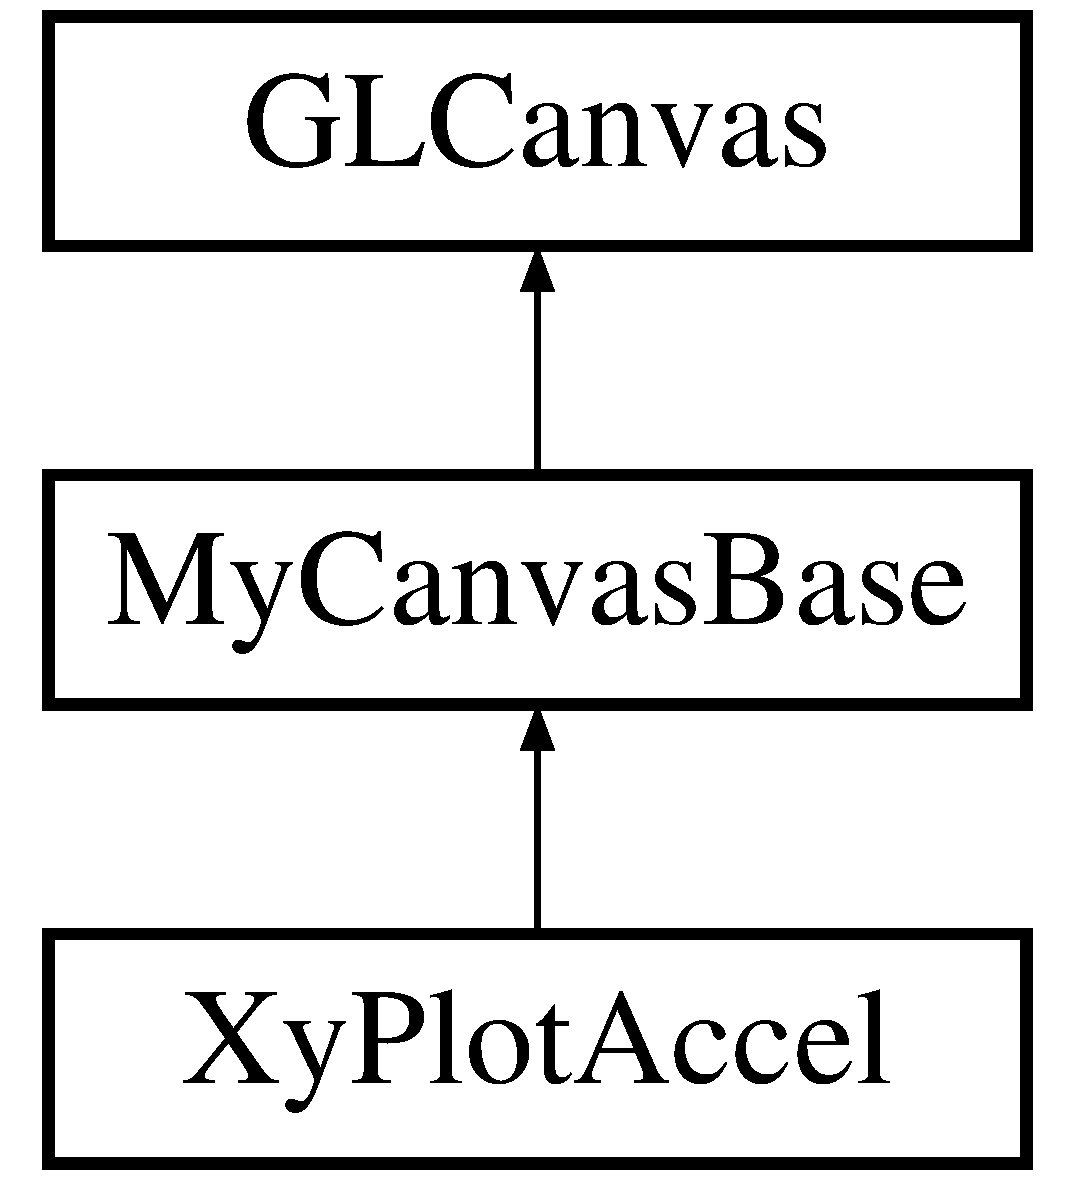
\includegraphics[height=3.000000cm]{classarbitros_ahrs_1_1_xy_plot_accel}
\end{center}
\end{figure}
\subsection*{Public Member Functions}
\begin{DoxyCompactItemize}
\item 
\hypertarget{classarbitros_ahrs_1_1_xy_plot_accel_aa5d4da6894799e330c531fcff2320723}{def {\bfseries Init\-G\-L}}\label{classarbitros_ahrs_1_1_xy_plot_accel_aa5d4da6894799e330c531fcff2320723}

\item 
\hypertarget{classarbitros_ahrs_1_1_xy_plot_accel_a06264628fa709c57ac53fe3f63080317}{def {\bfseries On\-Draw}}\label{classarbitros_ahrs_1_1_xy_plot_accel_a06264628fa709c57ac53fe3f63080317}

\end{DoxyCompactItemize}
\subsection*{Data Fields}
\begin{DoxyCompactItemize}
\item 
\hypertarget{classarbitros_ahrs_1_1_xy_plot_accel_aa3d6656320f1a7278c0c2c7fdf07617c}{{\bfseries size}}\label{classarbitros_ahrs_1_1_xy_plot_accel_aa3d6656320f1a7278c0c2c7fdf07617c}

\end{DoxyCompactItemize}


The documentation for this class was generated from the following file\-:\begin{DoxyCompactItemize}
\item 
C\-:/arbitros/trunk/boards/primus/examples/ins/python/arbitros\-Ahrs.\-py\end{DoxyCompactItemize}

\hypertarget{classarbitros_ahrs_1_1_xy_plot_gyro}{\section{Xy\-Plot\-Gyro Class Reference}
\label{classarbitros_ahrs_1_1_xy_plot_gyro}\index{Xy\-Plot\-Gyro@{Xy\-Plot\-Gyro}}
}
Inheritance diagram for Xy\-Plot\-Gyro\-:\begin{figure}[H]
\begin{center}
\leavevmode
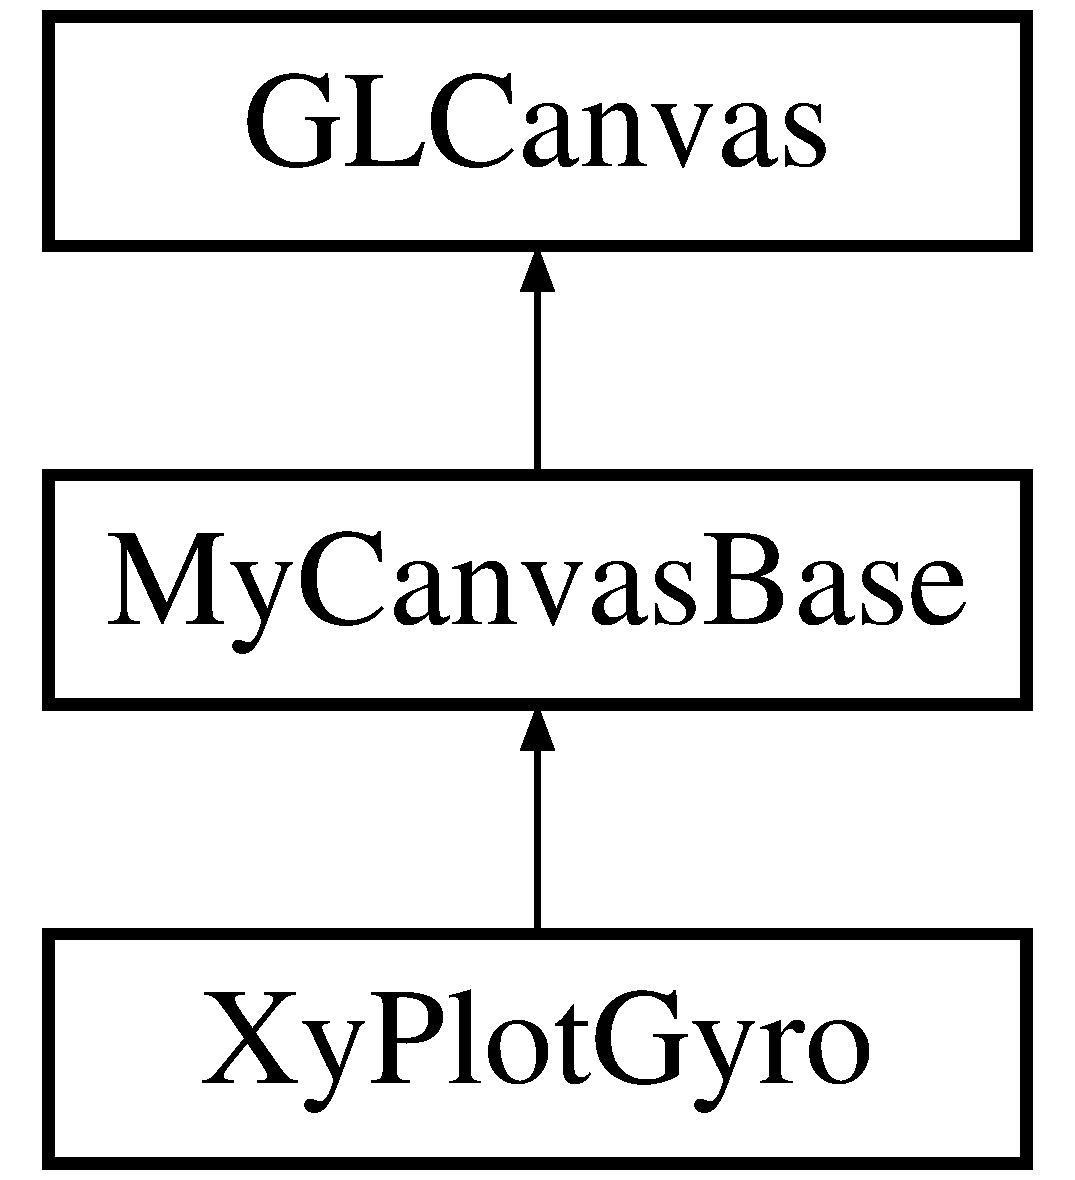
\includegraphics[height=3.000000cm]{classarbitros_ahrs_1_1_xy_plot_gyro}
\end{center}
\end{figure}
\subsection*{Public Member Functions}
\begin{DoxyCompactItemize}
\item 
\hypertarget{classarbitros_ahrs_1_1_xy_plot_gyro_aa5d4da6894799e330c531fcff2320723}{def {\bfseries Init\-G\-L}}\label{classarbitros_ahrs_1_1_xy_plot_gyro_aa5d4da6894799e330c531fcff2320723}

\item 
\hypertarget{classarbitros_ahrs_1_1_xy_plot_gyro_a06264628fa709c57ac53fe3f63080317}{def {\bfseries On\-Draw}}\label{classarbitros_ahrs_1_1_xy_plot_gyro_a06264628fa709c57ac53fe3f63080317}

\end{DoxyCompactItemize}
\subsection*{Data Fields}
\begin{DoxyCompactItemize}
\item 
\hypertarget{classarbitros_ahrs_1_1_xy_plot_gyro_aa3d6656320f1a7278c0c2c7fdf07617c}{{\bfseries size}}\label{classarbitros_ahrs_1_1_xy_plot_gyro_aa3d6656320f1a7278c0c2c7fdf07617c}

\end{DoxyCompactItemize}


The documentation for this class was generated from the following file\-:\begin{DoxyCompactItemize}
\item 
C\-:/arbitros/trunk/boards/primus/examples/ins/python/arbitros\-Ahrs.\-py\end{DoxyCompactItemize}

\hypertarget{classarbitros_ahrs_1_1_xy_plot_mag}{\section{Xy\-Plot\-Mag Class Reference}
\label{classarbitros_ahrs_1_1_xy_plot_mag}\index{Xy\-Plot\-Mag@{Xy\-Plot\-Mag}}
}
Inheritance diagram for Xy\-Plot\-Mag\-:\begin{figure}[H]
\begin{center}
\leavevmode
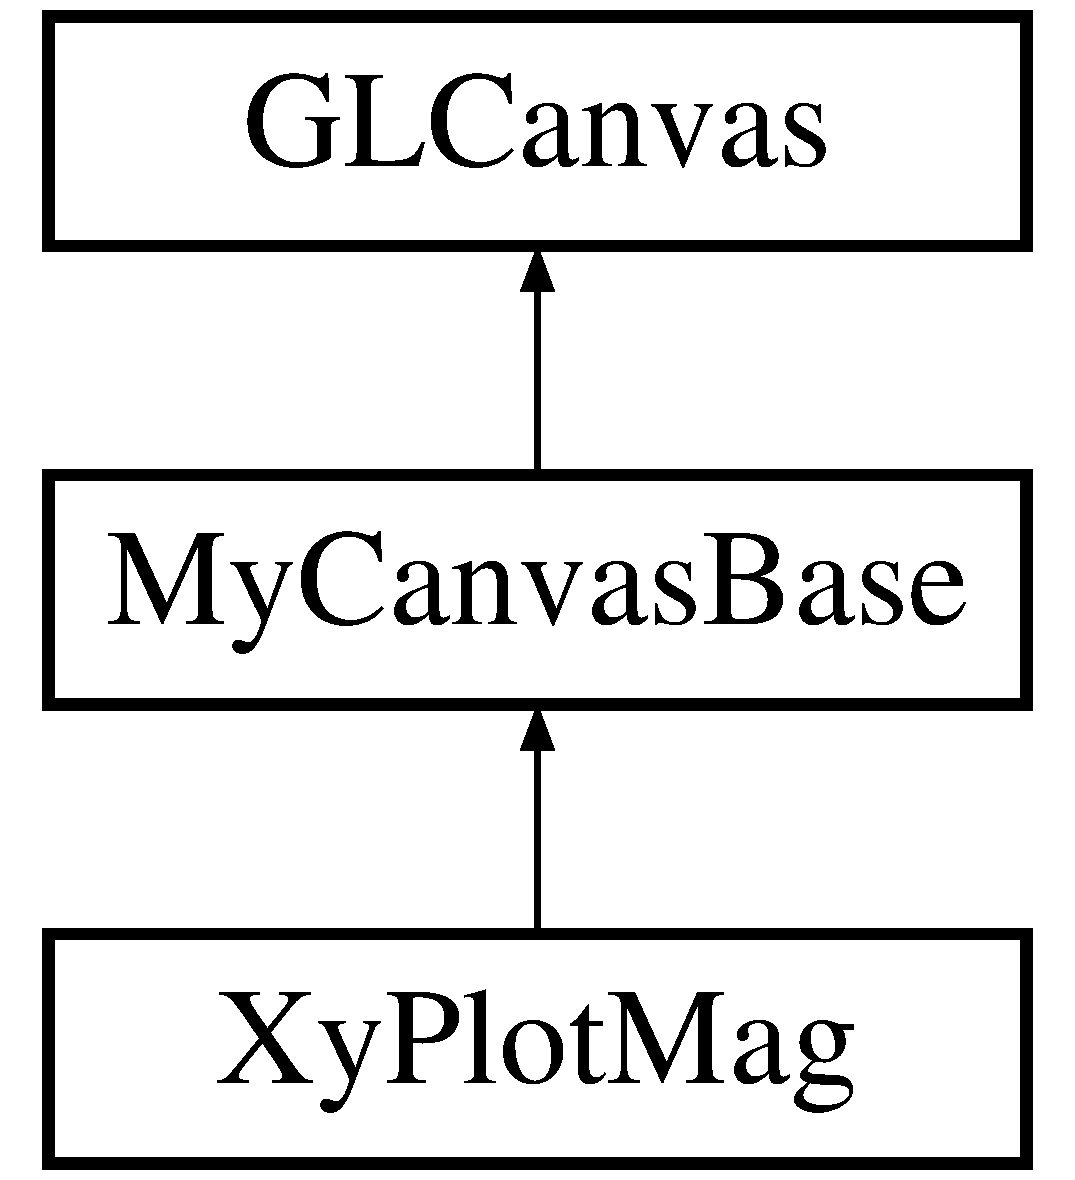
\includegraphics[height=3.000000cm]{classarbitros_ahrs_1_1_xy_plot_mag}
\end{center}
\end{figure}
\subsection*{Public Member Functions}
\begin{DoxyCompactItemize}
\item 
\hypertarget{classarbitros_ahrs_1_1_xy_plot_mag_aa5d4da6894799e330c531fcff2320723}{def {\bfseries Init\-G\-L}}\label{classarbitros_ahrs_1_1_xy_plot_mag_aa5d4da6894799e330c531fcff2320723}

\item 
\hypertarget{classarbitros_ahrs_1_1_xy_plot_mag_a06264628fa709c57ac53fe3f63080317}{def {\bfseries On\-Draw}}\label{classarbitros_ahrs_1_1_xy_plot_mag_a06264628fa709c57ac53fe3f63080317}

\end{DoxyCompactItemize}
\subsection*{Data Fields}
\begin{DoxyCompactItemize}
\item 
\hypertarget{classarbitros_ahrs_1_1_xy_plot_mag_aa3d6656320f1a7278c0c2c7fdf07617c}{{\bfseries size}}\label{classarbitros_ahrs_1_1_xy_plot_mag_aa3d6656320f1a7278c0c2c7fdf07617c}

\end{DoxyCompactItemize}


The documentation for this class was generated from the following file\-:\begin{DoxyCompactItemize}
\item 
C\-:/arbitros/trunk/boards/primus/examples/ins/python/arbitros\-Ahrs.\-py\end{DoxyCompactItemize}

\chapter{File Documentation}
\hypertarget{arb__console_8c}{\section{C\-:/arbitros/trunk/rtos/source/common/arb\-\_\-console.c File Reference}
\label{arb__console_8c}\index{C\-:/arbitros/trunk/rtos/source/common/arb\-\_\-console.\-c@{C\-:/arbitros/trunk/rtos/source/common/arb\-\_\-console.\-c}}
}


Main handler for the system console interface.  


{\ttfamily \#include $<$stdio.\-h$>$}\\*
{\ttfamily \#include $<$stdlib.\-h$>$}\\*
{\ttfamily \#include $<$string.\-h$>$}\\*
{\ttfamily \#include \char`\"{}arb\-\_\-error.\-h\char`\"{}}\\*
{\ttfamily \#include \char`\"{}arb\-\_\-thread.\-h\char`\"{}}\\*
{\ttfamily \#include \char`\"{}arb\-\_\-device.\-h\char`\"{}}\\*
{\ttfamily \#include \char`\"{}arb\-\_\-sys\-Timer.\-h\char`\"{}}\\*
{\ttfamily \#include \char`\"{}arb\-\_\-console.\-h\char`\"{}}\\*
{\ttfamily \#include \char`\"{}arb\-\_\-printf.\-h\char`\"{}}\\*
{\ttfamily \#include \char`\"{}arb\-\_\-scheduler.\-h\char`\"{}}\\*
{\ttfamily \#include \char`\"{}drv\-\_\-console.\-h\char`\"{}}\\*
{\ttfamily \#include \char`\"{}drv\-\_\-sd.\-h\char`\"{}}\\*
\subsection*{Data Structures}
\begin{DoxyCompactItemize}
\item 
struct \hyperlink{structt__console_object}{t\-\_\-console\-Object}
\begin{DoxyCompactList}\small\item\em Grouping of objects commonly used across all functions within this file. \end{DoxyCompactList}\end{DoxyCompactItemize}
\subsection*{Macros}
\begin{DoxyCompactItemize}
\item 
\hypertarget{arb__console_8c_adc53244b6829c70060f007f46bedf047}{\#define \hyperlink{arb__console_8c_adc53244b6829c70060f007f46bedf047}{P\-R\-I\-N\-T\-F\-\_\-\-N\-U\-M\-\_\-\-L\-I\-N\-E\-S\-\_\-\-T\-O\-\_\-\-P\-R\-I\-N\-T}~(20)}\label{arb__console_8c_adc53244b6829c70060f007f46bedf047}

\begin{DoxyCompactList}\small\item\em This macro controls the number of lines displayed to the terminal when printing the contents of a file using the command 'head'. \end{DoxyCompactList}\end{DoxyCompactItemize}
\subsection*{Functions}
\begin{DoxyCompactItemize}
\item 
static void \hyperlink{arb__console_8c_a53daff761c655e05e651b375d95d6309}{arb\-\_\-console} (t\-\_\-parameters t\-\_\-param, t\-\_\-arguments t\-\_\-args)
\begin{DoxyCompactList}\small\item\em Arbitros system console thread which controls reading and writing to the standard output (command window). \end{DoxyCompactList}\item 
static bool \hyperlink{arb__console_8c_a7ab5296ac37a44178c85af393cca3d44}{arb\-\_\-head} (int8\-\_\-t $\ast$pc\-\_\-buff, \hyperlink{structt__console_tok_hndl}{t\-\_\-console\-Tok\-Hndl} $\ast$pt\-\_\-tok\-Hndl)
\begin{DoxyCompactList}\small\item\em Reads the contents of a file and writes them to the command window. \end{DoxyCompactList}\item 
static void \hyperlink{arb__console_8c_a794d3adb2199bc2fea45b5c155e1a689}{arb\-\_\-display\-Kernel\-Help} (int8\-\_\-t $\ast$pc\-\_\-buff)
\begin{DoxyCompactList}\small\item\em Displays a list of kernel commands to the terminal window. \end{DoxyCompactList}\item 
static void \hyperlink{arb__console_8c_a7e29a86133dfa7660c4fd34c1535f51f}{arb\-\_\-set\-Debug\-Level} (\hyperlink{structt__console_tok_hndl}{t\-\_\-console\-Tok\-Hndl} $\ast$pt\-\_\-tok\-Hndl, int8\-\_\-t $\ast$pc\-\_\-buff)
\begin{DoxyCompactList}\small\item\em Puts the system into debug mode where \#arb\-\_\-printf information is written to the terminal. \end{DoxyCompactList}\item 
static void \hyperlink{arb__console_8c_a0ea3dea385ce66287f4eba9c06f4a8cb}{arb\-\_\-display\-Device\-List} (int8\-\_\-t $\ast$pc\-\_\-buff)
\item 
\hypertarget{arb__console_8c_a83957545ac8bc50184c4ce9dc4185971}{static void {\bfseries arb\-\_\-display\-System\-Statistics} (int8\-\_\-t $\ast$pc\-\_\-buff)}\label{arb__console_8c_a83957545ac8bc50184c4ce9dc4185971}

\item 
\hypertarget{arb__console_8c_a0750f79fe237bc0c9774b12f492d223e}{t\-\_\-error {\bfseries arb\-\_\-console\-Init} (char $\ast$pc\-\_\-cons\-Driver, char $\ast$pc\-\_\-sd\-Driver, t\-\_\-stack\-Size t\-\_\-stack, t\-\_\-thrd\-Prio t\-\_\-pri, bool($\ast$pf\-\_\-fun\-Ptr)(t\-\_\-\-D\-E\-V\-H\-A\-N\-D\-L\-E t\-\_\-console\-Hndl, int8\-\_\-t $\ast$pc\-\_\-buff, \hyperlink{structt__console_tok_hndl}{t\-\_\-console\-Tok\-Hndl} $\ast$pt\-\_\-tok\-Hndl))}\label{arb__console_8c_a0750f79fe237bc0c9774b12f492d223e}

\end{DoxyCompactItemize}
\subsection*{Variables}
\begin{DoxyCompactItemize}
\item 
\hypertarget{arb__console_8c_a7372a07169bf9ab879a82fb473517994}{static \hyperlink{structt__console_object}{t\-\_\-console\-Object} \hyperlink{arb__console_8c_a7372a07169bf9ab879a82fb473517994}{gt\-\_\-con\-Object}}\label{arb__console_8c_a7372a07169bf9ab879a82fb473517994}

\begin{DoxyCompactList}\small\item\em Global variable containing objects common to all the functions within the file \hyperlink{arb__console_8c}{arb\-\_\-console.\-c}. \end{DoxyCompactList}\end{DoxyCompactItemize}


\subsection{Detailed Description}
Main handler for the system console interface. This file defines a set of functions that provide the tools for interfacing with the operating system or user-\/space application via a terminal window. The primary handler is a blocking thread named \hyperlink{arb__console_8c_a53daff761c655e05e651b375d95d6309}{arb\-\_\-console}, which wakes any time a message is is received over the terminal via the device driver drv\-\_\-console.\-c. The following figure demonstrates how messages are exchanged and validated between the driver, console thread, and user-\/space handler.  After waking, the thread validates the tokenized message by checking the first entry against a list of basic kernel commands ({\bfseries ls, cd, help, dev, top, sdl, rm, sct, and head}). If the token doesn't match, the entire message is routed to the user-\/space layer for further evaluation. After processing the message the user-\/space layer returns control back to \hyperlink{arb__console_8c_a53daff761c655e05e651b375d95d6309}{arb\-\_\-console} with an indicator letting the thread know if the message was handled properly.

Standard Output (Terminal)  As seen in the figure, Arbitros offers a rich set of terminal commands. The first command {\bfseries ls}, outputs a list of all the directories and files currently housed on the system. In this example, only the 'L\-O\-G\-S' directory with 'D\-M\-S\-G.\-T\-X\-T' is present. These particular files are created during system initialization and used by the function \#arb\-\_\-printf for logging user-\/space or kernel debug messages. The {\bfseries help} command lists all the commands--with descriptions--recognized by the terminal handler \hyperlink{arb__console_8c_a53daff761c655e05e651b375d95d6309}{arb\-\_\-console}. Finally, the command {\bfseries dev} displays a list of all the device drivers and number of open device driver handles.  The second figure highlights the commands {\bfseries top, sdl, and rm}. The command {\bfseries top} displays metrics such as the size of various memory sections (.data, .bss, and .heap), as well as the amount R\-A\-M left on the system. Additionally, {\bfseries top} displays an estimate of processor thread loading comprised of metrics averaged over a one minute and five minute interval. This feature allows an Arbitros developer to tune the performance of a particular thread or collection of threads in order to minimize the burden on the system. The command {\bfseries sdl} with argument 0,1, or 2 turns on one of \#arb\-\_\-printf's three debug levels \#\-P\-R\-I\-N\-T\-F\-\_\-\-D\-B\-G\-\_\-\-L\-O\-W, \#\-P\-R\-I\-N\-T\-F\-\_\-\-D\-B\-G\-\_\-\-M\-E\-D, and \#\-P\-R\-I\-N\-T\-F\-\_\-\-D\-B\-G\-\_\-\-H\-I\-G\-H, respectively. As seen in the figure, {\bfseries sdl 0} enables the lowest debug level \#\-P\-R\-I\-N\-T\-F\-\_\-\-D\-B\-G\-\_\-\-L\-O\-W, which displays a message every time the thread \#arb\-\_\-idle resets the system watchdog timer. This particular debug configuration will tell the kernel to pass any priority \#arb\-\_\-printf debug message onto the terminal. Increasing the debug level, such as configuring {\bfseries sdl 1 (or 2)}, will tell Arbitros to pass \#arb\-\_\-printf messages with the same or higher priority onto the terminal. The ability to display messages based on priority eases software integration, allowing a developer to \char`\"{}de-\/clutter\char`\"{} the terminal output in order to highlight the most important information. The final command {\bfseries rm -\/r}, recursively removes all files and folders stored on the system flash drive.

\begin{DoxyCopyright}{Copyright}
Copyright (C) 2011-\/2013 Ryan M. Murphy $<$ryan.\-m.\-murphy.\-77. com$>$ This program is free software\-: you can redistribute it and/ or modify it under the terms of the G\-N\-U General Public License as published by the Free Software Foundation, either version 3 of the License, or (at your option) any later version. This program is distributed in the hope that it will be useful, but W\-I\-T\-H\-O\-U\-T A\-N\-Y W\-A\-R\-R\-A\-N\-T\-Y; without even the implied warranty of M\-E\-R\-C\-H\-A\-N\-T\-A\-B\-I\-L\-I\-T\-Y or F\-I\-T\-N\-E\-S\-S F\-O\-R A P\-A\-R\-T\-I\-C\-U\-L\-A\-R P\-U\-R\-P\-O\-S\-E. See the G\-N\-U General Public License for more details. You should have received a copy of the G\-N\-U General Public License along with this program. If not, see \href{http://www.gnu.org/licenses/}{\tt http\-://www.\-gnu.\-org/licenses/}.
\end{DoxyCopyright}
\begin{DoxyAuthor}{Author}
Ryan M. Murphy \href{mailto:ryan.m.murphy.77@gmail.com}{\tt ryan.\-m.\-murphy.\-77@gmail.\-com}
\end{DoxyAuthor}
\begin{DoxyDate}{Date}
Jan, 14, 2013
\end{DoxyDate}
\begin{DoxyVersion}{Version}
1.\-0 
\end{DoxyVersion}


\subsection{Function Documentation}
\hypertarget{arb__console_8c_a53daff761c655e05e651b375d95d6309}{\index{arb\-\_\-console.\-c@{arb\-\_\-console.\-c}!arb\-\_\-console@{arb\-\_\-console}}
\index{arb\-\_\-console@{arb\-\_\-console}!arb_console.c@{arb\-\_\-console.\-c}}
\subsubsection[{arb\-\_\-console}]{\setlength{\rightskip}{0pt plus 5cm}static void arb\-\_\-console (
\begin{DoxyParamCaption}
\item[{t\-\_\-parameters}]{t\-\_\-param, }
\item[{t\-\_\-arguments}]{t\-\_\-args}
\end{DoxyParamCaption}
)\hspace{0.3cm}{\ttfamily [static]}}}\label{arb__console_8c_a53daff761c655e05e651b375d95d6309}


Arbitros system console thread which controls reading and writing to the standard output (command window). 

This console thread provides a mechanism for exchanging text messages between an external user--via a command line interface --and Arbitros kernel or user-\/space application. The thread blocks until detecting a carriage return, from which it wakes and reads the contents of the device driver's (drv\-\_\-console.\-c) buffer. The new message is checked against a set of 'Linux like' Arbitros kernel commands such as; {\bfseries sct, help, sdl, dev, top, ls, rm, cd, and head}. If the message is recognized as a kernel command it is subsequently processed; otherwise, control of the console is passed onto the user-\/space application via a function pointer passed in as a parameter to \#arb\-\_\-console\-Init during system initialization.


\begin{DoxyParams}[1]{Parameters}
\mbox{\tt in}  & {\em t\-\_\-param} & User-\/definable parameter passed in at time of thread initialization.\\
\hline
\mbox{\tt in}  & {\em t\-\_\-args} & User-\/definable argument passed in at time of thread initialization.\\
\hline
\end{DoxyParams}
\begin{DoxyReturn}{Returns}
None. 
\end{DoxyReturn}
\hypertarget{arb__console_8c_a0ea3dea385ce66287f4eba9c06f4a8cb}{\index{arb\-\_\-console.\-c@{arb\-\_\-console.\-c}!arb\-\_\-display\-Device\-List@{arb\-\_\-display\-Device\-List}}
\index{arb\-\_\-display\-Device\-List@{arb\-\_\-display\-Device\-List}!arb_console.c@{arb\-\_\-console.\-c}}
\subsubsection[{arb\-\_\-display\-Device\-List}]{\setlength{\rightskip}{0pt plus 5cm}static void arb\-\_\-display\-Device\-List (
\begin{DoxyParamCaption}
\item[{int8\-\_\-t $\ast$}]{pc\-\_\-buff}
\end{DoxyParamCaption}
)\hspace{0.3cm}{\ttfamily [static]}}}\label{arb__console_8c_a0ea3dea385ce66287f4eba9c06f4a8cb}

\begin{DoxyParams}[1]{Parameters}
\mbox{\tt in}  & {\em pc\-\_\-buff} & Scratch buffer used for writing messages to the terminal.\\
\hline
\end{DoxyParams}
\begin{DoxyReturn}{Returns}
None. 
\end{DoxyReturn}
\hypertarget{arb__console_8c_a794d3adb2199bc2fea45b5c155e1a689}{\index{arb\-\_\-console.\-c@{arb\-\_\-console.\-c}!arb\-\_\-display\-Kernel\-Help@{arb\-\_\-display\-Kernel\-Help}}
\index{arb\-\_\-display\-Kernel\-Help@{arb\-\_\-display\-Kernel\-Help}!arb_console.c@{arb\-\_\-console.\-c}}
\subsubsection[{arb\-\_\-display\-Kernel\-Help}]{\setlength{\rightskip}{0pt plus 5cm}static void arb\-\_\-display\-Kernel\-Help (
\begin{DoxyParamCaption}
\item[{int8\-\_\-t $\ast$}]{pc\-\_\-buff}
\end{DoxyParamCaption}
)\hspace{0.3cm}{\ttfamily [static]}}}\label{arb__console_8c_a794d3adb2199bc2fea45b5c155e1a689}


Displays a list of kernel commands to the terminal window. 

After the thread \hyperlink{arb__console_8c_a53daff761c655e05e651b375d95d6309}{arb\-\_\-console} receives the {\bfseries help} command via the terminal window it calls this function in order to display a list of all possible kernel commands.


\begin{DoxyParams}[1]{Parameters}
\mbox{\tt in}  & {\em pc\-\_\-buff} & scratch buffer used for writing the kernel commands and their description to the terminal window.\\
\hline
\end{DoxyParams}
\begin{DoxyReturn}{Returns}
None. 
\end{DoxyReturn}
\hypertarget{arb__console_8c_a7ab5296ac37a44178c85af393cca3d44}{\index{arb\-\_\-console.\-c@{arb\-\_\-console.\-c}!arb\-\_\-head@{arb\-\_\-head}}
\index{arb\-\_\-head@{arb\-\_\-head}!arb_console.c@{arb\-\_\-console.\-c}}
\subsubsection[{arb\-\_\-head}]{\setlength{\rightskip}{0pt plus 5cm}static bool arb\-\_\-head (
\begin{DoxyParamCaption}
\item[{int8\-\_\-t $\ast$}]{pc\-\_\-buff, }
\item[{{\bf t\-\_\-console\-Tok\-Hndl} $\ast$}]{pt\-\_\-tok\-Hndl}
\end{DoxyParamCaption}
)\hspace{0.3cm}{\ttfamily [static]}}}\label{arb__console_8c_a7ab5296ac37a44178c85af393cca3d44}


Reads the contents of a file and writes them to the command window. 

This function prints the contents of the file (pointed to by {\bfseries  pt\-\_\-tok\-Hndl}) entered via the terminal window using the command {\bfseries head $<$filename$>$}. The file is iteratively printed \hyperlink{arb__console_8c_adc53244b6829c70060f007f46bedf047}{P\-R\-I\-N\-T\-F\-\_\-\-N\-U\-M\-\_\-\-L\-I\-N\-E\-S\-\_\-\-T\-O\-\_\-\-P\-R\-I\-N\-T} lines at a time. At the end of each iteration, the user is asked if another \hyperlink{arb__console_8c_adc53244b6829c70060f007f46bedf047}{P\-R\-I\-N\-T\-F\-\_\-\-N\-U\-M\-\_\-\-L\-I\-N\-E\-S\-\_\-\-T\-O\-\_\-\-P\-R\-I\-N\-T} lines should be displayed or if termination is required.


\begin{DoxyParams}[1]{Parameters}
\mbox{\tt in}  & {\em pc\-\_\-buff} & Scratch buffer used for reading/writing messages between the command window and system console thread \hyperlink{arb__console_8c_a53daff761c655e05e651b375d95d6309}{arb\-\_\-console}.\\
\hline
\mbox{\tt in}  & {\em pt\-\_\-tok\-Hndl} & pointer to the current list of command line tokens.\\
\hline
\end{DoxyParams}
\begin{DoxyReturn}{Returns}
'true', if the file ($<$filename$>$) was opened, otherwise 'false'. 
\end{DoxyReturn}
\hypertarget{arb__console_8c_a7e29a86133dfa7660c4fd34c1535f51f}{\index{arb\-\_\-console.\-c@{arb\-\_\-console.\-c}!arb\-\_\-set\-Debug\-Level@{arb\-\_\-set\-Debug\-Level}}
\index{arb\-\_\-set\-Debug\-Level@{arb\-\_\-set\-Debug\-Level}!arb_console.c@{arb\-\_\-console.\-c}}
\subsubsection[{arb\-\_\-set\-Debug\-Level}]{\setlength{\rightskip}{0pt plus 5cm}static void arb\-\_\-set\-Debug\-Level (
\begin{DoxyParamCaption}
\item[{{\bf t\-\_\-console\-Tok\-Hndl} $\ast$}]{pt\-\_\-tok\-Hndl, }
\item[{int8\-\_\-t $\ast$}]{pc\-\_\-buff}
\end{DoxyParamCaption}
)\hspace{0.3cm}{\ttfamily [static]}}}\label{arb__console_8c_a7e29a86133dfa7660c4fd34c1535f51f}


Puts the system into debug mode where \#arb\-\_\-printf information is written to the terminal. 

After the thread \hyperlink{arb__console_8c_a53daff761c655e05e651b375d95d6309}{arb\-\_\-console()} receives a {\bfseries sdl $<$arg$>$} command, it calls this function in order to configure the system--both kernel and console interface--for writing debug information to terminal window. If there are software debug messages (i.\-e. \#arb\-\_\-printf) with priority equal to or higher than $<$arg$>$ (e.\-g. 0,1, 2) they will subsequently be displayed at the terminal output; otherwise, the terminal will remain blank. After entering this mode, the user can press the return key--at any time--in order to return to nominal console operation. \begin{DoxySeeAlso}{See Also}
term for further information
\end{DoxySeeAlso}

\begin{DoxyParams}[1]{Parameters}
\mbox{\tt in}  & {\em pc\-\_\-buff} & Scratch buffer used for writing messages to the terminal.\\
\hline
\mbox{\tt in}  & {\em pt\-\_\-tok\-Hndl} & pointer to the tokenized list of terminal commands and arguments.\\
\hline
\end{DoxyParams}
\begin{DoxyReturn}{Returns}
None. 
\end{DoxyReturn}

\hypertarget{arb__main_8c}{\section{C\-:/arbitros/trunk/rtos/source/common/arb\-\_\-main.c File Reference}
\label{arb__main_8c}\index{C\-:/arbitros/trunk/rtos/source/common/arb\-\_\-main.\-c@{C\-:/arbitros/trunk/rtos/source/common/arb\-\_\-main.\-c}}
}


Main code entry point.  


{\ttfamily \#include \char`\"{}arb\-\_\-scheduler.\-h\char`\"{}}\\*
{\ttfamily \#include \char`\"{}arb\-\_\-printf.\-h\char`\"{}}\\*
{\ttfamily \#include \char`\"{}utl\-\_\-clocks.\-h\char`\"{}}\\*
{\ttfamily \#include \char`\"{}utl\-\_\-pmic.\-h\char`\"{}}\\*
\subsection*{Functions}
\begin{DoxyCompactItemize}
\item 
\hypertarget{arb__main_8c_a047774f8c6a581a4a86322aaba2f2e15}{void {\bfseries usr\-\_\-app\-Init} (void)}\label{arb__main_8c_a047774f8c6a581a4a86322aaba2f2e15}

\item 
int \hyperlink{arb__main_8c_a840291bc02cba5474a4cb46a9b9566fe}{main} (void)
\begin{DoxyCompactList}\small\item\em Performs power-\/on system initialization. \end{DoxyCompactList}\end{DoxyCompactItemize}


\subsection{Detailed Description}
Main code entry point. This file calls four main tasks after system power-\/on for the purpose of platform initialization. The first task \#utl\-\_\-set\-Cpu\-Freq, configures the default C\-P\-U frequency. The second function \#utl\-\_\-configure\-Int\-Level, sets the nominal interrupt level--nested interrupts are not allowed. The third function \#usr\-\_\-app\-Init, hands over control to the user-\/space layer for the purpose of device driver registration, scheduler initialization, and user-\/space thread configuration. Implementation of this function is required of all user-\/space applications; however, the particular operations performed within are application dependent. Meaning, the choice of a particular device driver to include or a particular kernel setting (like logging \#arb\-\_\-printf data to an S\-D card) is completely up to the user-\/space application developer. After completion of the call to \#usr\-\_\-app\-Init, control is passed back to \hyperlink{arb__main_8c_a840291bc02cba5474a4cb46a9b9566fe}{main} where the first thread gets launched after completing the call to \#arb\-\_\-scheduler\-Start.

\begin{DoxyCopyright}{Copyright}
Copyright (C) 2011-\/2013 Ryan M. Murphy $<$ryan.\-m.\-murphy.\-77. com$>$ This program is free software\-: you can redistribute it and/ or modify it under the terms of the G\-N\-U General Public License as published by the Free Software Foundation, either version 3 of the License, or (at your option) any later version. This program is distributed in the hope that it will be useful, but W\-I\-T\-H\-O\-U\-T A\-N\-Y W\-A\-R\-R\-A\-N\-T\-Y; without even the implied warranty of M\-E\-R\-C\-H\-A\-N\-T\-A\-B\-I\-L\-I\-T\-Y or F\-I\-T\-N\-E\-S\-S F\-O\-R A P\-A\-R\-T\-I\-C\-U\-L\-A\-R P\-U\-R\-P\-O\-S\-E. See the G\-N\-U General Public License for more details. You should have received a copy of the G\-N\-U General Public License along with this program. If not, see \href{http://www.gnu.org/licenses/}{\tt http\-://www.\-gnu.\-org/licenses/}.
\end{DoxyCopyright}
\begin{DoxyAuthor}{Author}
Ryan M. Murphy \href{mailto:ryan.m.murphy.77@gmail.com}{\tt ryan.\-m.\-murphy.\-77@gmail.\-com}
\end{DoxyAuthor}
\begin{DoxyDate}{Date}
September 26, 2012
\end{DoxyDate}
\begin{DoxyVersion}{Version}
1.\-0 
\end{DoxyVersion}


\subsection{Function Documentation}
\hypertarget{arb__main_8c_a840291bc02cba5474a4cb46a9b9566fe}{\index{arb\-\_\-main.\-c@{arb\-\_\-main.\-c}!main@{main}}
\index{main@{main}!arb_main.c@{arb\-\_\-main.\-c}}
\subsubsection[{main}]{\setlength{\rightskip}{0pt plus 5cm}int main (
\begin{DoxyParamCaption}
\item[{void}]{}
\end{DoxyParamCaption}
)}}\label{arb__main_8c_a840291bc02cba5474a4cb46a9b9566fe}


Performs power-\/on system initialization. 

\begin{DoxyReturn}{Returns}
Function never returns. 
\end{DoxyReturn}

\hypertarget{avr__compiler_8h}{\section{C\-:/arbitros/trunk/utilities/headers/xmega128\-A1/avr\-\_\-compiler.h File Reference}
\label{avr__compiler_8h}\index{C\-:/arbitros/trunk/utilities/headers/xmega128\-A1/avr\-\_\-compiler.\-h@{C\-:/arbitros/trunk/utilities/headers/xmega128\-A1/avr\-\_\-compiler.\-h}}
}


This file implements some macros that makes the I\-A\-R C-\/compiler and avr-\/gcc work with the same code base for the A\-V\-R architecture.  


{\ttfamily \#include $<$stdint.\-h$>$}\\*
{\ttfamily \#include $<$stdbool.\-h$>$}\\*
{\ttfamily \#include $<$stdlib.\-h$>$}\\*
\subsection*{Macros}
\begin{DoxyCompactItemize}
\item 
\hypertarget{avr__compiler_8h_a43bafb28b29491ec7f871319b5a3b2f8}{\#define \hyperlink{avr__compiler_8h_a43bafb28b29491ec7f871319b5a3b2f8}{F\-\_\-\-C\-P\-U}~32000000\-U\-L}\label{avr__compiler_8h_a43bafb28b29491ec7f871319b5a3b2f8}

\begin{DoxyCompactList}\small\item\em Define default C\-P\-U frequency, if this is not already defined. \end{DoxyCompactList}\item 
\#define \hyperlink{avr__compiler_8h_a0a4fb62f9e69209c9c8c8e34ebb3df6f}{A\-V\-R\-\_\-\-E\-N\-T\-E\-R\-\_\-\-C\-R\-I\-T\-I\-C\-A\-L\-\_\-\-R\-E\-G\-I\-O\-N}()
\begin{DoxyCompactList}\small\item\em This macro will protect the following code from interrupts. \end{DoxyCompactList}\item 
\hypertarget{avr__compiler_8h_a770b47b04eec57748be0826a3d23503b}{\#define \hyperlink{avr__compiler_8h_a770b47b04eec57748be0826a3d23503b}{A\-V\-R\-\_\-\-L\-E\-A\-V\-E\-\_\-\-C\-R\-I\-T\-I\-C\-A\-L\-\_\-\-R\-E\-G\-I\-O\-N}()~S\-R\-E\-G = saved\-\_\-sreg;}\label{avr__compiler_8h_a770b47b04eec57748be0826a3d23503b}

\begin{DoxyCompactList}\small\item\em This macro must always be used in conjunction with A\-V\-R\-\_\-\-E\-N\-T\-E\-R\-\_\-\-C\-R\-I\-T\-I\-C\-A\-L\-\_\-\-R\-E\-G\-I\-O\-N so the interrupts are enabled again. \end{DoxyCompactList}\end{DoxyCompactItemize}


\subsection{Detailed Description}
This file implements some macros that makes the I\-A\-R C-\/compiler and avr-\/gcc work with the same code base for the A\-V\-R architecture. \begin{DoxyParagraph}{Documentation}
For comprehensive code documentation, supported compilers, compiler settings and supported devices see readme.\-html
\end{DoxyParagraph}
\begin{DoxyAuthor}{Author}
Atmel Corporation\-: \href{http://www.atmel.com}{\tt http\-://www.\-atmel.\-com} \par
 Support email\-: \href{mailto:avr@atmel.com}{\tt avr@atmel.\-com}
\end{DoxyAuthor}
\begin{DoxyParagraph}{Revision\-:}
2772 
\end{DoxyParagraph}
\begin{DoxyParagraph}{Date\-:}
2009-\/09-\/11 12\-:40\-:26 +0200 (fr, 11 sep 2009) 
\end{DoxyParagraph}
\par


Copyright (c) 2008, Atmel Corporation All rights reserved.

Redistribution and use in source and binary forms, with or without modification, are permitted provided that the following conditions are met\-:


\begin{DoxyEnumerate}
\item Redistributions of source code must retain the above copyright notice, this list of conditions and the following disclaimer.
\end{DoxyEnumerate}


\begin{DoxyEnumerate}
\item Redistributions in binary form must reproduce the above copyright notice, this list of conditions and the following disclaimer in the documentation and/or other materials provided with the distribution.
\end{DoxyEnumerate}


\begin{DoxyEnumerate}
\item The name of A\-T\-M\-E\-L may not be used to endorse or promote products derived from this software without specific prior written permission.
\end{DoxyEnumerate}

T\-H\-I\-S S\-O\-F\-T\-W\-A\-R\-E I\-S P\-R\-O\-V\-I\-D\-E\-D B\-Y A\-T\-M\-E\-L \char`\"{}\-A\-S I\-S\char`\"{} A\-N\-D A\-N\-Y E\-X\-P\-R\-E\-S\-S O\-R I\-M\-P\-L\-I\-E\-D W\-A\-R\-R\-A\-N\-T\-I\-E\-S, I\-N\-C\-L\-U\-D\-I\-N\-G, B\-U\-T N\-O\-T L\-I\-M\-I\-T\-E\-D T\-O, T\-H\-E I\-M\-P\-L\-I\-E\-D W\-A\-R\-R\-A\-N\-T\-I\-E\-S O\-F M\-E\-R\-C\-H\-A\-N\-T\-A\-B\-I\-L\-I\-T\-Y A\-N\-D F\-I\-T\-N\-E\-S\-S F\-O\-R A P\-A\-R\-T\-I\-C\-U\-L\-A\-R P\-U\-R\-P\-O\-S\-E A\-R\-E E\-X\-P\-R\-E\-S\-S\-L\-Y A\-N\-D S\-P\-E\-C\-I\-F\-I\-C\-A\-L\-L\-Y D\-I\-S\-C\-L\-A\-I\-M\-E\-D. I\-N N\-O E\-V\-E\-N\-T S\-H\-A\-L\-L A\-T\-M\-E\-L B\-E L\-I\-A\-B\-L\-E F\-O\-R A\-N\-Y D\-I\-R\-E\-C\-T, I\-N\-D\-I\-R\-E\-C\-T, I\-N\-C\-I\-D\-E\-N\-T\-A\-L, S\-P\-E\-C\-I\-A\-L, E\-X\-E\-M\-P\-L\-A\-R\-Y, O\-R C\-O\-N\-S\-E\-Q\-U\-E\-N\-T\-I\-A\-L D\-A\-M\-A\-G\-E\-S (I\-N\-C\-L\-U\-D\-I\-N\-G, B\-U\-T N\-O\-T L\-I\-M\-I\-T\-E\-D T\-O, P\-R\-O\-C\-U\-R\-E\-M\-E\-N\-T O\-F S\-U\-B\-S\-T\-I\-T\-U\-T\-E G\-O\-O\-D\-S O\-R S\-E\-R\-V\-I\-C\-E\-S; L\-O\-S\-S O\-F U\-S\-E, D\-A\-T\-A, O\-R P\-R\-O\-F\-I\-T\-S; O\-R B\-U\-S\-I\-N\-E\-S\-S I\-N\-T\-E\-R\-R\-U\-P\-T\-I\-O\-N) H\-O\-W\-E\-V\-E\-R C\-A\-U\-S\-E\-D A\-N\-D O\-N A\-N\-Y T\-H\-E\-O\-R\-Y O\-F L\-I\-A\-B\-I\-L\-I\-T\-Y, W\-H\-E\-T\-H\-E\-R I\-N C\-O\-N\-T\-R\-A\-C\-T, S\-T\-R\-I\-C\-T L\-I\-A\-B\-I\-L\-I\-T\-Y, O\-R T\-O\-R\-T (I\-N\-C\-L\-U\-D\-I\-N\-G N\-E\-G\-L\-I\-G\-E\-N\-C\-E O\-R O\-T\-H\-E\-R\-W\-I\-S\-E) A\-R\-I\-S\-I\-N\-G I\-N A\-N\-Y W\-A\-Y O\-U\-T O\-F T\-H\-E U\-S\-E O\-F T\-H\-I\-S S\-O\-F\-T\-W\-A\-R\-E, E\-V\-E\-N I\-F A\-D\-V\-I\-S\-E\-D O\-F T\-H\-E P\-O\-S\-S\-I\-B\-I\-L\-I\-T\-Y O\-F S\-U\-C\-H D\-A\-M\-A\-G\-E. 

\subsection{Macro Definition Documentation}
\hypertarget{avr__compiler_8h_a0a4fb62f9e69209c9c8c8e34ebb3df6f}{\index{avr\-\_\-compiler.\-h@{avr\-\_\-compiler.\-h}!A\-V\-R\-\_\-\-E\-N\-T\-E\-R\-\_\-\-C\-R\-I\-T\-I\-C\-A\-L\-\_\-\-R\-E\-G\-I\-O\-N@{A\-V\-R\-\_\-\-E\-N\-T\-E\-R\-\_\-\-C\-R\-I\-T\-I\-C\-A\-L\-\_\-\-R\-E\-G\-I\-O\-N}}
\index{A\-V\-R\-\_\-\-E\-N\-T\-E\-R\-\_\-\-C\-R\-I\-T\-I\-C\-A\-L\-\_\-\-R\-E\-G\-I\-O\-N@{A\-V\-R\-\_\-\-E\-N\-T\-E\-R\-\_\-\-C\-R\-I\-T\-I\-C\-A\-L\-\_\-\-R\-E\-G\-I\-O\-N}!avr_compiler.h@{avr\-\_\-compiler.\-h}}
\subsubsection[{A\-V\-R\-\_\-\-E\-N\-T\-E\-R\-\_\-\-C\-R\-I\-T\-I\-C\-A\-L\-\_\-\-R\-E\-G\-I\-O\-N}]{\setlength{\rightskip}{0pt plus 5cm}\#define A\-V\-R\-\_\-\-E\-N\-T\-E\-R\-\_\-\-C\-R\-I\-T\-I\-C\-A\-L\-\_\-\-R\-E\-G\-I\-O\-N(
\begin{DoxyParamCaption}
{}
\end{DoxyParamCaption}
)}}\label{avr__compiler_8h_a0a4fb62f9e69209c9c8c8e34ebb3df6f}
{\bfseries Value\-:}
\begin{DoxyCode}
uint8\_t \textcolor{keyword}{volatile} saved\_sreg = SREG; \(\backslash\)
                                     cli();
\end{DoxyCode}


This macro will protect the following code from interrupts. 


\addcontentsline{toc}{part}{Index}
\printindex
\end{document}
